%\documentclass[letterpaper,twocolumn,10pt]{article}
\documentclass{cls/hotnets16}

\setlength{\pdfpagewidth}{8.5in}
\setlength{\pdfpageheight}{11in}

\usepackage{amsmath,amssymb}
\usepackage{times}
\usepackage{xcolor}
\usepackage{graphics}
\usepackage{xspace}
\usepackage{amsmath, amssymb}
\usepackage[hyphenbreaks]{breakurl}
\usepackage[hyphens]{url}
\usepackage{hyperref}
\usepackage{subfigure}
\usepackage[font=bf,labelfont=bf]{caption}

\newcommand{\tabincell}[2]{\begin{tabular}{@{}#1@{}}#2\end{tabular}}
\newcommand{\summation}[2]{\ensuremath{\displaystyle\sum\limits_{#1}^{#2}}}
\newcommand{\rbr}[1]{\left(#1\right)}
\newcommand{\cbr}[1]{\left\{#1\right\}}

\renewcommand\textfloatsep{0.05in}
\renewcommand\abovecaptionskip{0.05in}
\renewcommand\belowcaptionskip{0.05in}
\renewcommand\dbltextfloatsep{0.05in}

\def\todo#1{{\textcolor{red}{TODO: {\sf #1}}}}
\def\harry#1{{\textcolor{purple}{harry: {\sf #1}}}}
\newcommand{\vyas}[1]{{\footnotesize\color{red}[VS: #1]}}

\def\para#1{\vspace{0.05in}\noindent\textbf{#1}\hspace{0.1in}}

\newcommand{\sysname}{{\small {\sf C-Verbs}}\xspace}
\newcommand{\myeqn}[1]{{\small $#1$ \normalsize}}

\begin{document}

\title{Emancipating Your Containers for Full Network Speed
 \\ \vyas{this is probably the most boring hotnets title you can pick :) .. i would pick 
 something to highlight this is a new problem and you have a new idea -- high perf/low ovehread sounds like a boring ATC paper not hotnets !}\harry{I cannot agree more :), but this is the hardest part. Give me some time.}}

\date{}


\maketitle
\thispagestyle{empty}

\textbf{Abstract---} 
With the tremendous popularity gained by container technology, many applications are being containerized:
splitting into numerous containers connected by networks. However, current container networking solutions
have either bad performance or poor portability, which undermines the advantages of containerization.
In this paper, we propose \sysname, a container networking solution which achieves both high performance
and good portability. \sysname is designed according to the observation that strict isolations are unnecessary 
among containers trusting each other, and it can significantly boost the communication quality of containers by 
compromising isolation a little bit. Specifically, we enable containers on the same physical machine
to communicate via shared-memory and the ones on different physical machines communicate via
high performance networking options, e.g. RDMA and DPDK. Naively wrapping up all the solutions
together will result in poor potability of containers and huge complexity in application development.
Instead, \sysname leverages a network abstraction which supports all common network APIs and 
a centralized network orchestrator which decides how to deliver data transparently to applications in the containers.
\section{Introduction} 
\label{sec:introduction}

\begin{quote}
{\em 
The history of all hitherto computer science is (often) the history of a
struggle between isolation, portability and performance. \\ 
(With apologies to Karl Marx.)}
\end{quote}

At the dawn of computing, applications had access to (and had to manage) raw
hardware. Applications were not portable, and isolation between
applications was non-existent. As operating systems emerged, they offered a modicum 
of isolation and portability.  As users demanded more portability and better
isolation between applications, operating systems became more sophisticated,
and deep layering became the norm; e.g., the modern TCP/IP stack is a classic
example of this trend.  Layering improves the application's portability across
systems and types of  networks, but incurs well-known performance
issues~\cite{dcqcn,luigipapers}. The trend continued with virtualization, which offers even more isolation, and
additional portability (e.g., you can pack up and move VMs at will, even live-migrate
them). In return, performance -- especially the network performance is further
reduced~\cite{}, and requires any number of hacks to pierce through the
isolation boundary enforced by the hypervisor to offer better performance (e.g.,~\cite{sriov,netvm,netmap,dpdk}).


%, and offers a certain
%degree of isolation applications 

%The deep layering
%significantly improves the application's portability (the same code can be reused
%on many systems and on many types of physical networks), and offers a certain
%degree of isolation applications (via mechanisms like rate control or firewalls
%implemented in the kernel). 
%However, this very same layering makes the modern TCP/IP stack greatly
%inefficient~\cite{dcqcn,luigipapers}.  \vyas{i would suggest shrinking this para even more  .. this might lead people 
%to think we are doing dpdk/megapipe style things} 
%In each case, as the impact of the performance drop was felt, new techniques
%were devised to improved performance by sacrificing some portability and
%isolation.  For example, kernel-bypass techniques such as Remote Direct Memory Access (RDMA) and
%DPDK \cite{dpdk} completely bypass the TCP/IP stack improve performance, but reduce
%portability (the code can only run on certain hardware) and offer less isolation
%(the application is more exposed to hardware vagaries, and kernel cannot provide
%protections like rate limiting and firewalls). In case of virtualization,
%techniques like SR-IOV \cite{sriov} and NetVM~\cite{netvm} pierce through the
%isolation boundary enforced by the hypervisor to offer better performance. 


The latest step in this trend is {\em containerization}~\cite{XXX}.  By wrapping a process
into a complete filesystem and namespace cell, a container has everything needed
to run the process, including executables, libraries and system tools.  A
container has no external dependencies, which makes it highly portable. The
namespace of the container is isolated from other containers, eliminating
worries about naming and version conflicts.  Such portability and independence
significantly simplifies the life cycle of a containerized application, from
testing to high availability maintenance. 
%\vyas{ideally i want containerization to appear in para 2 .. the rest is a bit too 
% much scaffolding IMO} 

%However, this isolation and portability comes at the cost of performance. 

\begin{figure}[th]
     \centering 
     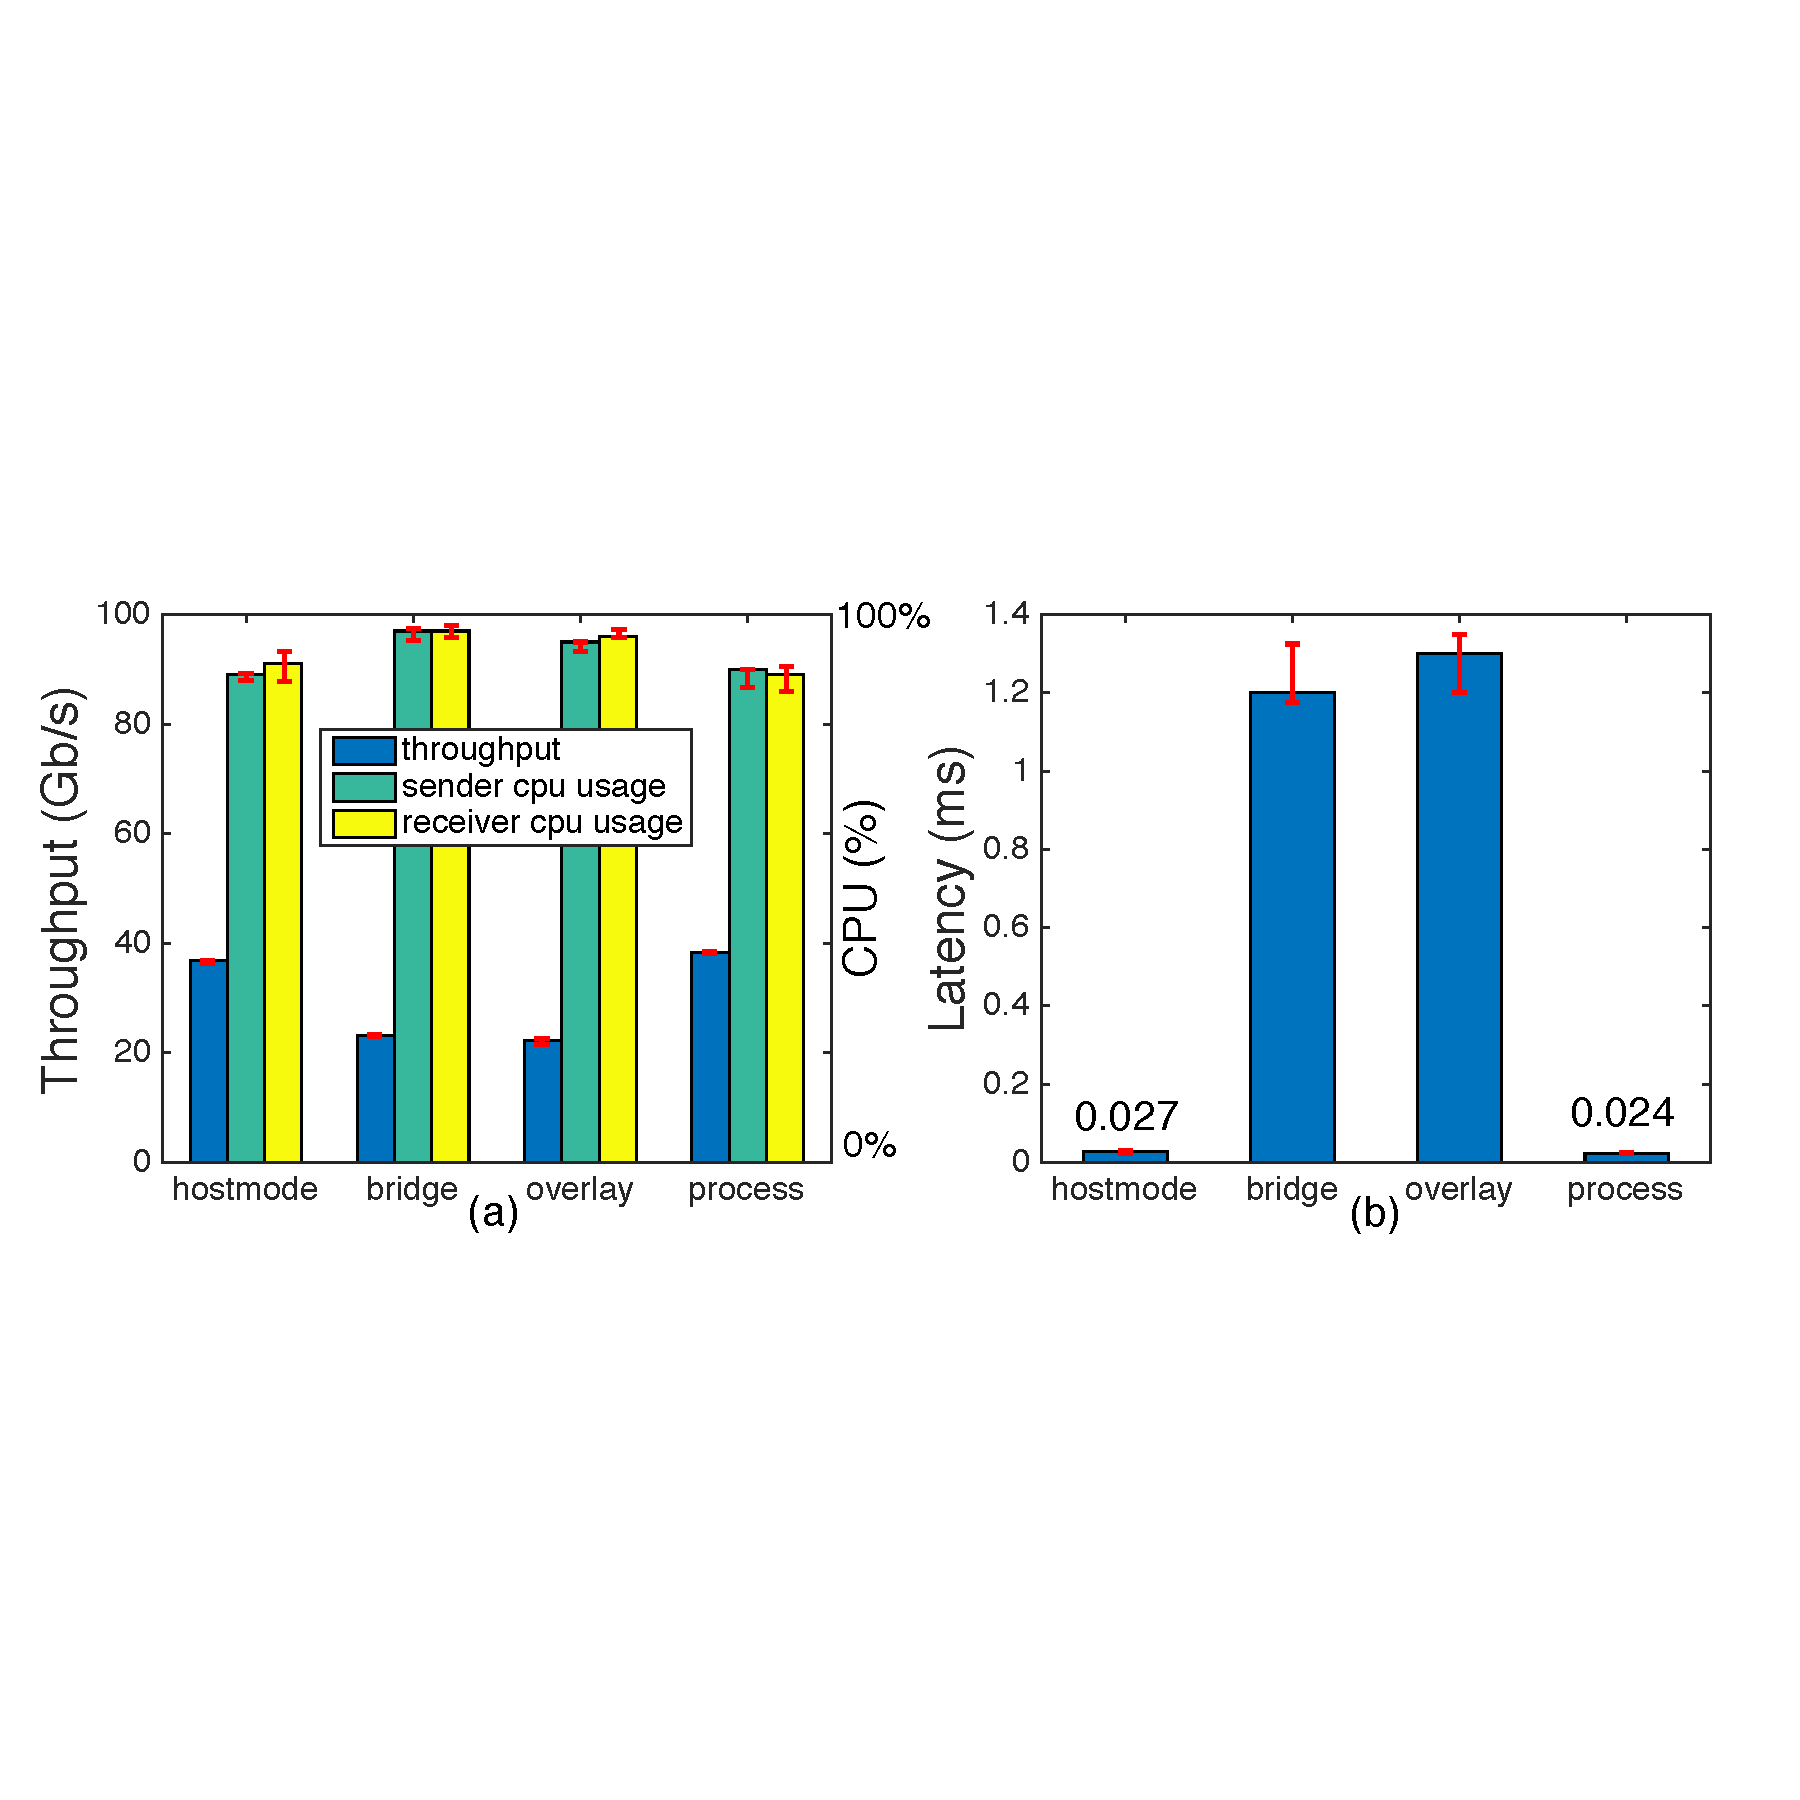
\includegraphics[width=0.5\textwidth]{figures/intro/intro_exist2.pdf} 
     \caption{Performance of two modes of container networking, compared to
     shared memory IPC.} 
     \label{fig:three_modes} 
\end{figure} 
 Unfortunately, containers too suffer the veritable curse of having 
 to sacrifice performance at the expense of isolation and portability. 
 To understand these potential performance bottlenecks, we set up a simple experiment (more details in Section~\ref{sec:motivation}).  
 We set up two Docker containers on a
server (Intel Xeon 2.40GHz 4-cores CPU, 67 GB of memory, 40Gbps Mellanox CX3
NIC, CentOS 7). We consider three ways for the containers to communicate with
each other: (1) {\em Shared Memory:} This requires special setup,
to bypass the namespace isolation, and offers the least isolation, and the least portability;
 (2) {\em Host  mode} 
in which one container binds an interface and a port on the host and use the
host's IP to communicate, like an ordinary process and hence 
 are not truly isolated as they must share the port space; and (3)  {\em Overlay mode} in which the host runs a software
router which connects all containers on the host via  a bridge network and the software routers enable 
 overlay routing across multiple hosts to enable maximum portability as  each container can even have public IPs assigned.
% to
%achieve a uniform IP assignment and traffic routing on the overlay. This makes
%containers fully portable -- they can even have public IPs assigned to them.



%We also had to write a speical application
%that used the shared memory IPC calls for communication. This mode of
%communication offers the least isolation, and the least portability. 

%Next, we considered two networking modes. First, the so-called 
%And then, the so-called 

Figure~\ref{fig:three_modes} is a telling demonstration of the fundamental
tussle between portability, isolation, and performance. We make two
observations from this figure. First, that the throughput and latency of both
modes of inter-container communication is significantly worse than
shared-memory IPC. The reason is obvious: the container communication takes a
``hairpin'' path through the full TCP/IP stack. Second, the performance of
overlay networking is worse than host mode. The reason, again, is simple: in
case of overlay networking, hairpinning happens twice, since the packets must
traverse through the software router as well. This figure thus clearly
illustrates the performance cost of isolation and portability.

As the popularity of container networking grows, this inefficiency must be
addressed. On one hand, the low throughput and high latency directly impacts
the overall performance of large scale distributed systems, such as big data
analytics~\cite{choudhury-paper,mapreduce}, key-value store~\cite{farm,cassandra,bigtable}, machine learning,
etc.  On the other hand, it forces the applications to reserve substantial CPU
resources to merely perform traffic processing, which significantly raise the
cost of running the applications.

One may argue that there is nothing new here: virtualization suffers from
similar inefficiencies and we know how to address them using techniques like
SR-IOV~\cite{sriov} and NetVM~\cite{netvm}. Unfortunately, these ideas cannot be directly applied to the container world.
SR-IOV typically scales to tens of VMs per server. In typical deployments, there
are hundreds of containers per server. The cost of supporting so many containers
in the NIC hardware will be prohibitive.  NetVM~\cite{netvm} cannot be used
directly with containers, since it destroys portability -- it works only when
two VMs are on the same server.  Developers prize containers especially for
their portability: indeed, Docker's main selling point is that a containerized
application that runs on developer's desktop will run in the cloud without any
changes! 

%% In the above experiment, containers were on the same physical server. When
%% containers are on different physical servers, things become even trickier. For
%% example, such containers cannot easily use kernel bypass technologies like RDMA.
%% The reason is subtle: using RDMA (i.e. to bypass the kernel) direct access to
%% NICs is needed. This can only be done in the host mode -- since in the overlay
%% mode, the packets have to pass through the software router.  But operating in
%% the host mode means that containers on the same host share IP address, and must
%% carefully divvy up port space to avoid conflicts.  This limits their portability
%% -- e.g. there can be only one container bound to port 80 on each physical
%% server!

In this paper we outline a solution to address this issue.  Our ultimate vision
is to develop a container networking solution which provides high throughput,
low latency and negligible overhead and fully preserves container portability in
a manner that is completely transparent to application developers. 

To achieve these seemingly conflicting goals, we observe an opportunity to
leverage two key aspects of typical container deployments: (1) they are
typically managed by a central orchestrator (E.g., Mesos \cite{mesos} \vyas{also add kubernetes or whatever to enure this 
 is not mesos specific}) and (2) are typically
deployed over managed network fabrics (e.g., a public cloud provider). Taking
advantage of these easily available additional bits of information, we sketch a
roadmap for an overlay-based solution  with flexible IP assignment and routing
in control-plane \vyas{why is this necessary} that obtains the relevant
deployment-specific information from the aforementioned container orchestrator
and fabric manager and use this in conjunction with the "right" I/O mechanism
(e.g., shared memory when containers are co-located, vs. RDMA when they are
not). 

While this sounds conceptually simple, there are several architectural
and system design challenges in realizing this vision in practice. In the rest
of the paper, we discuss these challenges and sketch a preliminary design. We
will also present results from an early prototype.

\section{Background and Motivation}
\label{sec:motivation}

In this section, we ...

\subsection{Architecture of containerized applications}

\begin{figure*}[!h]  
	\centering   
	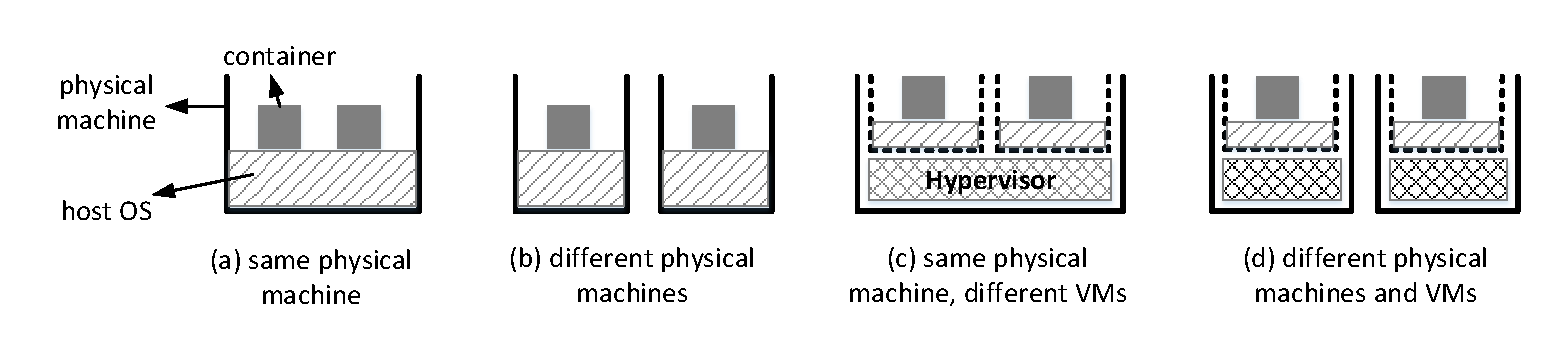
\includegraphics[width=6.7in]{figures/deployment-cases}   
	\caption{\label{fig:deploy-cases} Representative running environments of containers.}   
\end{figure*}   


%\begin{table} [t!]
%\centering
%\small
%\begin{tabular}{ c || c | c | c | c }
%  \hline
%  Constraint & Case (a) & Case (b) & Case (c) & Case (d) \\ \hline \hline
%  N/A & SharedMem & RDMA & SharedMem & RDMA \\ \hline
%  w/o trust & TCP/IP & TCP/IP & TCP/IP & TCP/IP \\ \hline
%  w/o RDMA NIC & SharedMem & TCP/IP & SharedMem & TCP/IP \\ \hline
%\end{tabular}
%\caption{\label{tab:best-network} The suggested network solution under %different running environments in Figure~\ref{fig:deploy-cases} and constraints.}
%\normalsize
%\end{table}

Nowadays, a containerized application is usually composed by multiple containers. For example, each master and slave node in Hadoop is an individual container; A web service can include layers, such as load balancer, web server,
in-memory cache and backend database, and each layer can be a distributed 
system with multiple containerized nodes. 
These containers are usually 
deployed into a multi-host server cluster, and the deployment is usually 
controlled by a cluster orchestrator, e.g. Mesos~\cite{?}. 
Such architecture makes it easier
to upgrade the nodes or mitigate failures, since a stopped container can be quickly replaced by a new one on the same or another host.

Working as a single application, containers need to exchange data, and the network performance has a huge impact on the overall application performance.
Depending on whether 
containers run on bare-metal hosts or VM hosts, Figure~\ref{fig:deploy-cases}
illustrates four representative cases for a container networking solutions
to handle. 
%As shown later in this section, one networking solution has 
%different efficiency and feasibility in different cases. 
In this paper, 
we focus on the first two cases and discuss how to support the second two
in the future.


\subsection{Existing Solutions of Container Networking}

P1: [Details and related work for existing container network solutions]There are two networking modes to inter-connect containers over multiple hosts:

\begin{itemize}
  \item Host mode: breaking the portability and independency
  \item Overlay mode: keeping the portability and independency
  \begin{itemize}
  \item Docker native overlay
  \item Weave
  \item Caliber (Optional)
  \end{itemize}  
\end{itemize}


Conclusions:
\begin{itemize}
  \item The intra-host throughput of existing solutions are less than 40Gb/s.
  \item The throughput, latency of two containers with host mode is close to the throughput of processes.
  \item All the existing solutions put a heavy load on CPU. CPU is the main bottleneck for throughput.
\end{itemize}

\subsection{Opportunities to build a better container networks}
P1: [Comparing container networking with other solutions]: In Sec 1, we have already seen the poor performance and high overhead of current container networking solution. Given containers are essentially processes, there are multiple better ways for two containers to communicate with each other.

\begin{itemize}
  \item Shared memory
  \item RDMA
  \item DPDK (not sure whether we have time to do it)
\end{itemize}

\subsubsection{Intra-host communication}

Throughput:
     \begin{figure}[ht]
     \centering 
     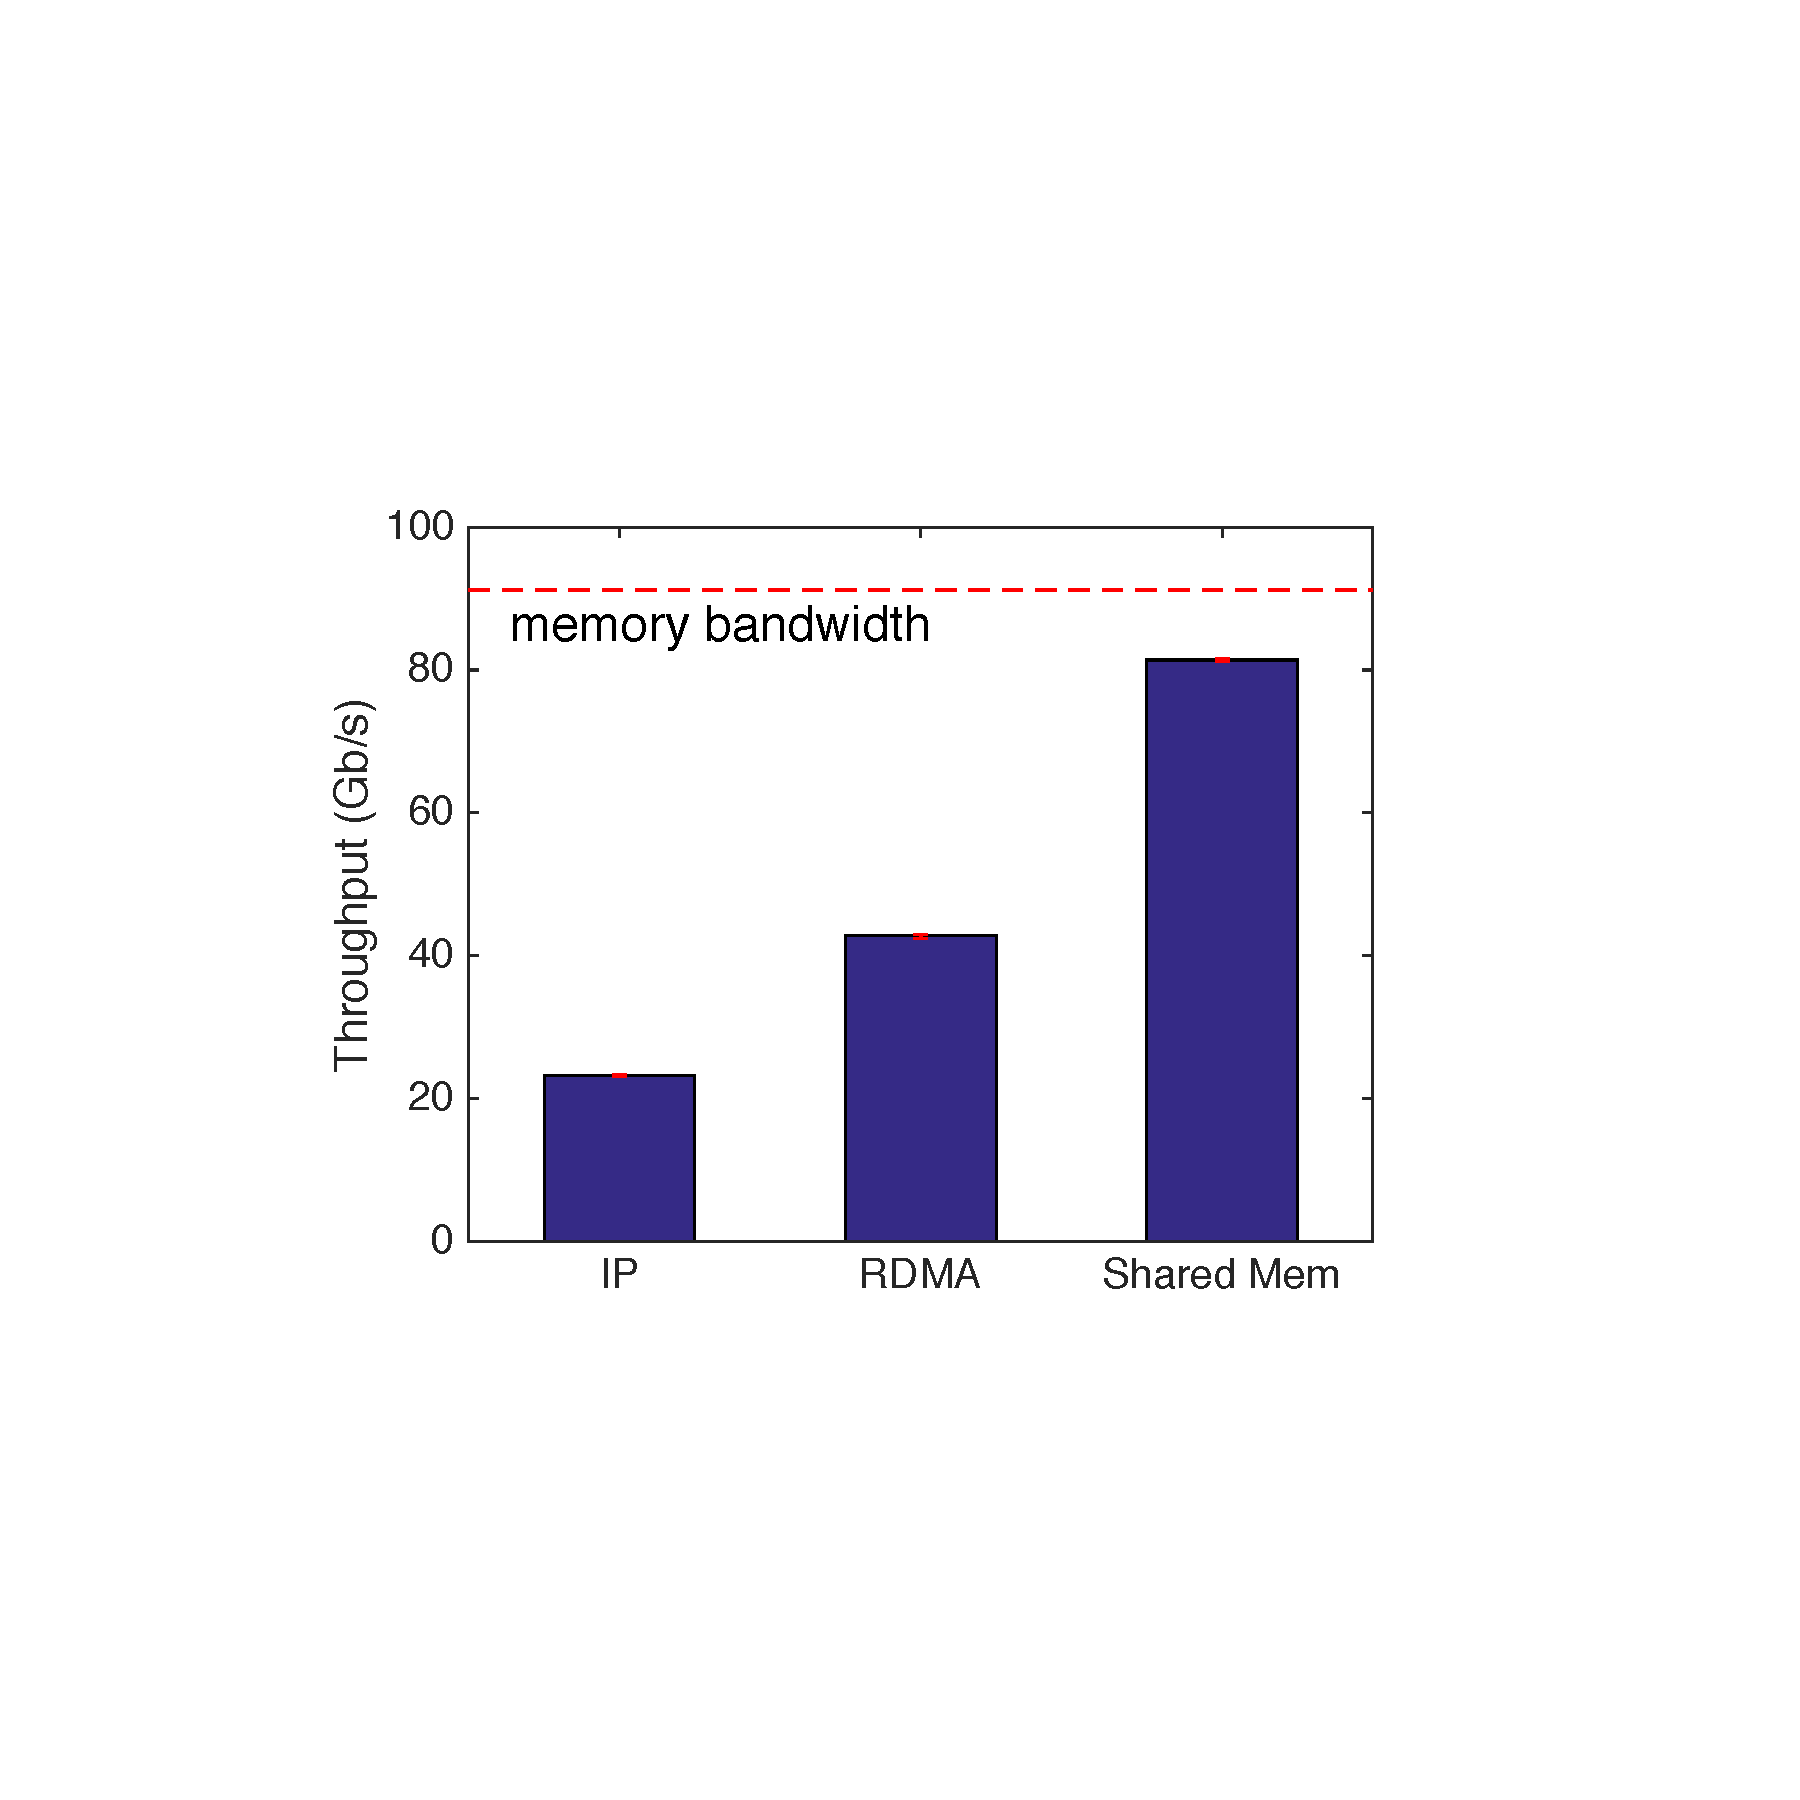
\includegraphics[width=0.32\textwidth]{figures/motivation/eval_baremetal_thr.pdf}      
     \label{fig:eval_baremetal_thr}
     \caption{} 
     \end{figure}

Latency:    
     \begin{figure}[ht]
     \centering 
     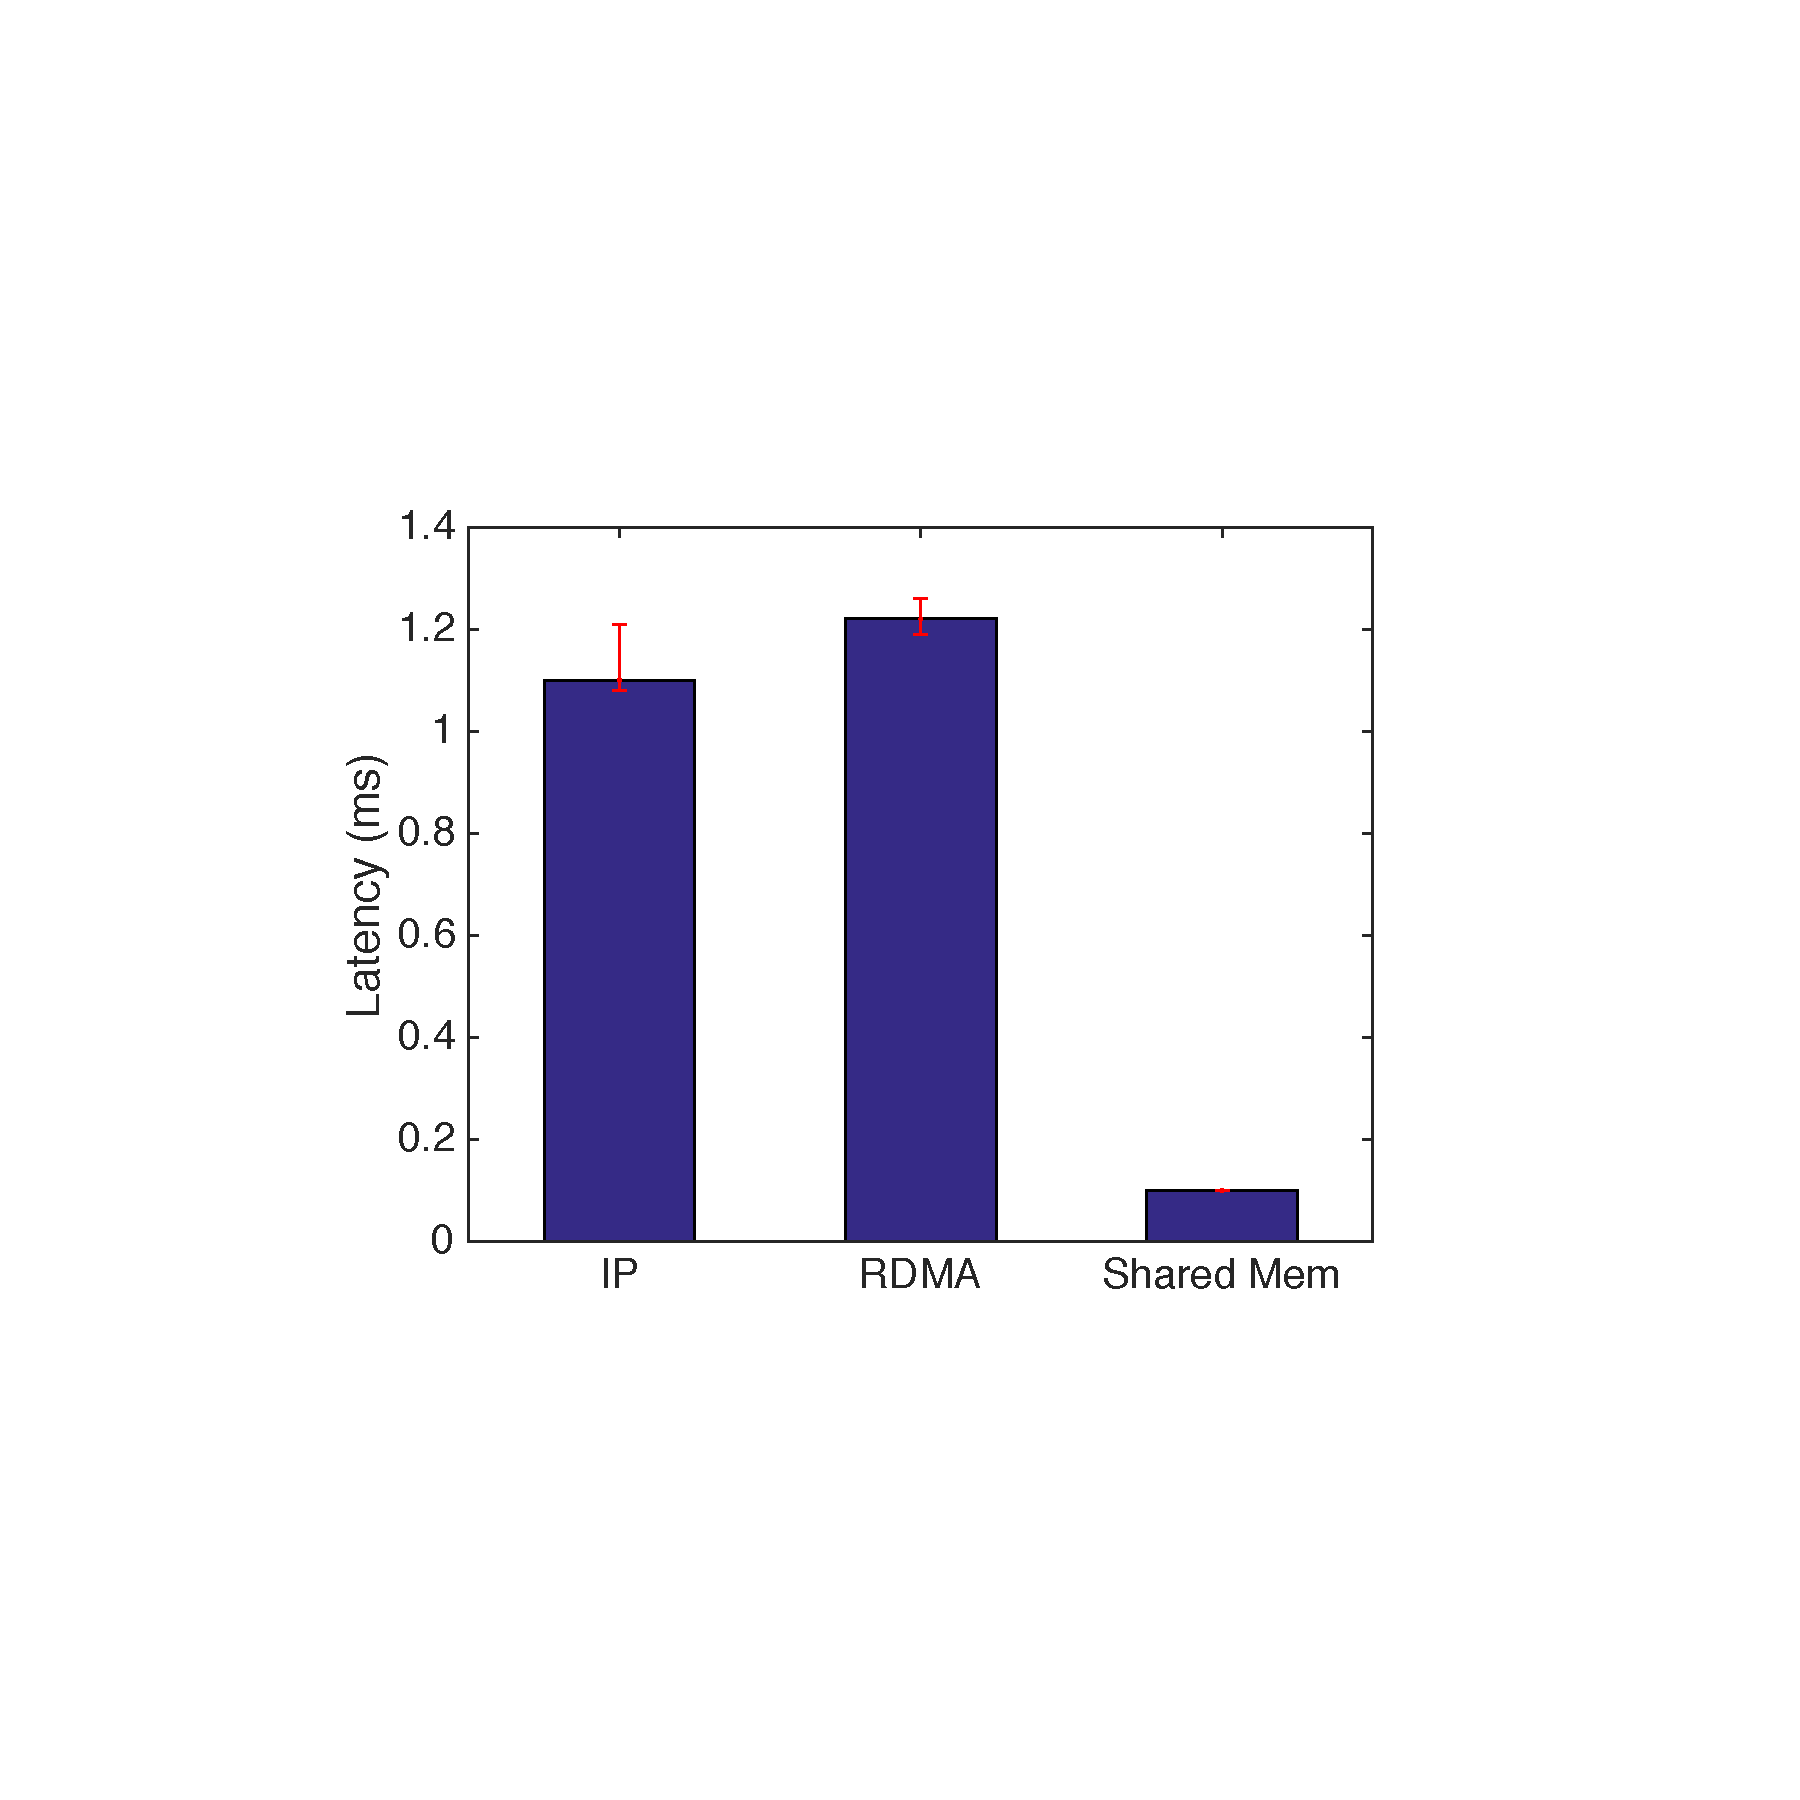
\includegraphics[width=0.32\textwidth]{figures/motivation/eval_baremetal_latency.pdf}      
     \label{fig:eval_baremetal_latency}
     \caption{} 
     \end{figure}

CPU usage:     
     \begin{figure}[ht]
     \centering 
     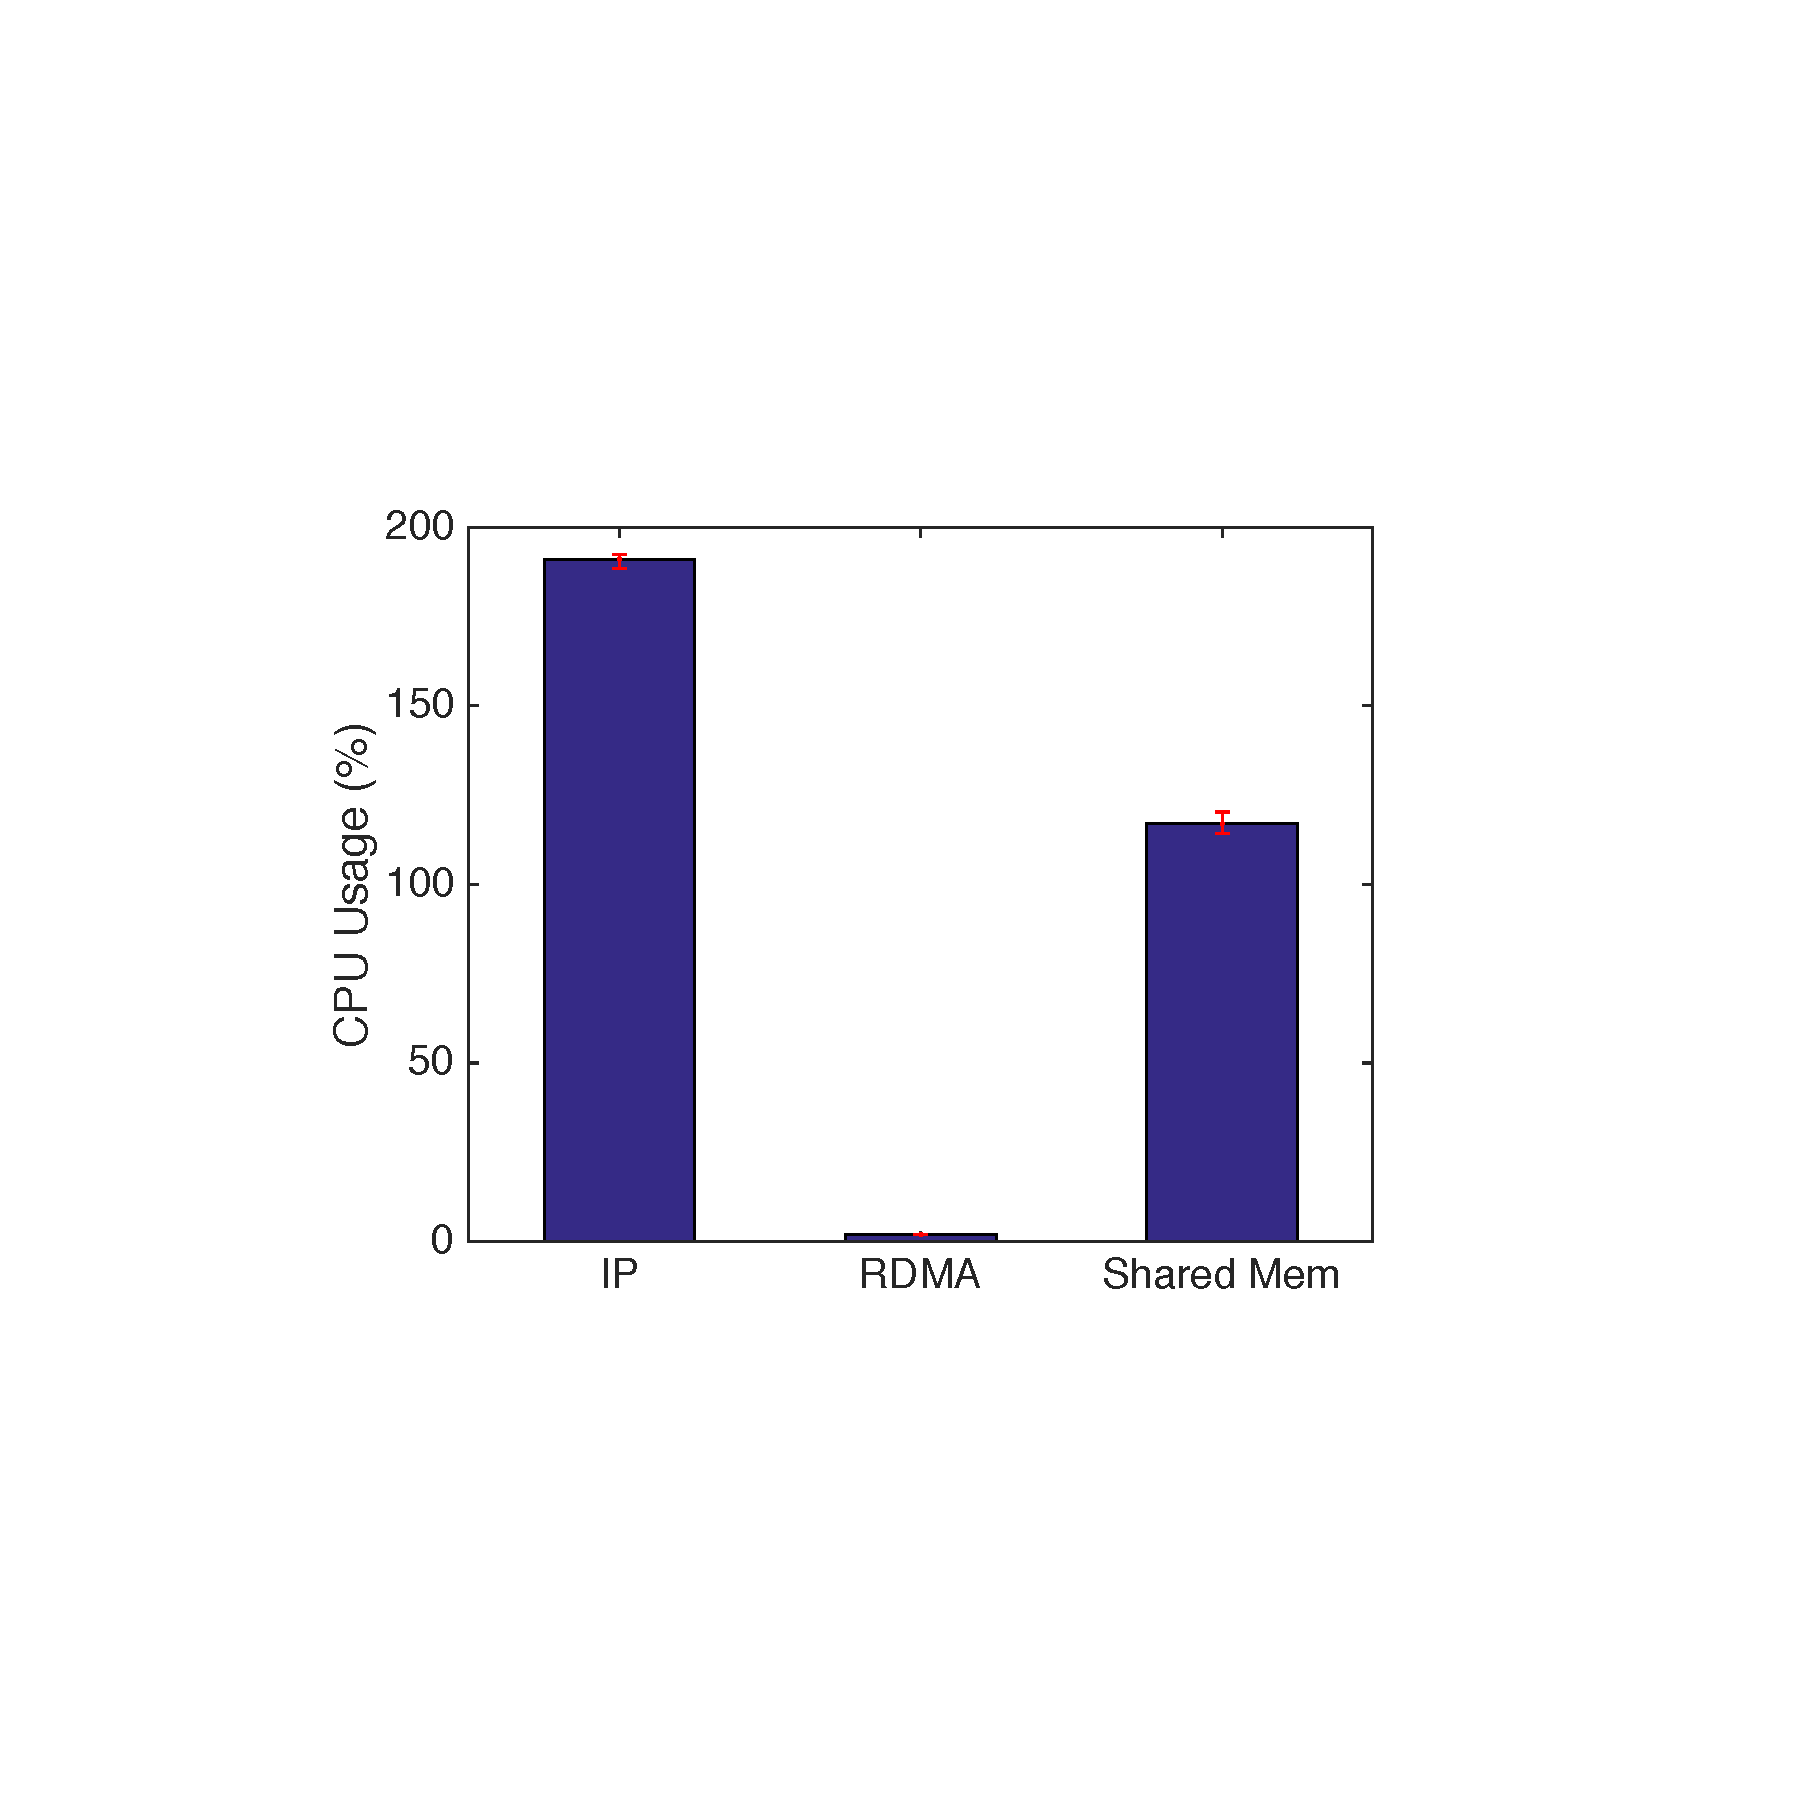
\includegraphics[width=0.32\textwidth]{figures/motivation/eval_baremetal_cpu.pdf}      
     \label{fig:eval_baremetal_cpu}
     \caption{} 
     \end{figure}
     
\begin{itemize}
  \item Communication via bridge mode only achieves 27Gb/s throughput, 1 ms latency but uses near to 200\% of cpu. (Host mode and overlay mode are similar.)
  \item RDMA only improves the throughput to 40Gb/s for containers on the same machine, the latency is still 1ms, though it has a low cpu usage.
  \item Shared memory can achieve near-to-memory-bandwidth throughput, lowest latency, but still burns some cpu. 
\end{itemize}


\subsubsection{Inter-host communication}


\subsection{Our Goals}
P1: [Goal] We want to build a container overlay networking solution which can guarantee the best network performance while keeping portability and independency for containers.

P2: [Specific requirements, challenges]
\begin{itemize}
  \item Smartly choosing network solutions (e.g. shared- memory, RDMA, DPDK, etc.) according to multiple factors.
  \item Making the network solution selection and switching be transparent to containers.
  \item IP assignments is independent to container's locations.
\end{itemize}

%%% commented content 
\iffalse

\begin{figure}[ht]
     \centering 
     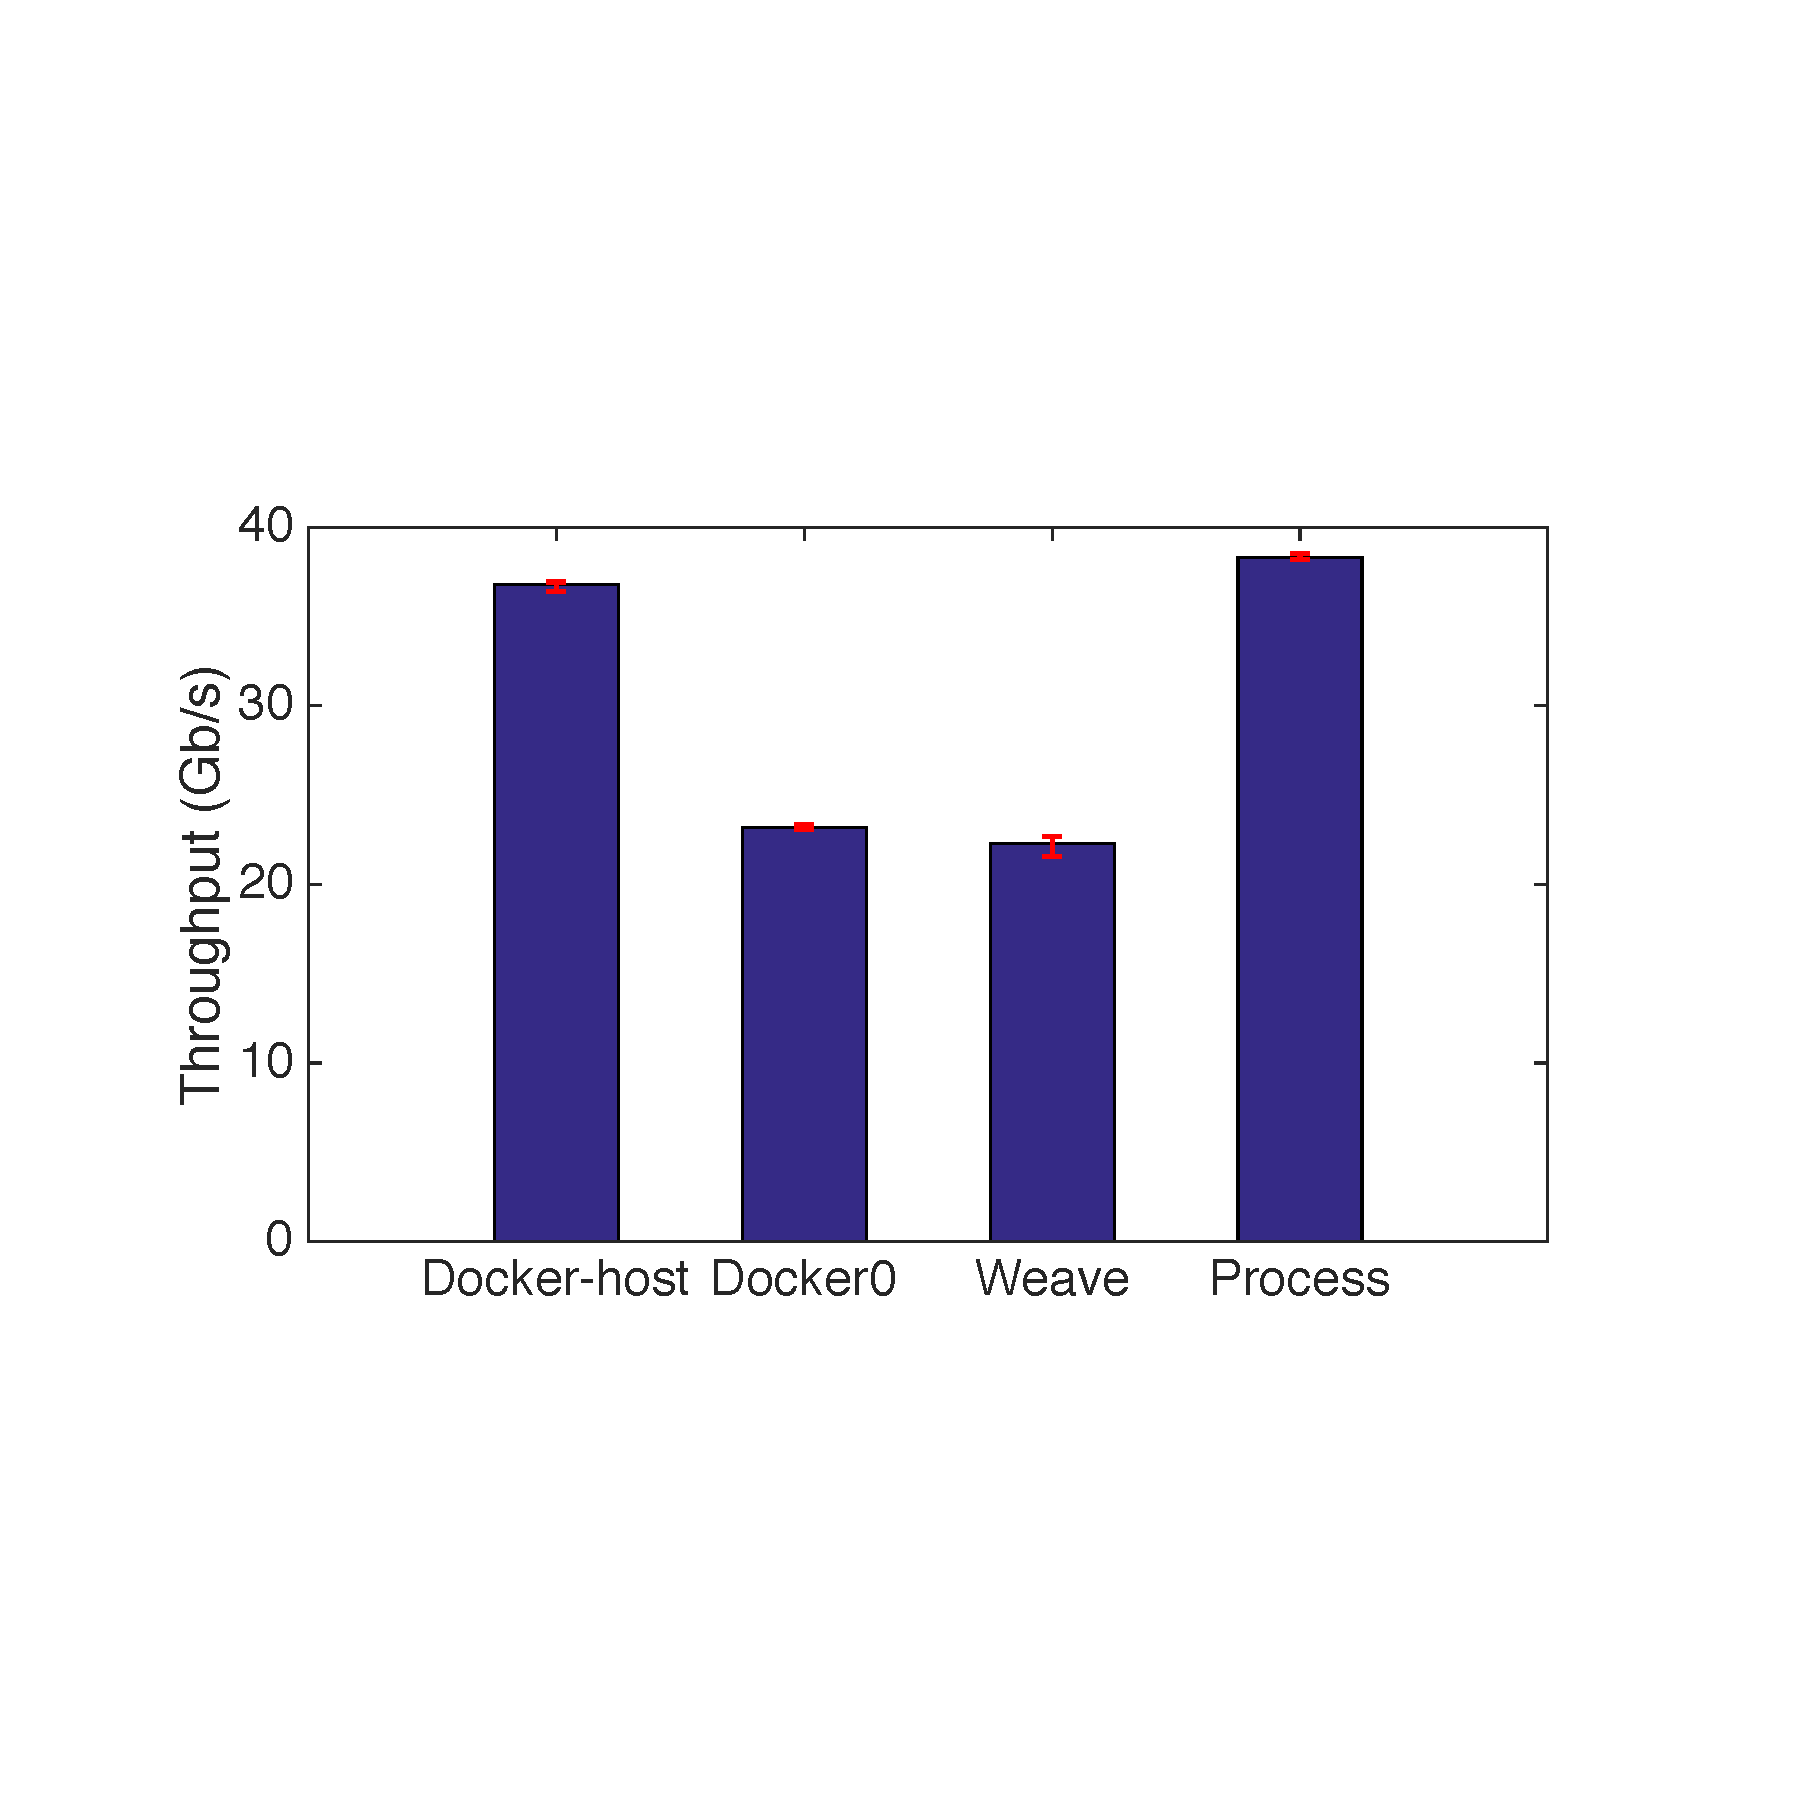
\includegraphics[width=0.4\textwidth]{figures/motivation/eval_exist_bw.pdf} 
     \label{fig:eval_exist_bw}
     \caption{The intra-host throughput of existing solutions. Docker-host is in host mode; Docker0 is in bridge mode; Weave is in overlay mode.} 
\end{figure} 

\begin{figure}[ht]
     \centering 
     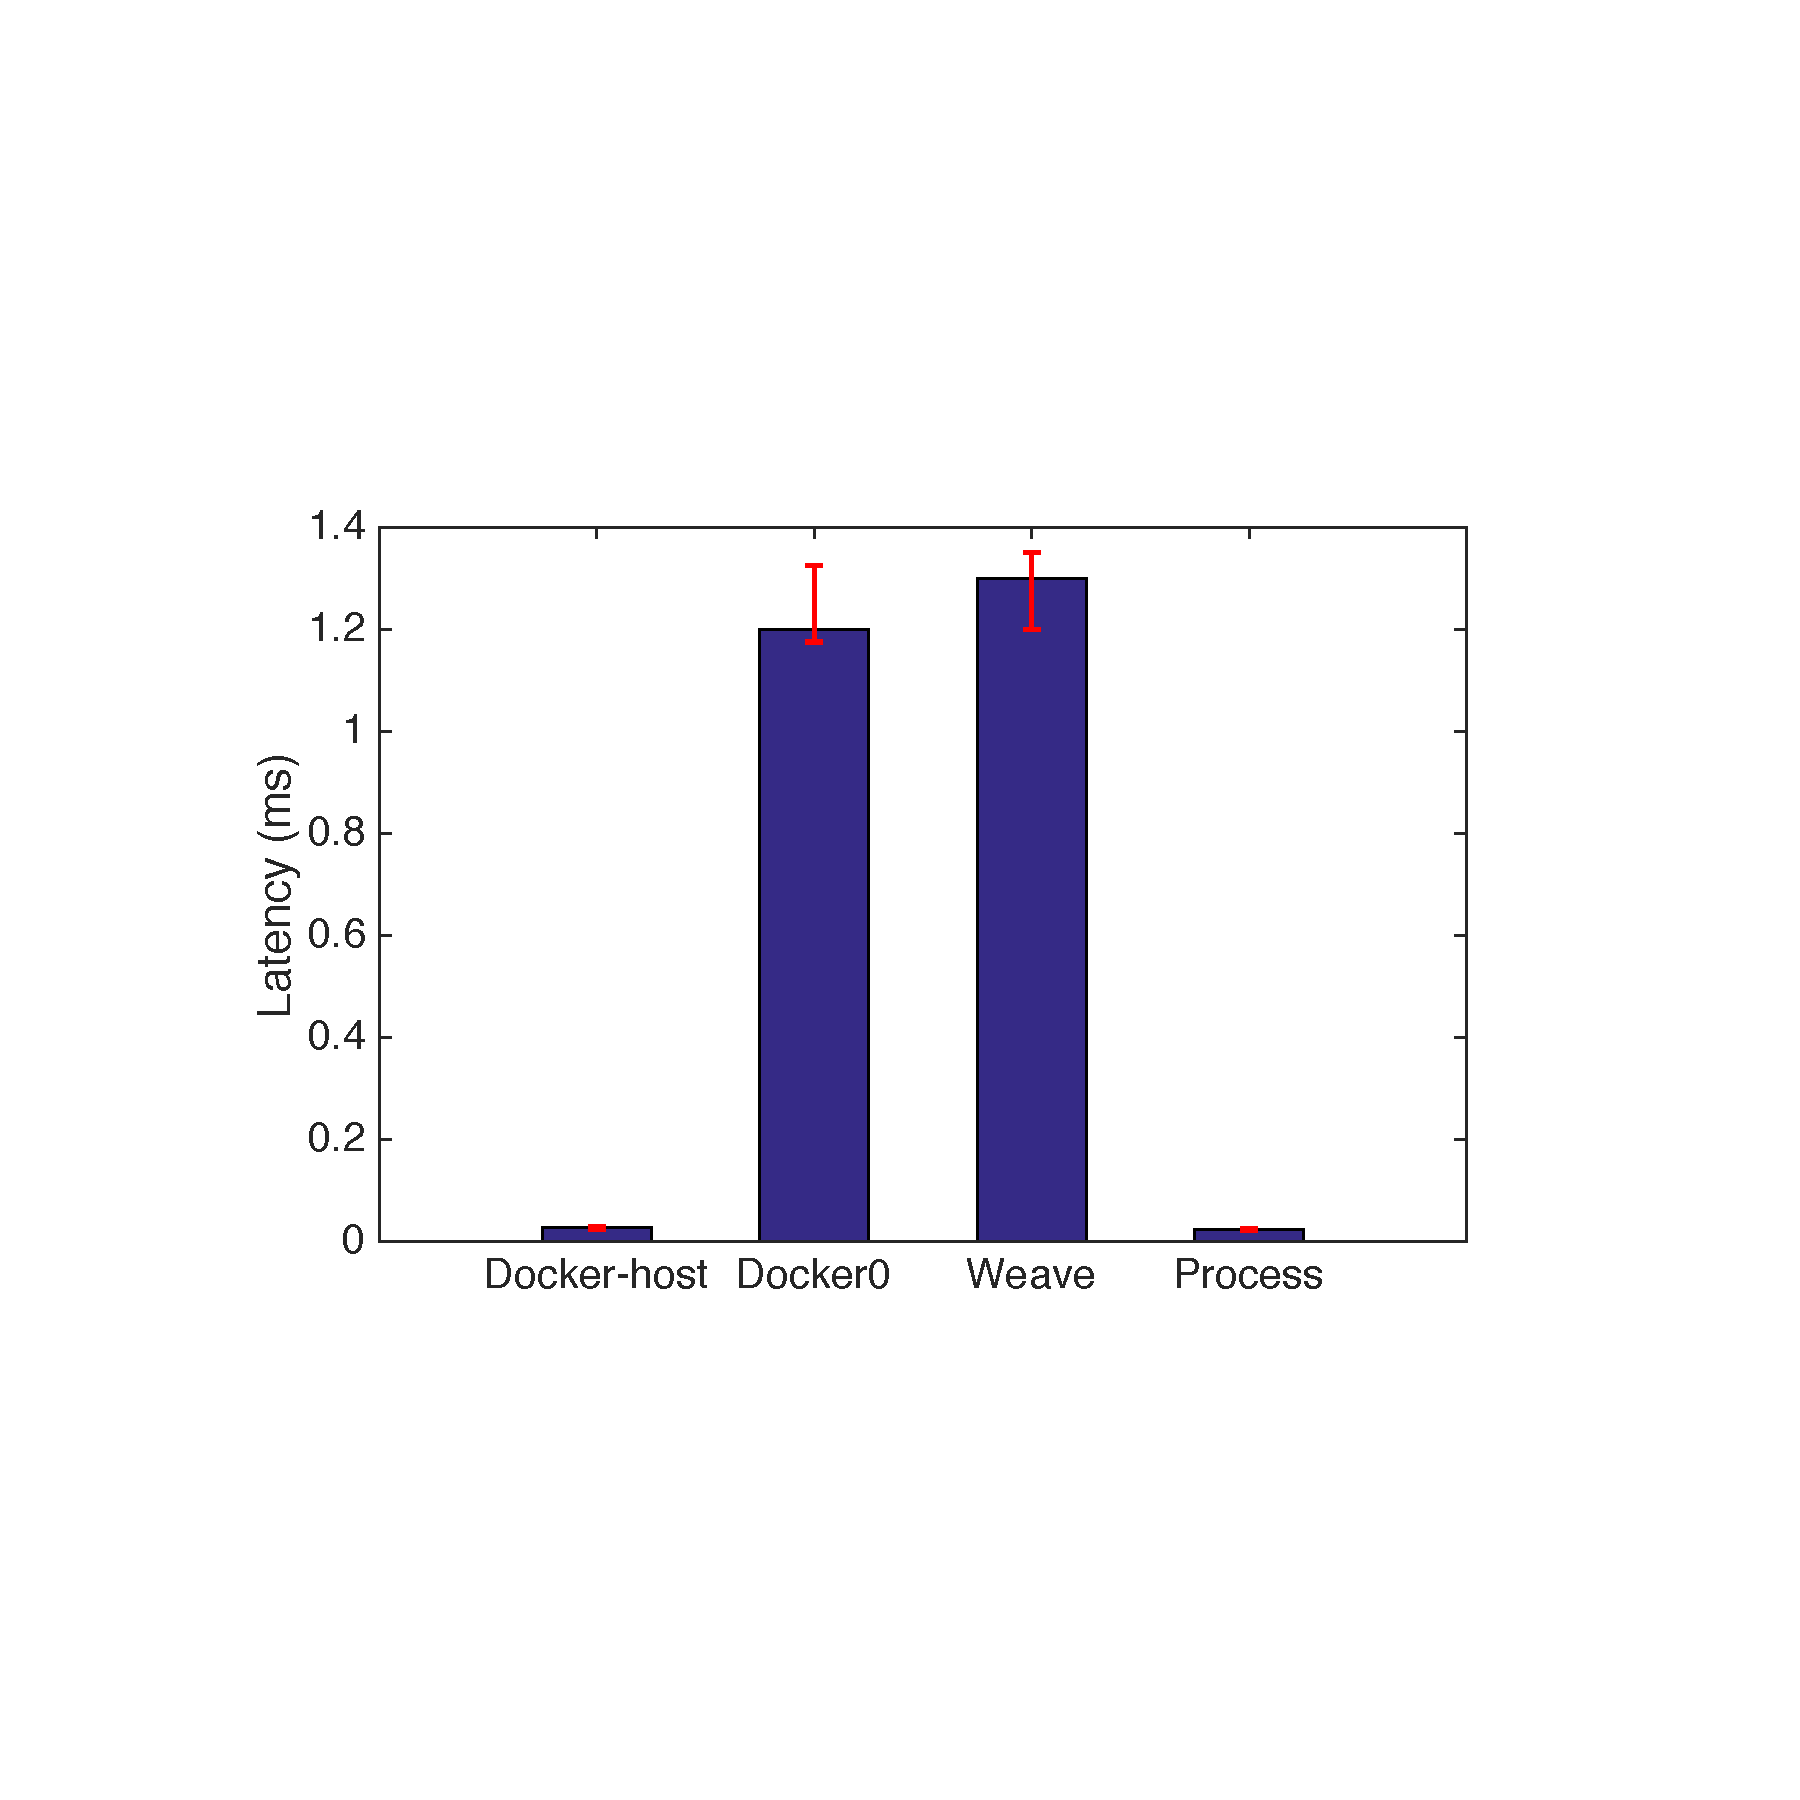
\includegraphics[width=0.4\textwidth]{figures/motivation/eval_exist_latency.pdf} 
     \label{fig:eval_exist_latency}
     \caption{The intra-host latency of existing solutions. Docker-host is in host mode; Docker0 is in bridge mode; Weave is in overlay mode.} 
\end{figure} 

\begin{figure}[ht]
     \centering 
     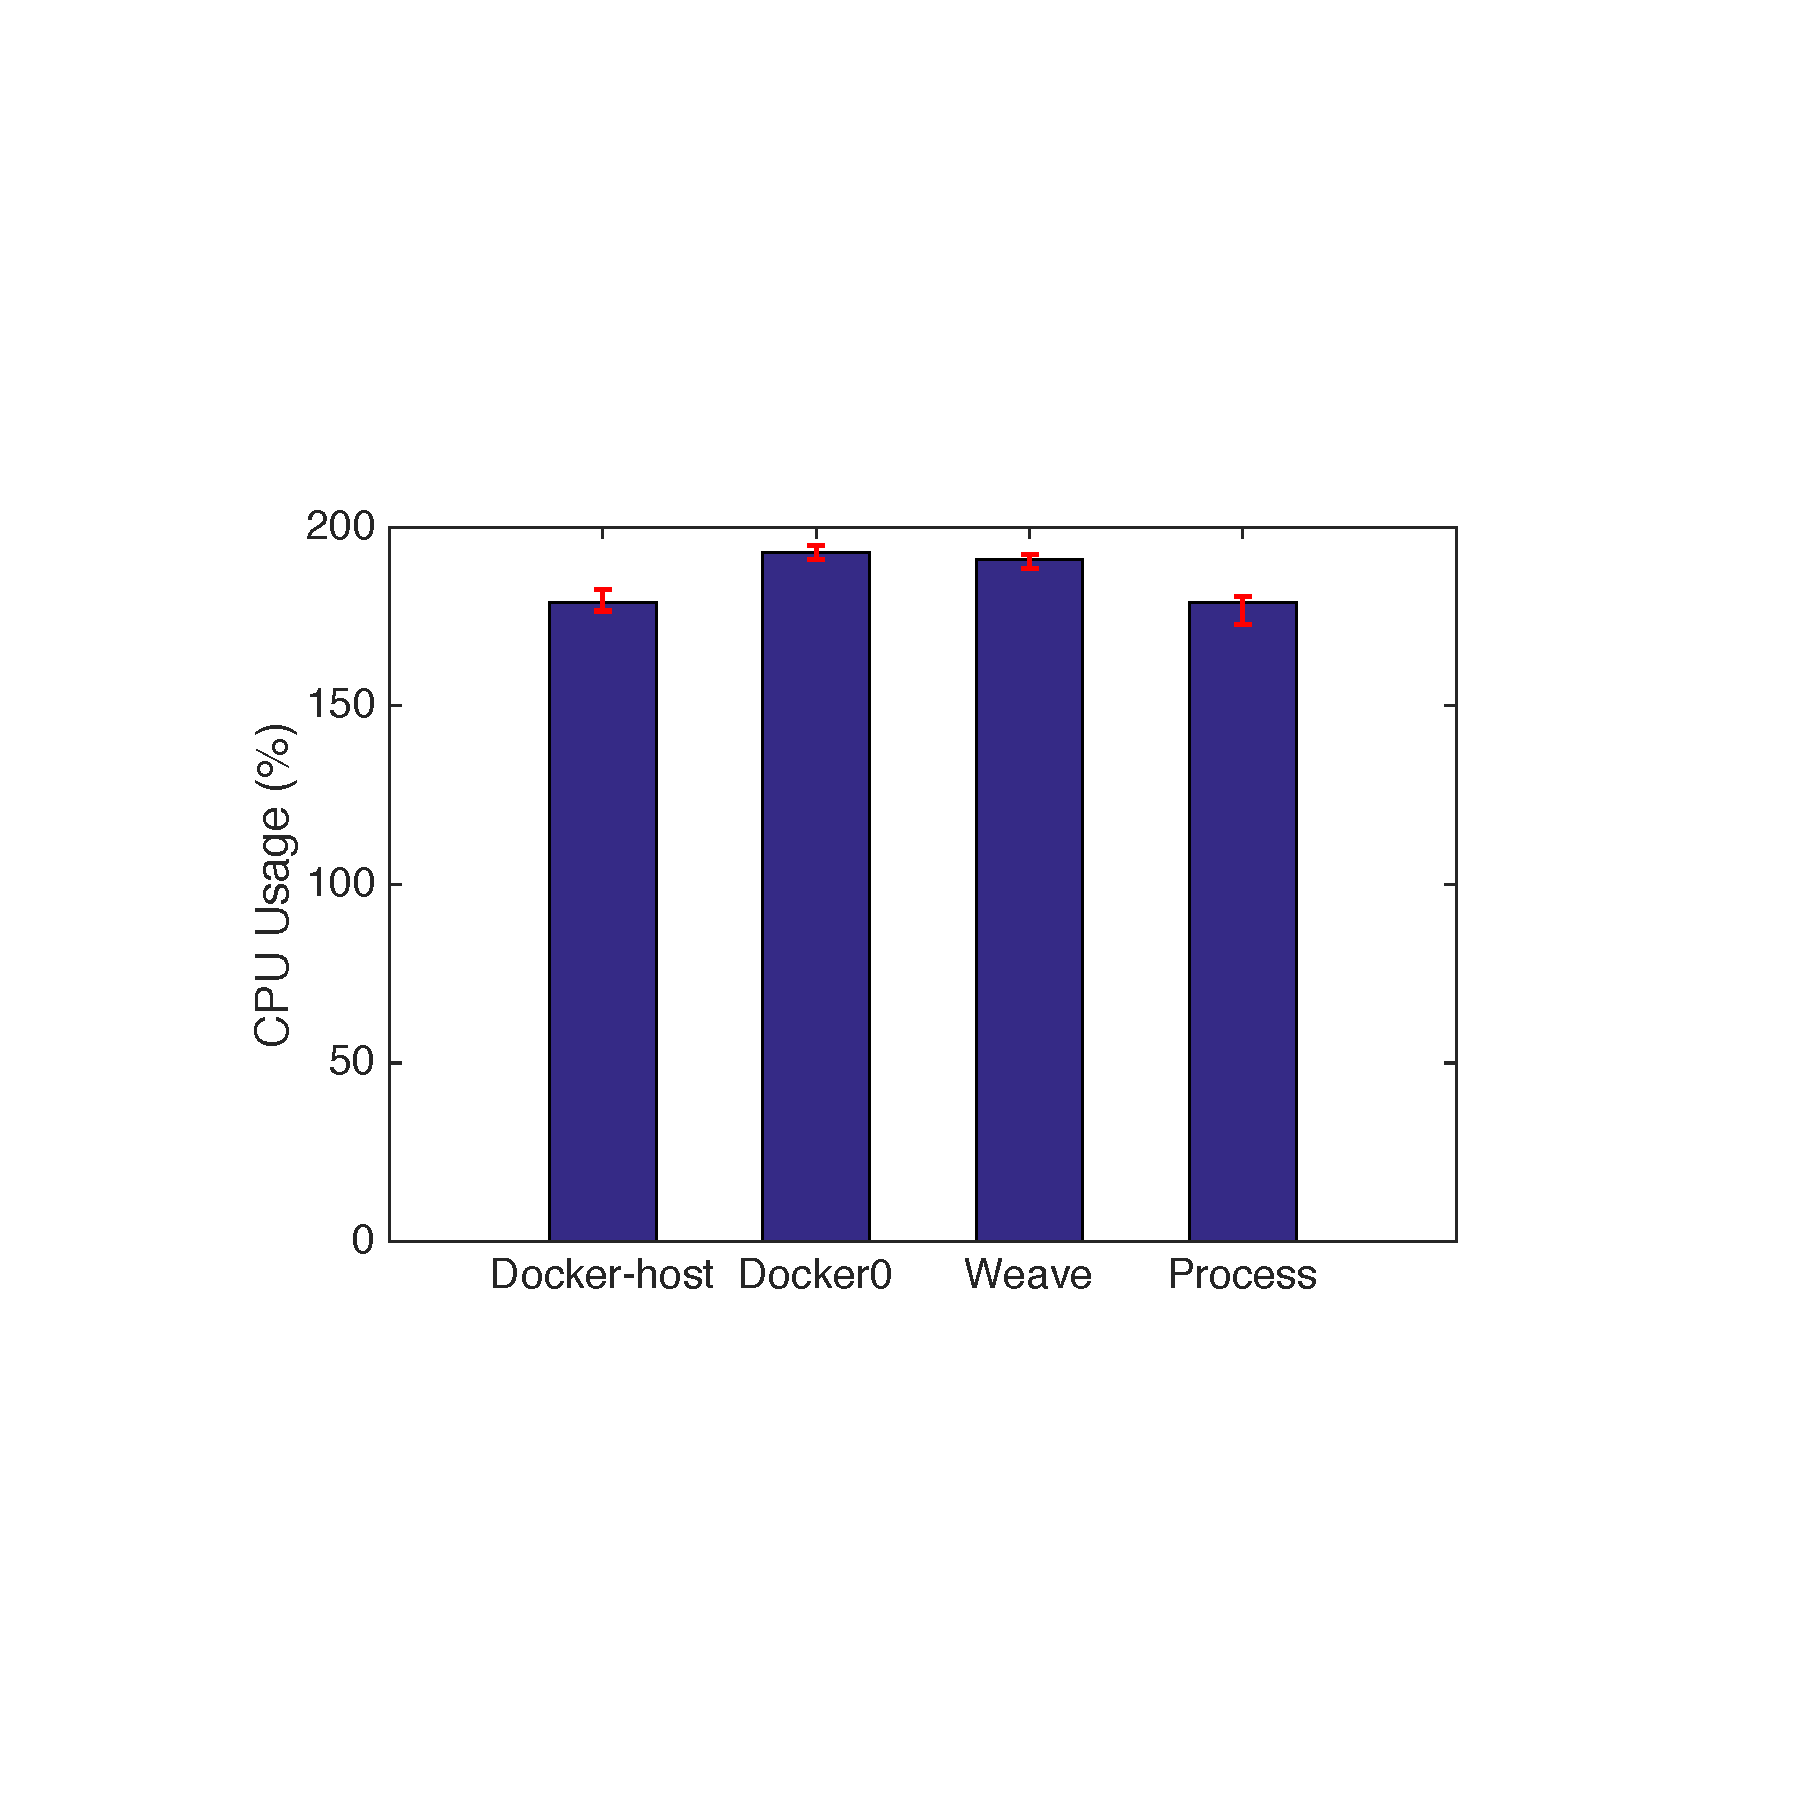
\includegraphics[width=0.4\textwidth]{figures/motivation/eval_exist_cpu.pdf} 
     \label{fig:eval_exist_cpu}
     \caption{The cpu usage of existing solutions. Docker-host is in host mode; Docker0 is in bridge mode; Weave is in overlay mode.} 
\end{figure} 

\begin{figure}[ht]
     \centering 
     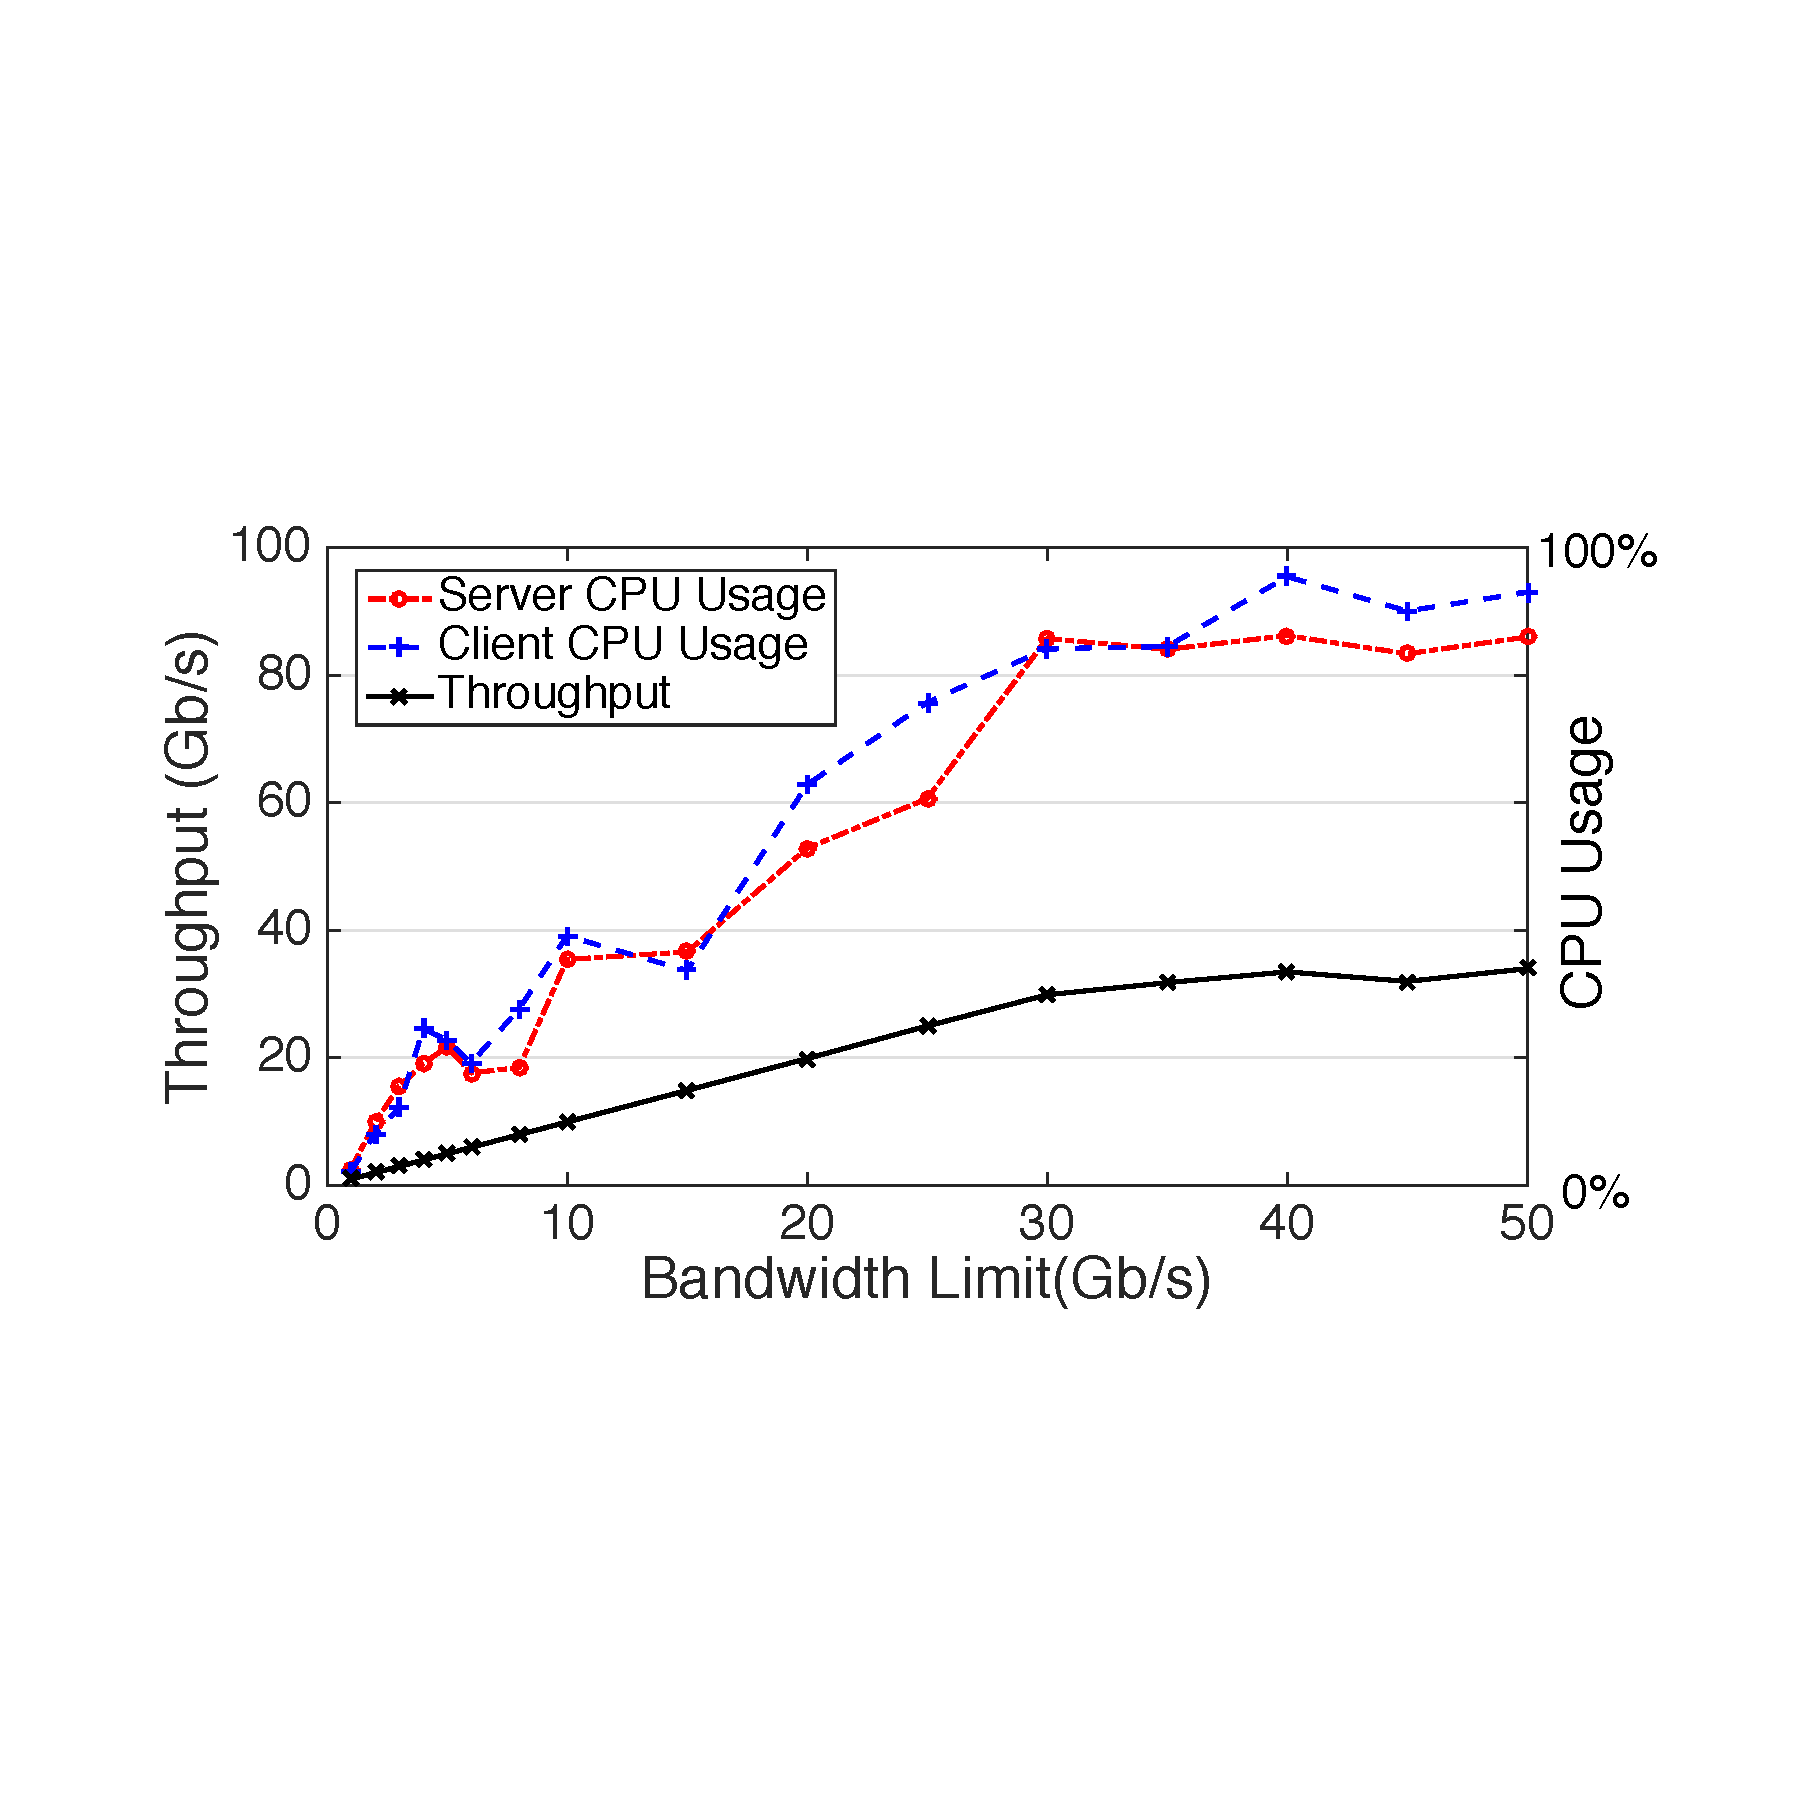
\includegraphics[width=0.4\textwidth]{figures/motivation/eval_bw_cpu.pdf}      
     \label{fig:eval_bw_cpu}
     \caption{} 
\end{figure}


* Figures:

* Throughput comparison (intra- and inter-host)

* CPU comparison

* Latency comparison

In this section, we present measurement results that demonstrates the network performance and resource overhead of different optional network channels. We focus on network throughput and latency when containers are located in the same or different hosts. 


\subsection{Existing container networking solutions}

A bridge is a way to connect two Ethernet segments together in a protocol independent way. Packets are forwarded based on Ethernet address, rather than IP address (like a router). Since forwarding is done at Layer 2, all protocols can go transparently through a bridge.

The Linux bridge code implements a subset of the ANSI/IEEE 802.1d standard. [1]. The original Linux bridging was first done in Linux 2.2, then rewritten by Lennert Buytenhek. The code for bridging has been integrated into 2.4 and 2.6 kernel series.


\subsection{Opportunities}

\subsection{Challenges}

\subsection{The ineffiencies in container networking}

We measure the throughput and latency of TCP/IP, Shared-Mem and RDMA under cases
(a) (b) (c) and (d).

\harry{RDMA and Shared-Mem is missing under (c) and (d)}.

\para{The measurement setup}
(1) two bare metals: 40Gbps NICs.
(2) two VMs on top of the two bare metals.
(3) two VMs from Azure or EC2.

\subsection{Intra-host performance}
\subsubsection{throughput vs. latency vs. cpu usage}

\begin{figure*}[t]
     \centering 
     %\begin{subfigure}[t]{0.25\textwidth}
     \begin{subfigure}[t]
     \centering 
     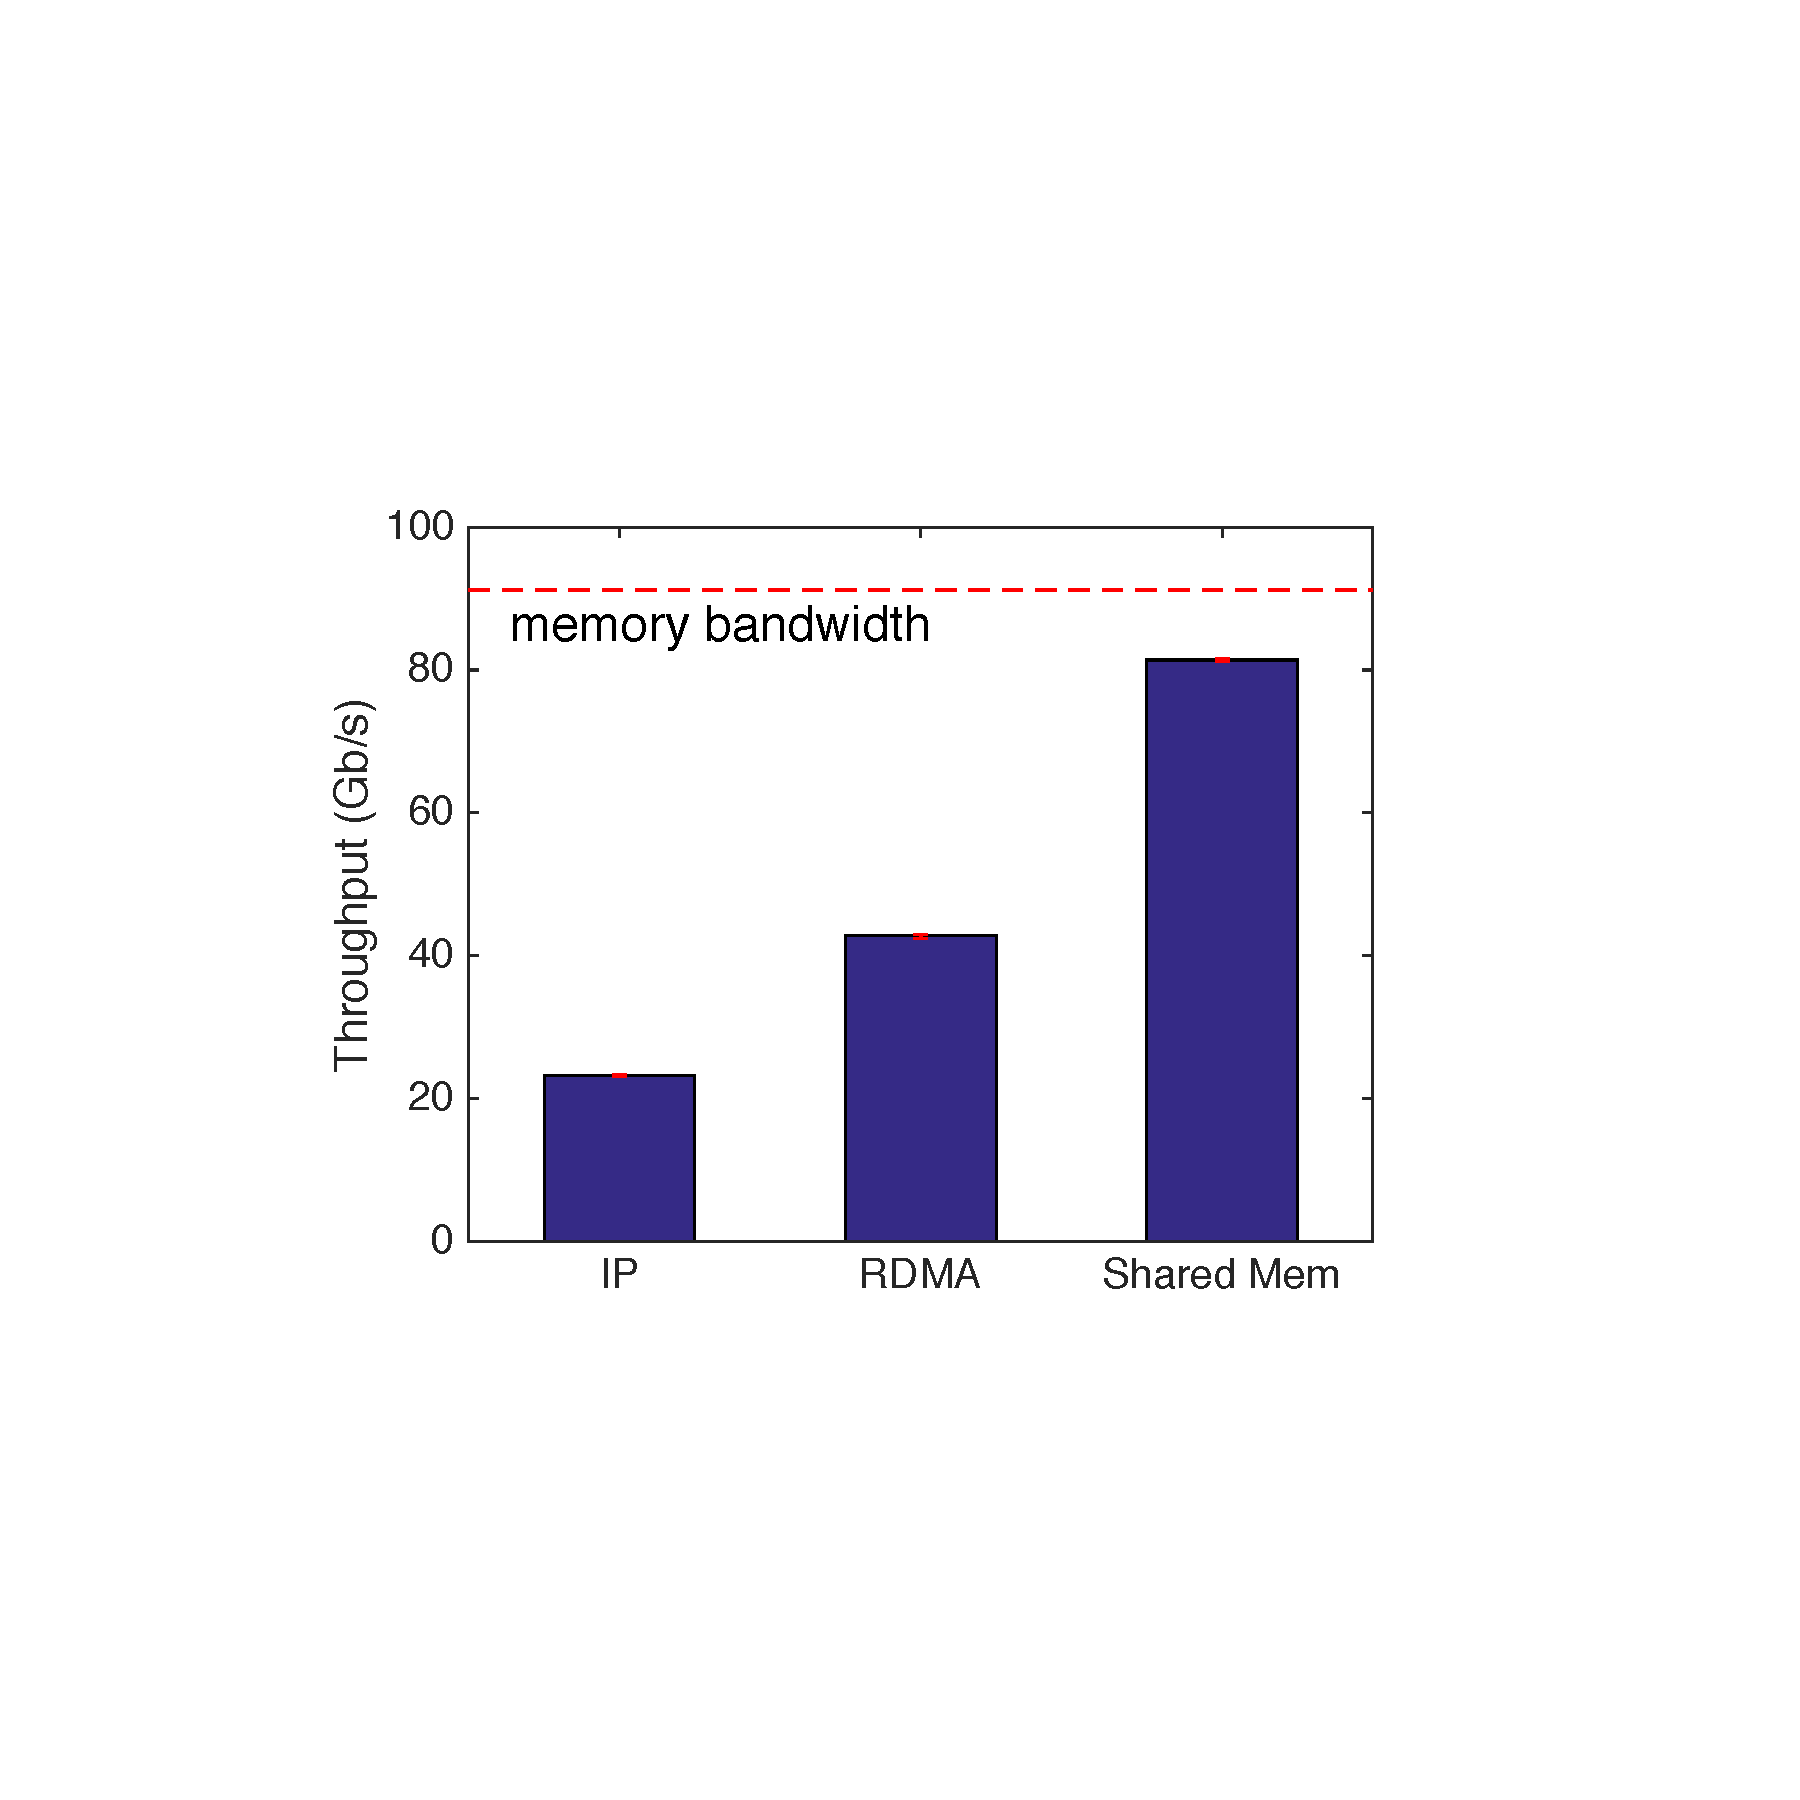
\includegraphics[width=0.32\textwidth]{figures/motivation/eval_baremetal_thr.pdf}      
     %\label{fig:eval_baremetal_thr}
     %\caption{} 
     \end{subfigure}      
     \begin{subfigure}[t]
     \centering 
     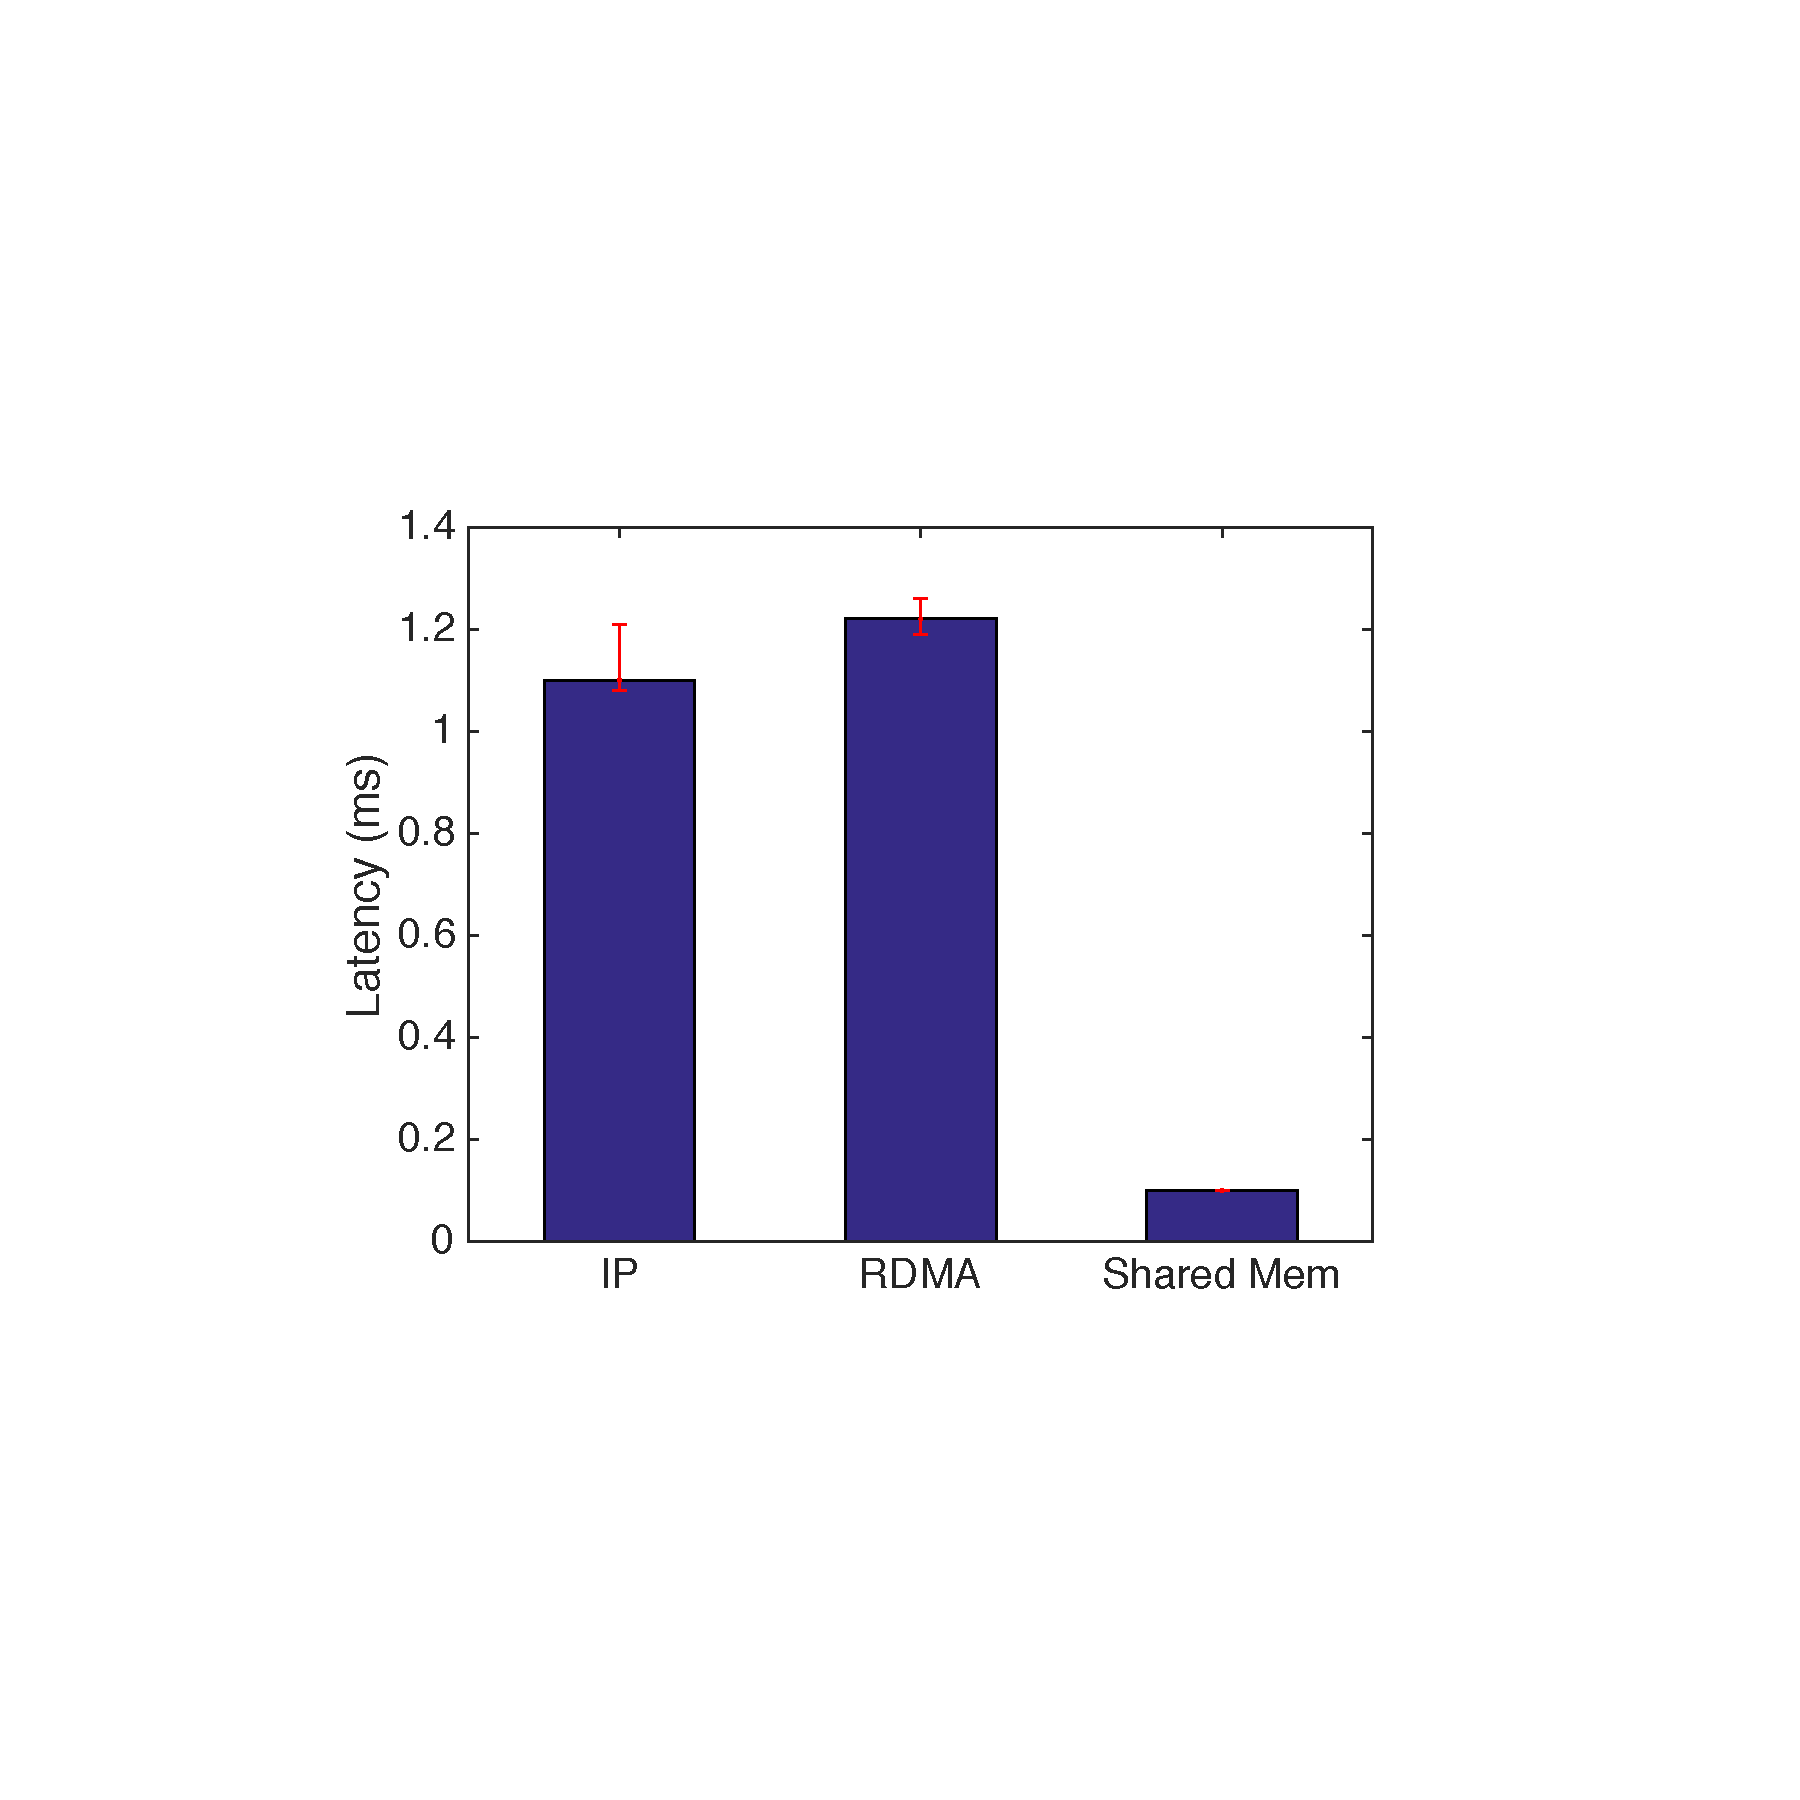
\includegraphics[width=0.32\textwidth]{figures/motivation/eval_baremetal_latency.pdf}      
     %\label{fig:eval_baremetal_latency}
     %\caption{} 
     \end{subfigure}      
     \begin{subfigure}[t]
     \centering 
     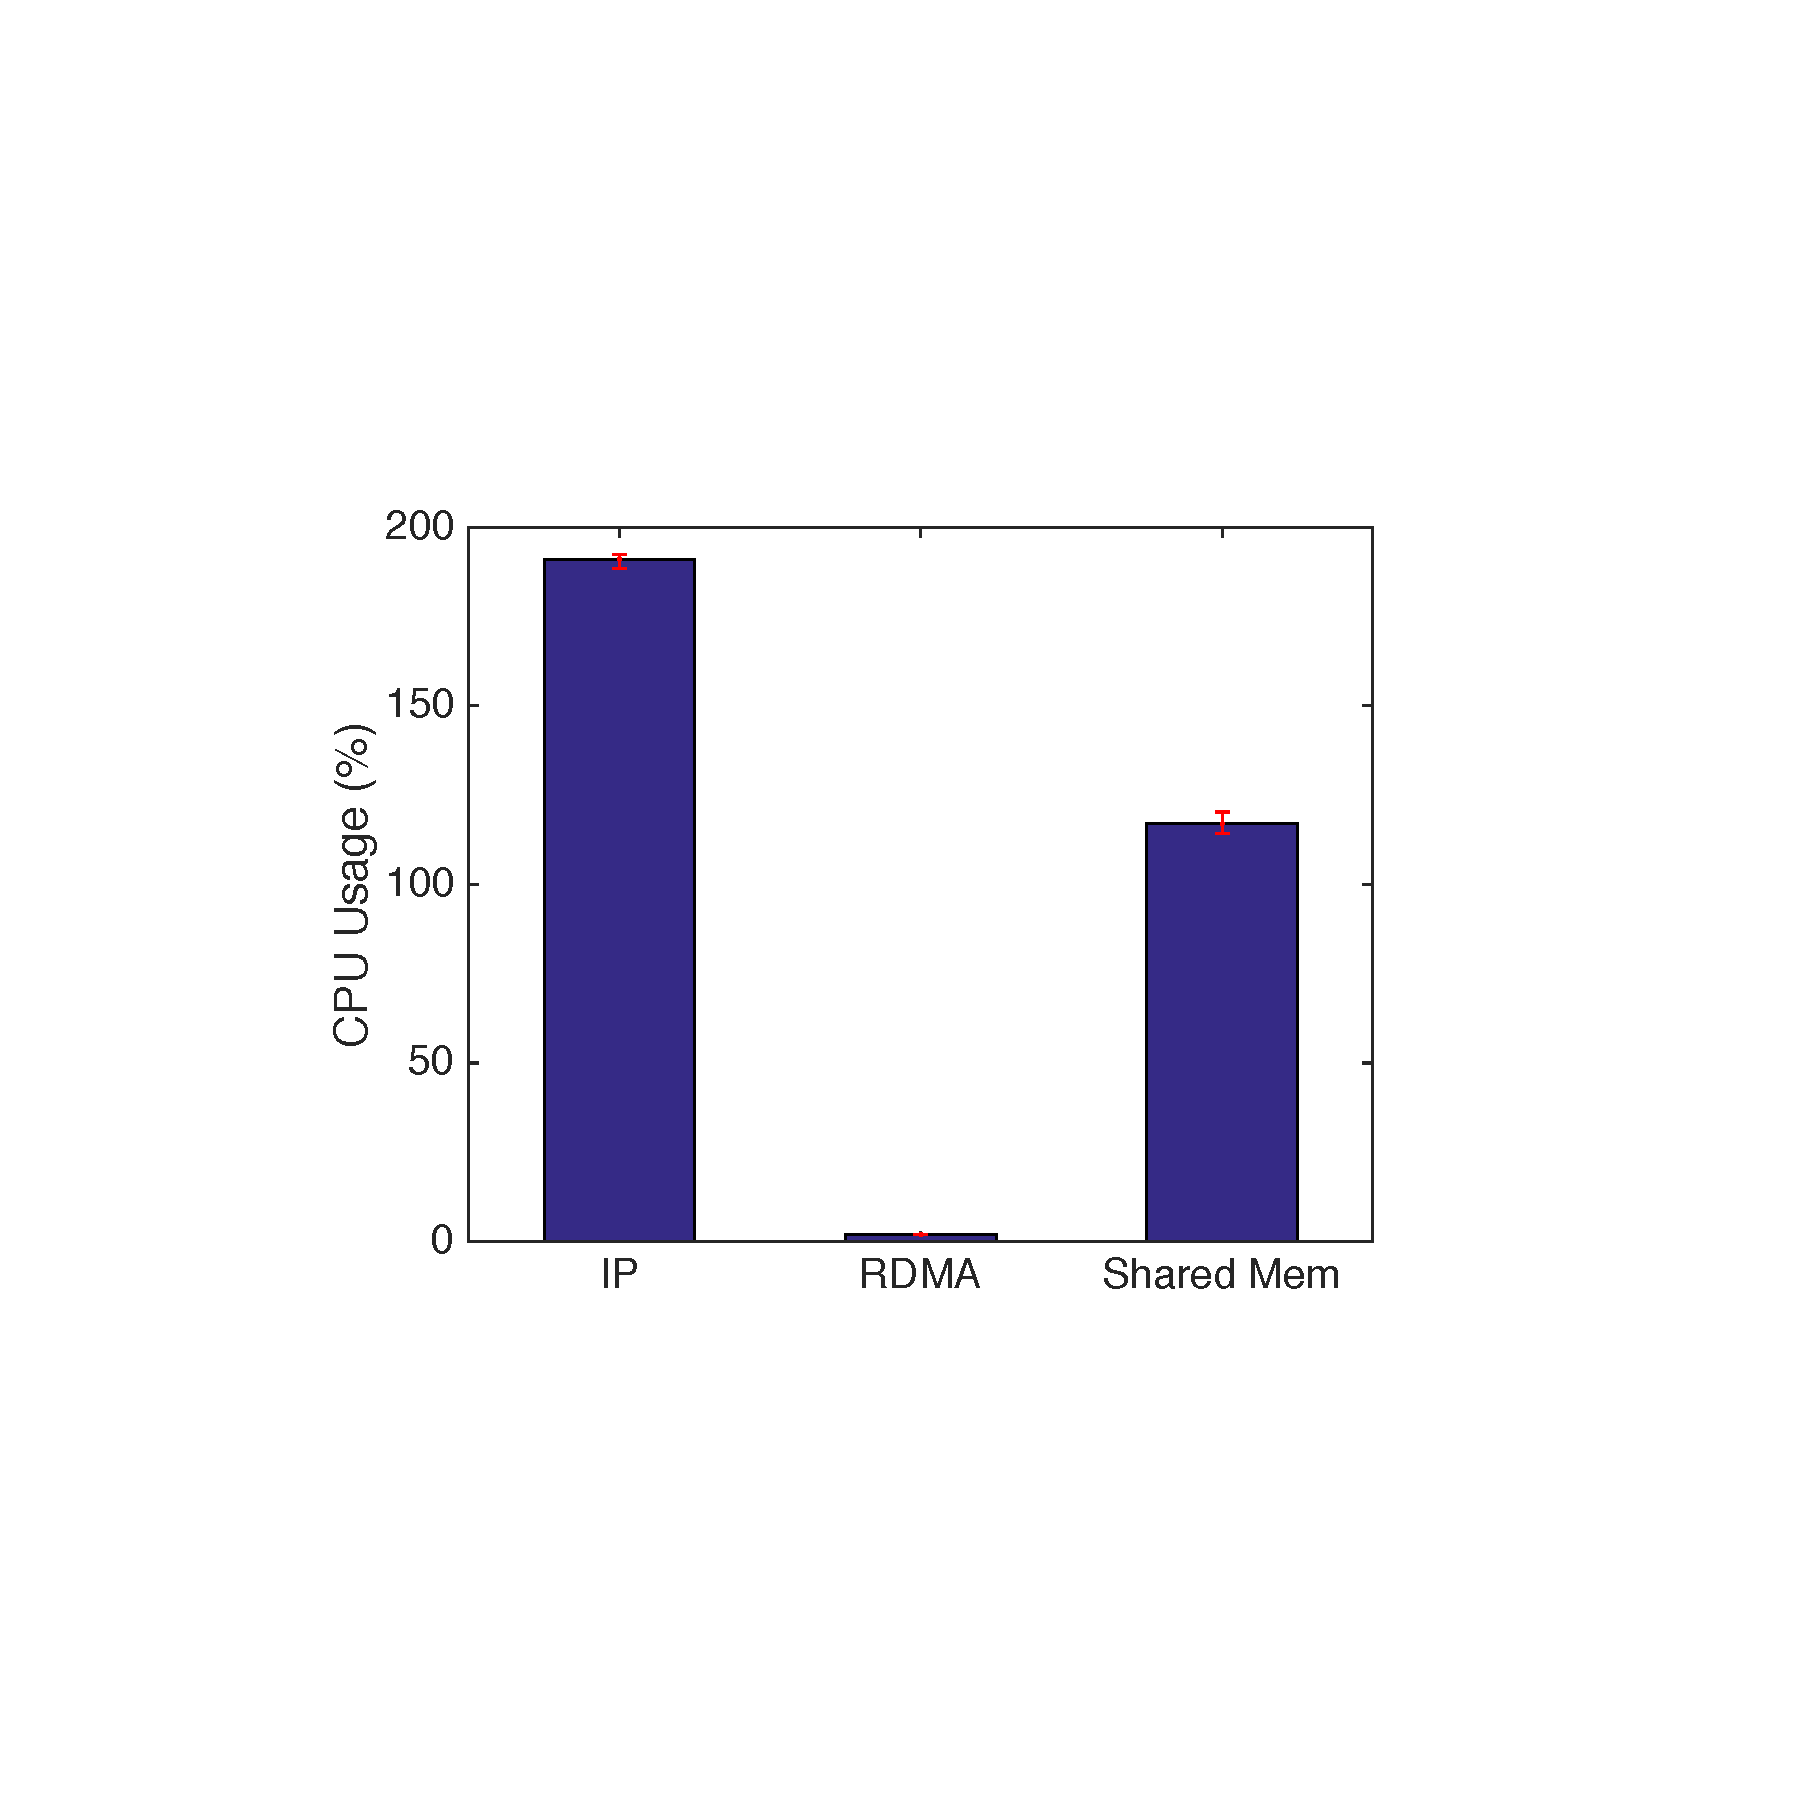
\includegraphics[width=0.32\textwidth]{figures/motivation/eval_baremetal_cpu.pdf}      
     %\label{fig:eval_baremetal_cpu}
     %\caption{} 
     \end{subfigure}           
     \label{fig:eval_baremetal_thr_latency_cpu}
     \caption{} 
\end{figure*} 

\begin{itemize}
  \item Communication via IP stack only achieves 27Gb/s throughput, 1 ms latency but uses near to 200\% of cpu.
  \item RDMA only improves the throughput to 40Gb/s for containers on the same machine, the latency is still 1ms, though it has a low cpu usage.
  \item Shared memory can achieve near-to-memory-bandwidth throughput, lowest latency, but still burns some cpu. 
\end{itemize}


\subsubsection{Host-mode vs. bridge mode}

\begin{figure}[!ht]
     \centering 
     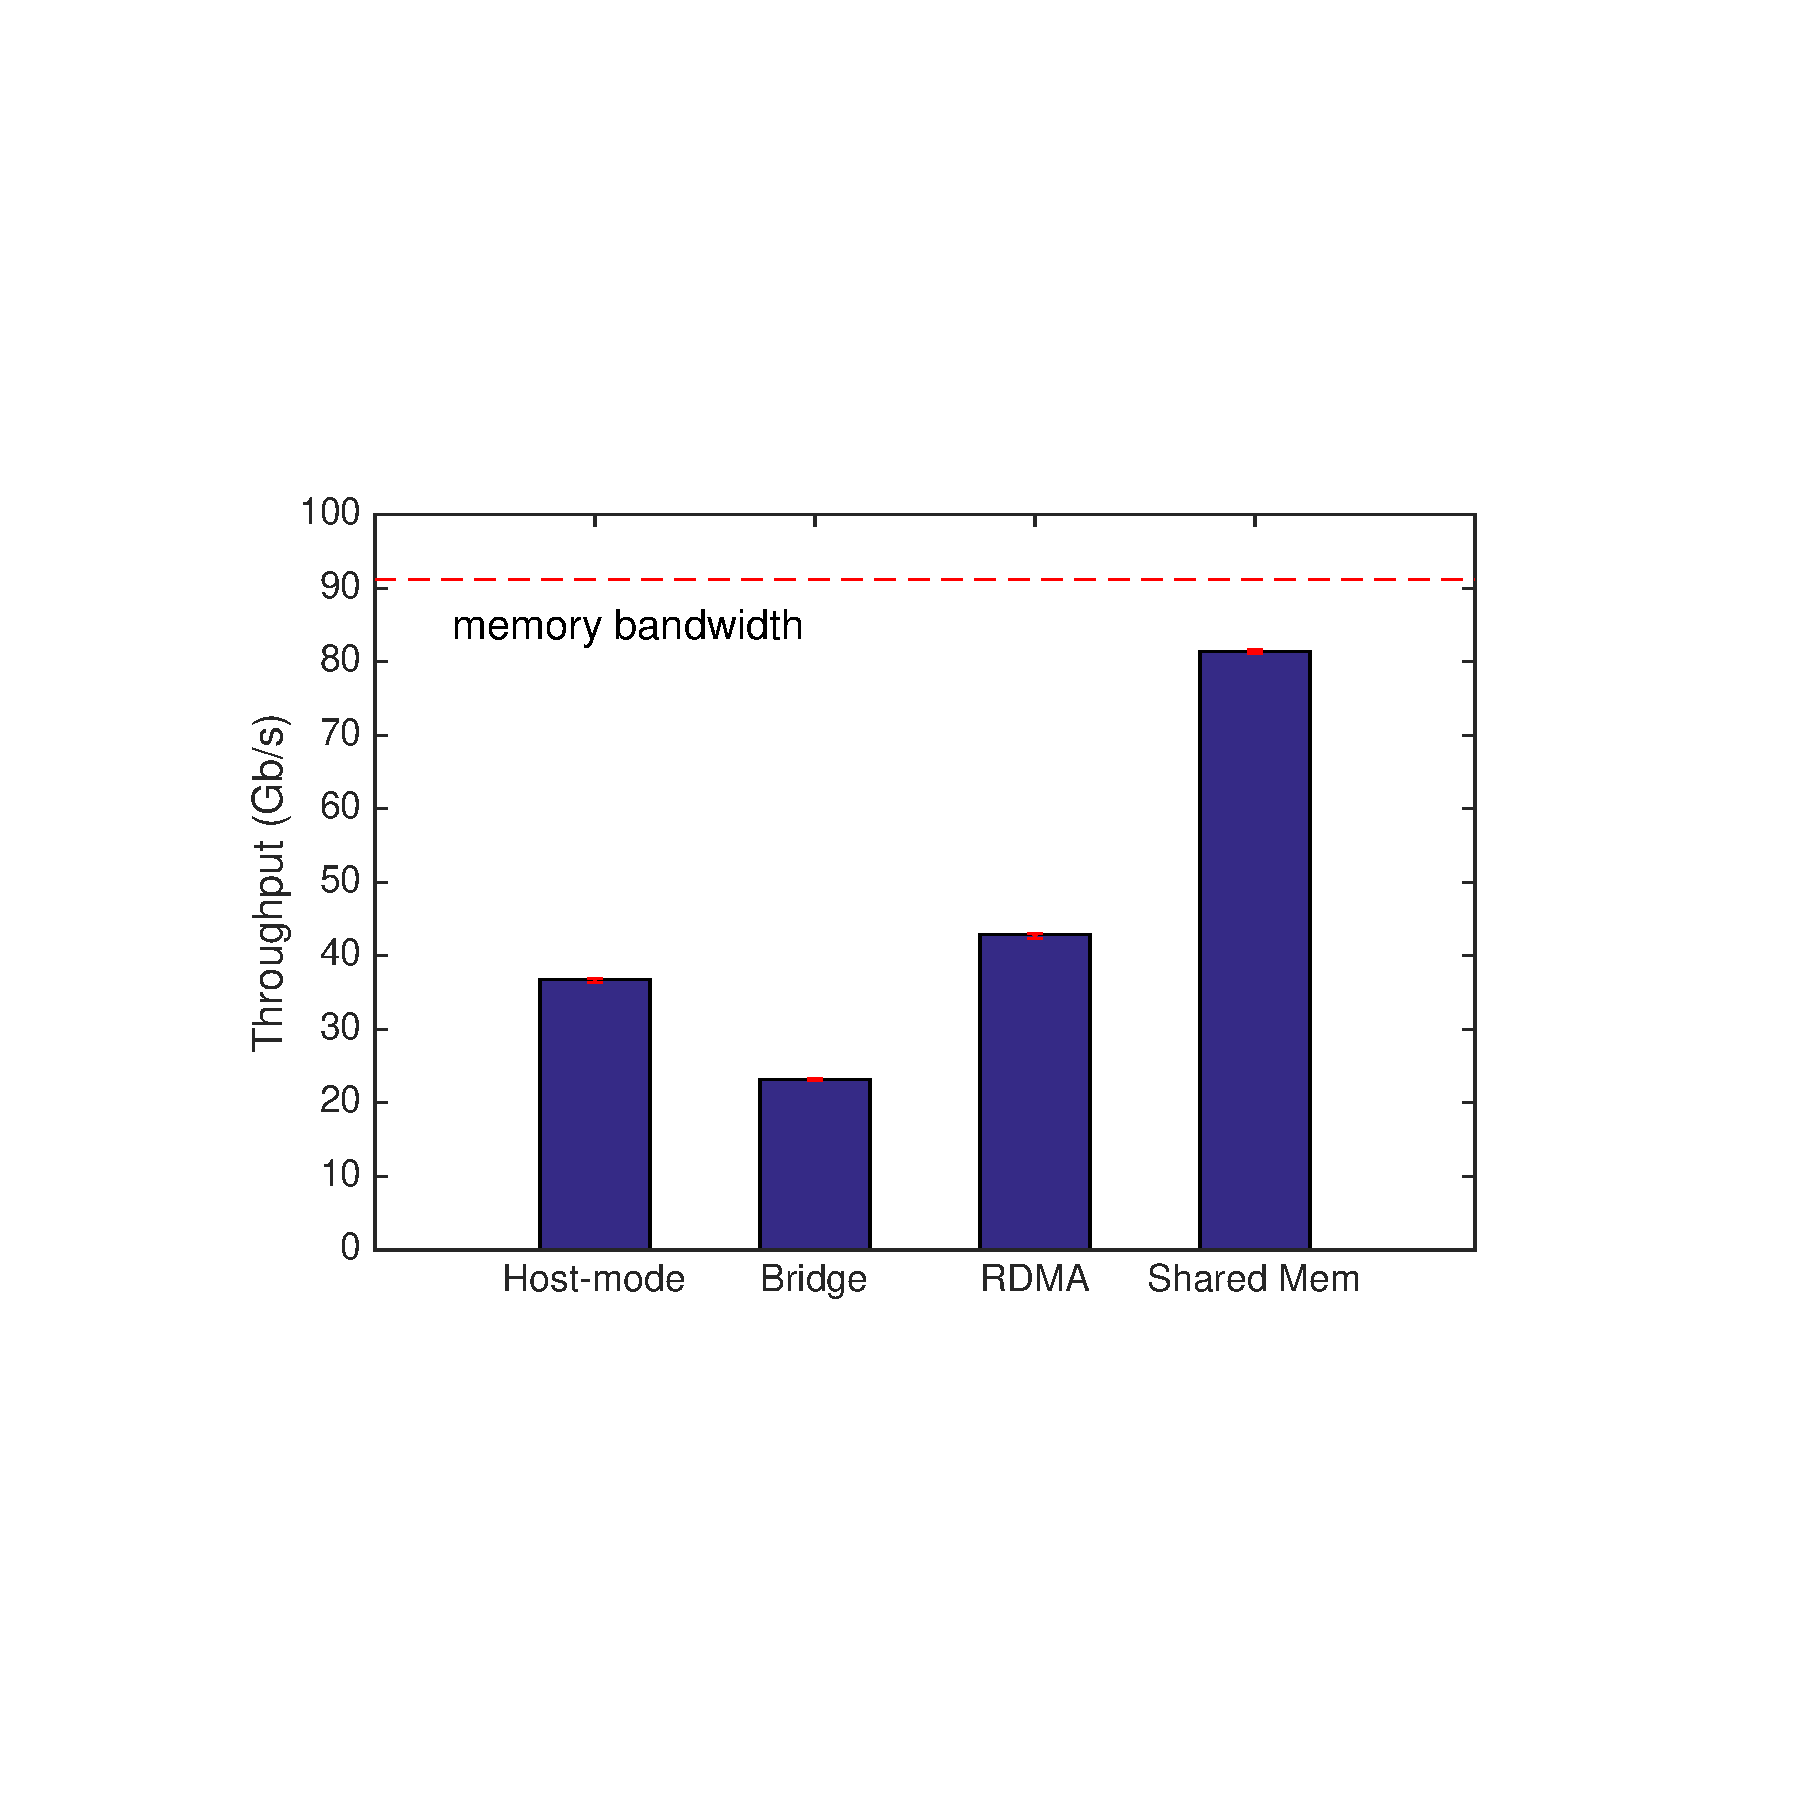
\includegraphics[width=3.35in]{figures/motivation/eval_bw_host_bridge.pdf} 
     \label{fig:eval_bw_host_bridge}
     \caption{ Host-mode vs. bridge mode vs. RDMA vs. shared memory.} 
\end{figure} 

\begin{itemize}
  \item Host-mode provides a better performance of 38 Gb/s. 
\end{itemize}

\subsection{Intra-host Network Performance}

\para{Throughput}

Three points: (1) TCP throughput is limited; (2) the bottleneck is CPU rather than memory bus for TCP/IP; (3) the bottleneck is NIC CPU for RDMA. (4) For intra-host cases, shared memory has the best performance.

Figure 1: throughput of single src-dst pair. Bar figure: x-axis: TCP/IP, RDMA and shared memory; y-axis: throughput;

Figure 2(a): throughput of multiple src-dst pair. Line figure: x-axis: number of pairs,; y-axis: throughput; Four lines: TCP/IP, RDMA, shared memory and memory bus.

Figure 2(b): CPU utilization. Line figure: x-axis: number of pairs,; y-axis: CPU utilization; Three lines: TCP/IP, RDMA, shared memory.

Figure 2(c): NIC CPU utilization. Line figure: x-axis: number of pairs,; y-axis: NIC CPU utilization; Three lines: TCP/IP, RDMA, shared memory.

\begin{figure}[!ht]
     \centering 
     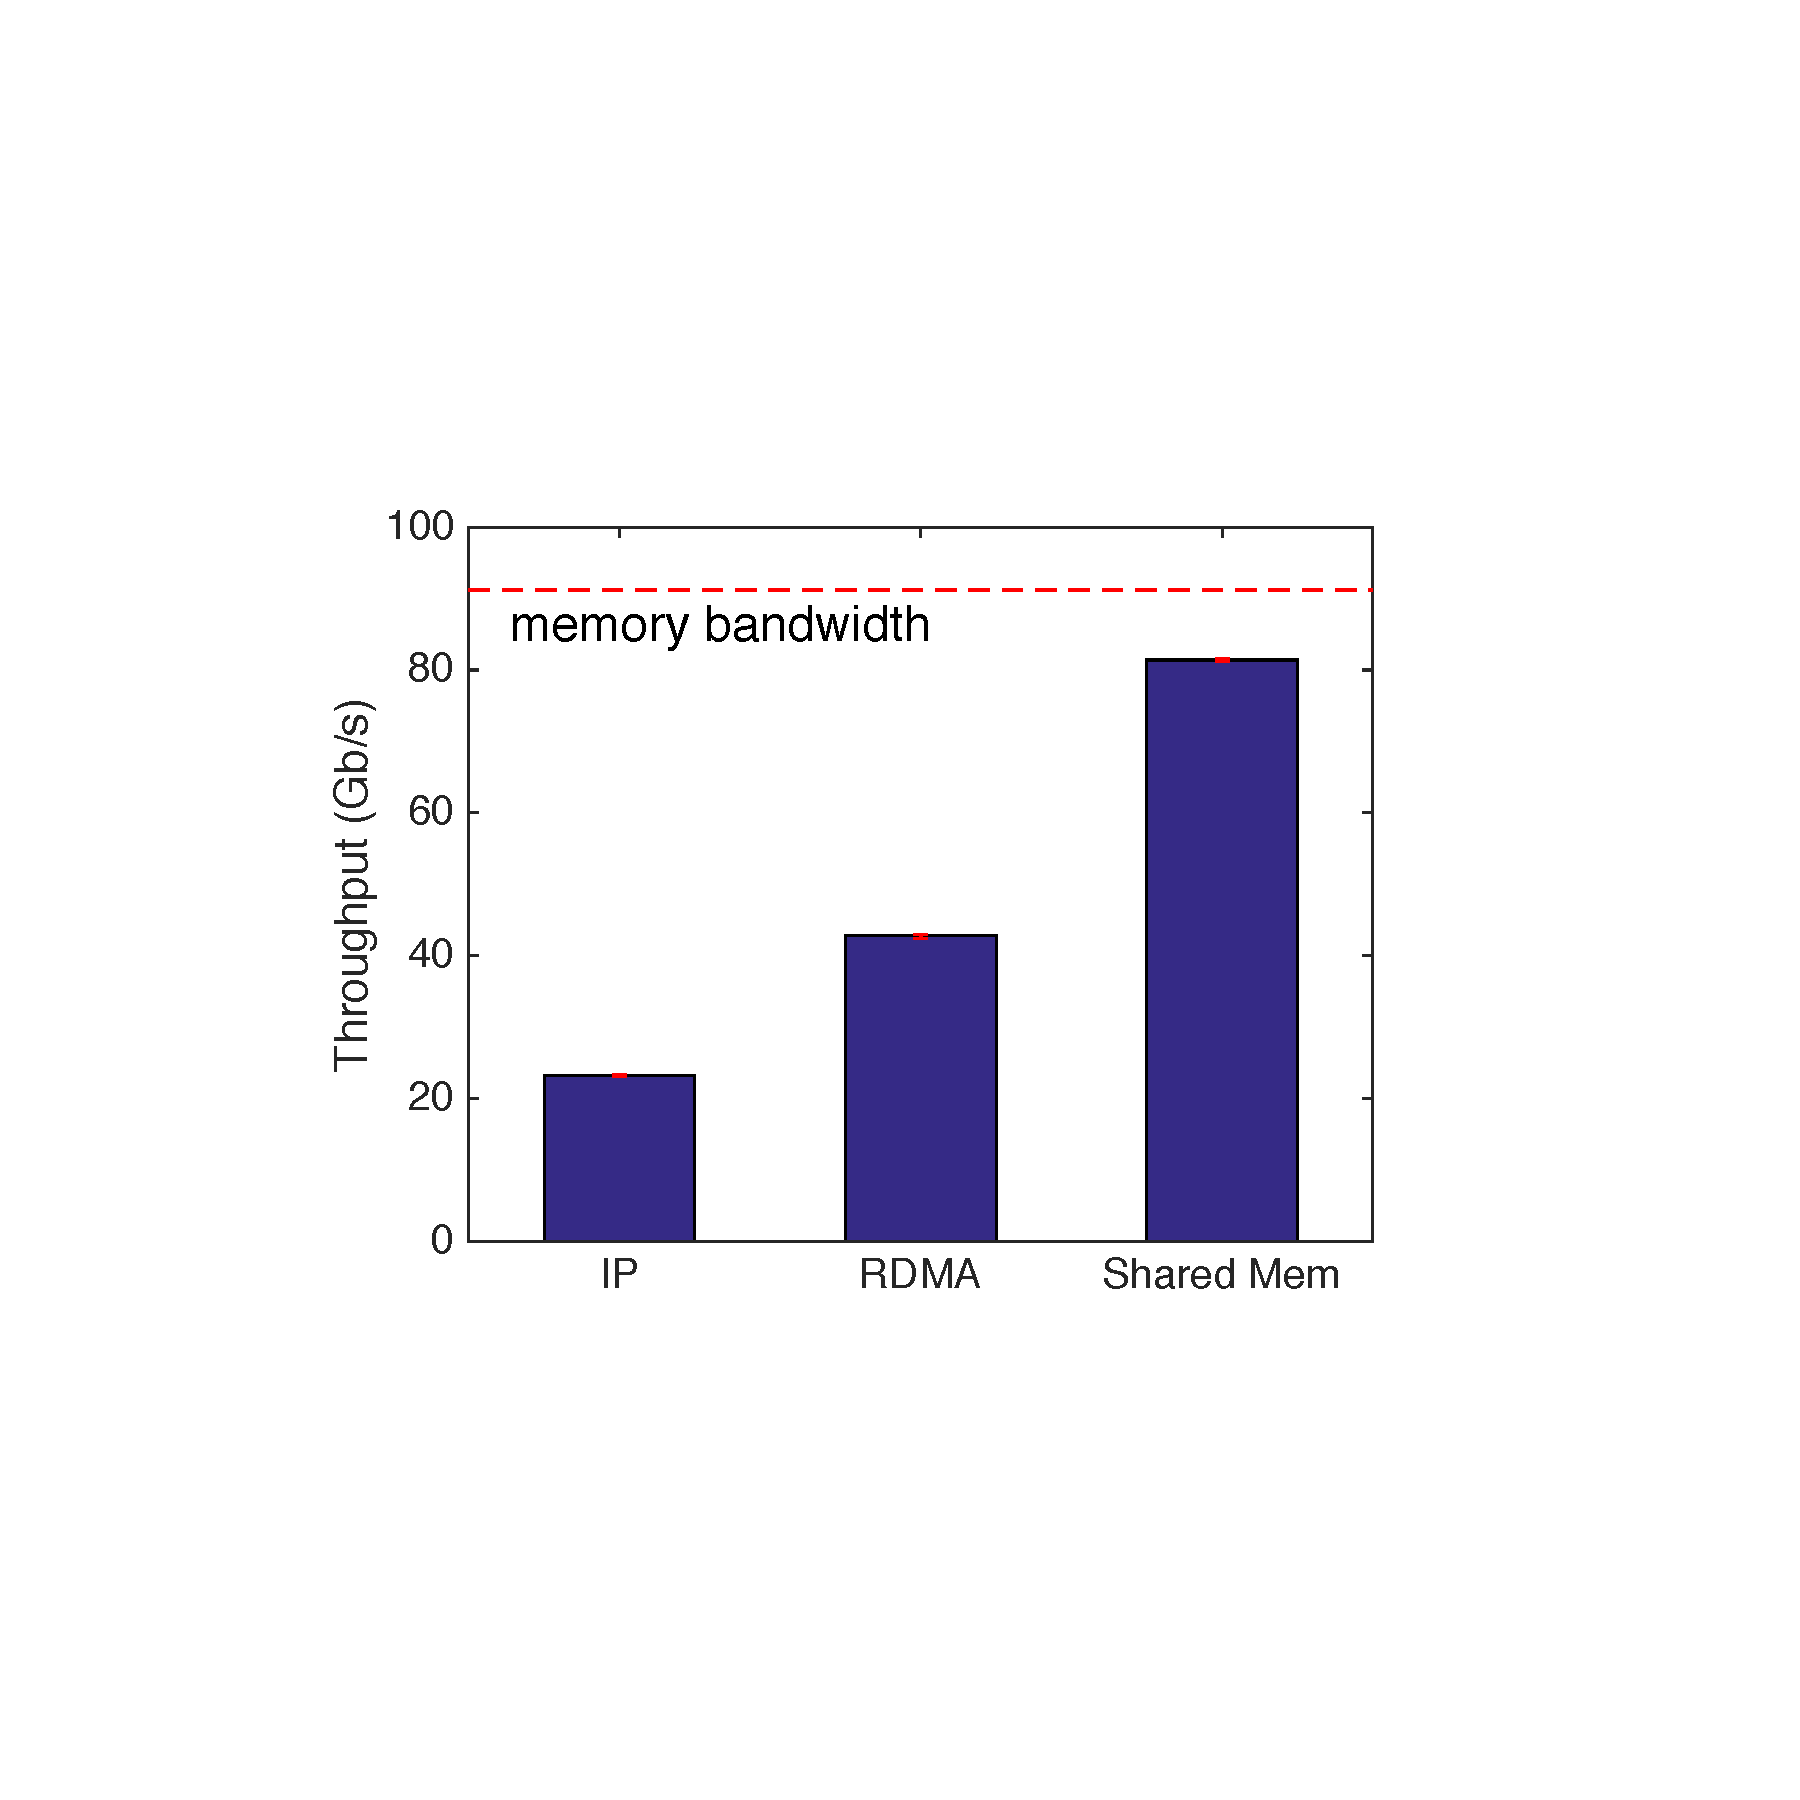
\includegraphics[width=3.35in]{figures/motivation/eval_baremetal_thr.pdf} 
     \caption{\label{fig:eval_baremetal_thr} The throughput of a pair of containers on the same bare metal communicating via IP stack, RDMA and shared memory. Communication via shared memory is close to the memory bandwidth.} 
\end{figure} 

\para{Latency}
Two points: (1) going through OS stack is increasing network latency; (2) The bottleneck is on system calls.

Figure 3: The stacked bar chart showing the total latency of TCP/IP, RDMA, shared memory and their components.

\begin{figure}[!ht]
     \centering 
     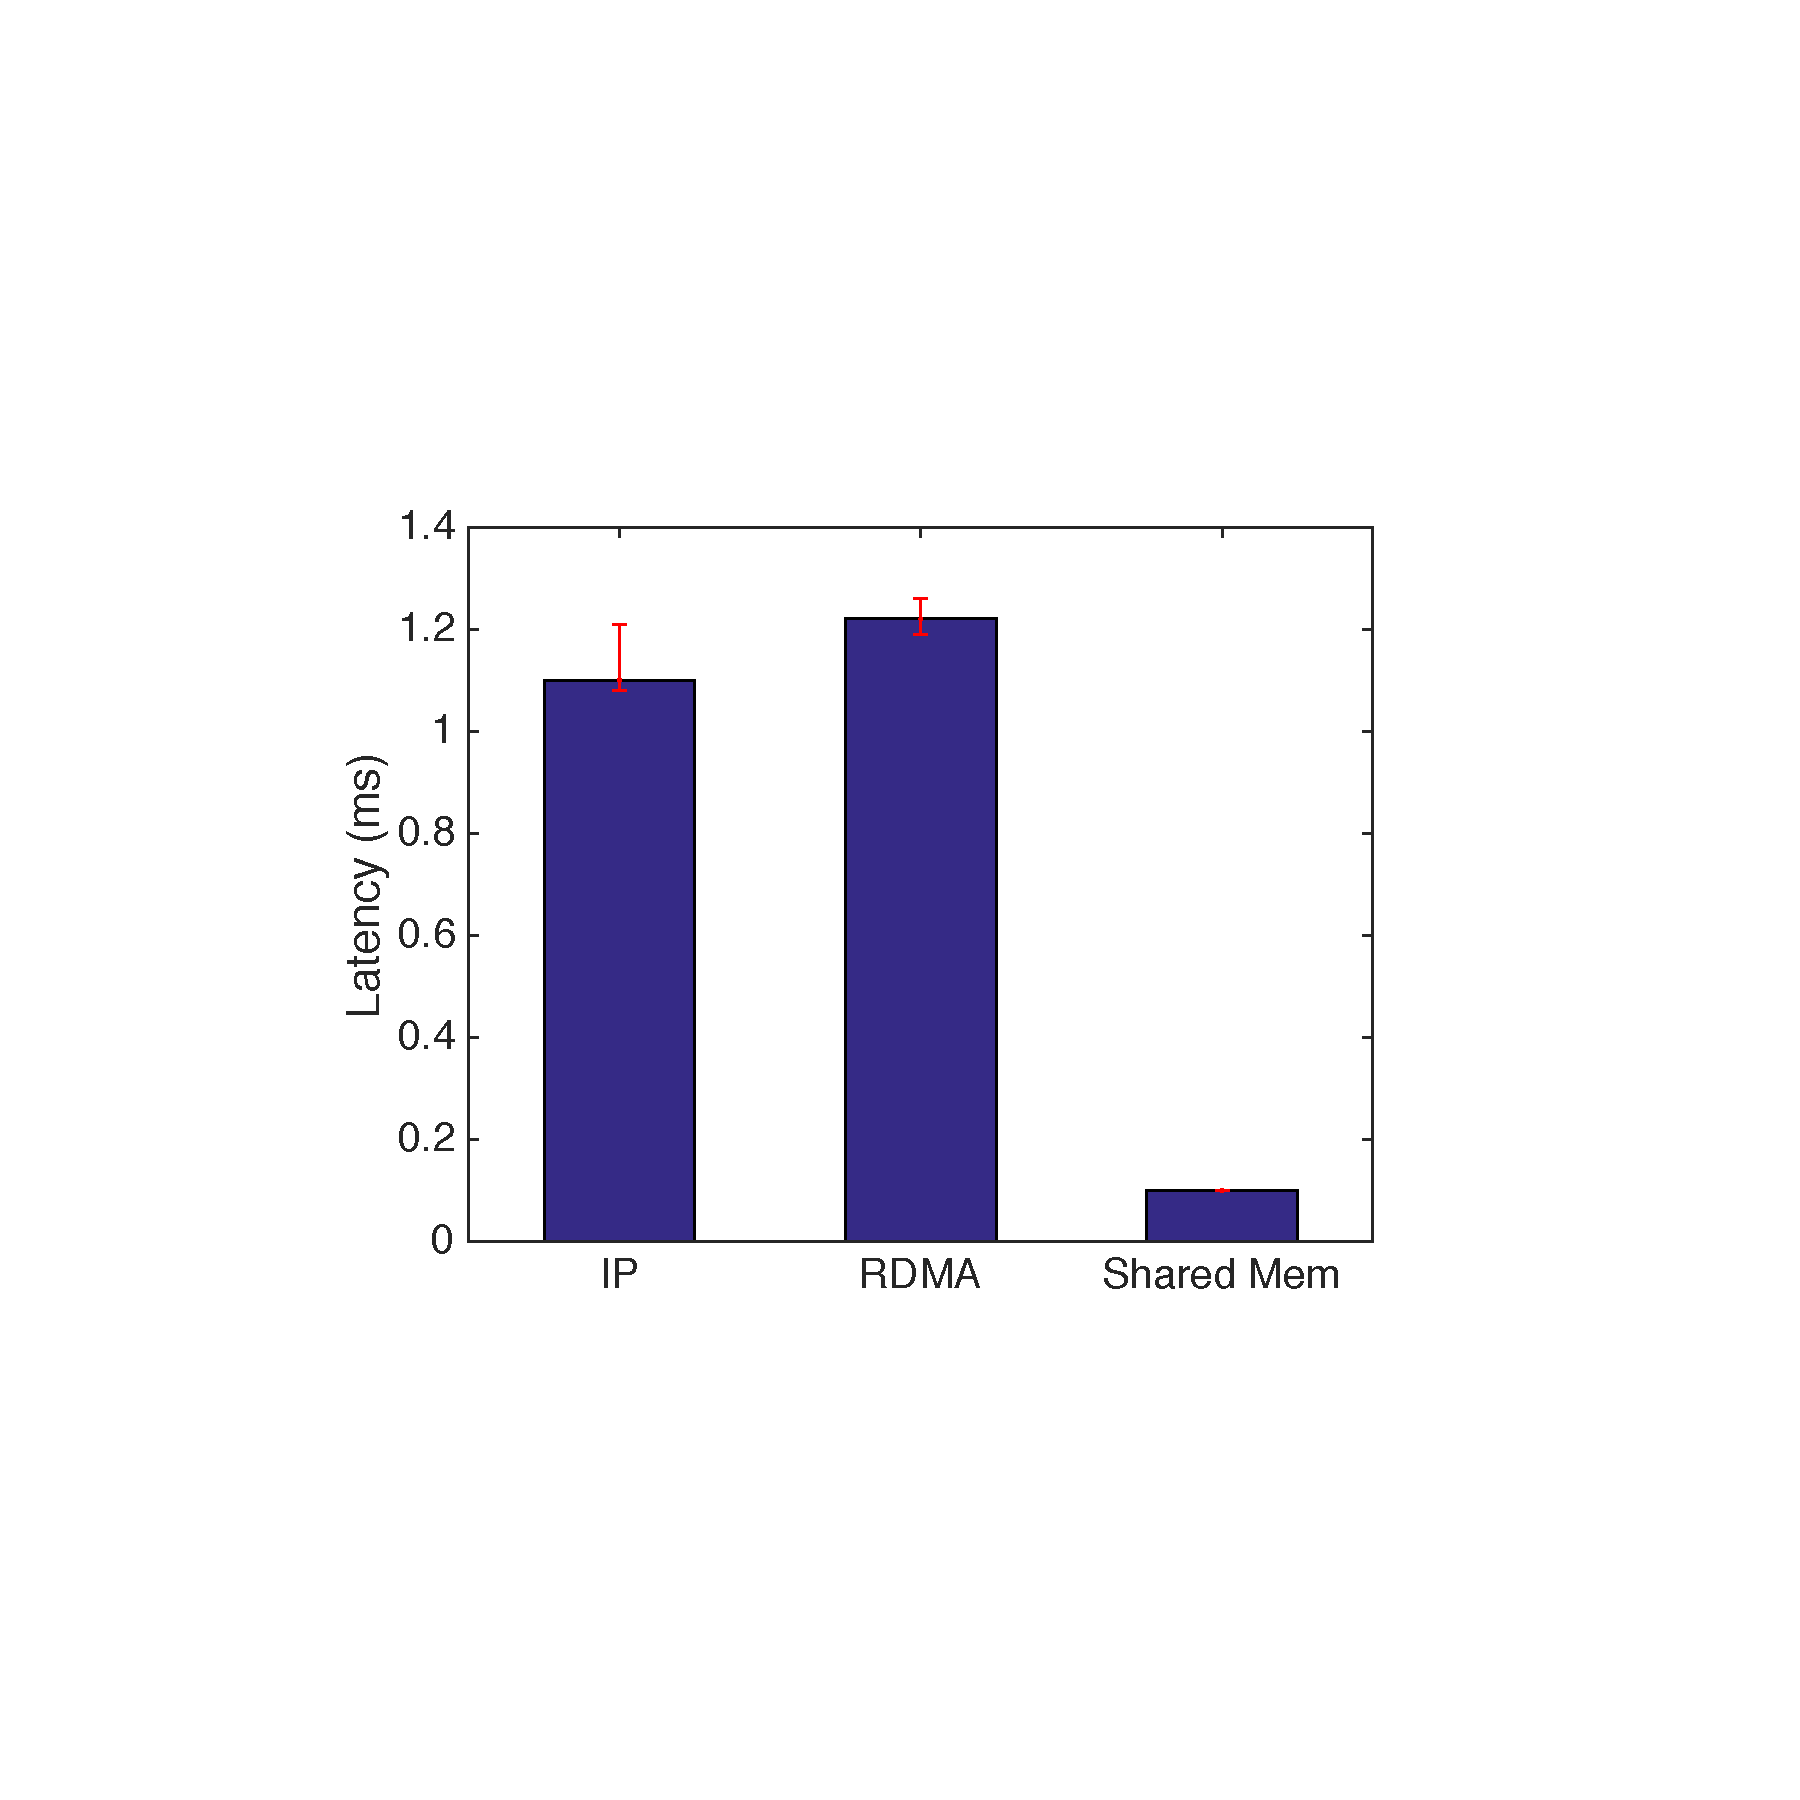
\includegraphics[width=3.35in]{figures/motivation/eval_baremetal_latency.pdf} 
     \caption{\label{fig:eval_baremetal_latency} The latency of a pair of containers on the same bare metal communicating via IP stack, RDMA and shared memory. Shared memory achieves the lowest latency.} 
\end{figure} 

\para{CPU Usage}

\begin{figure}[!ht]
     \centering 
     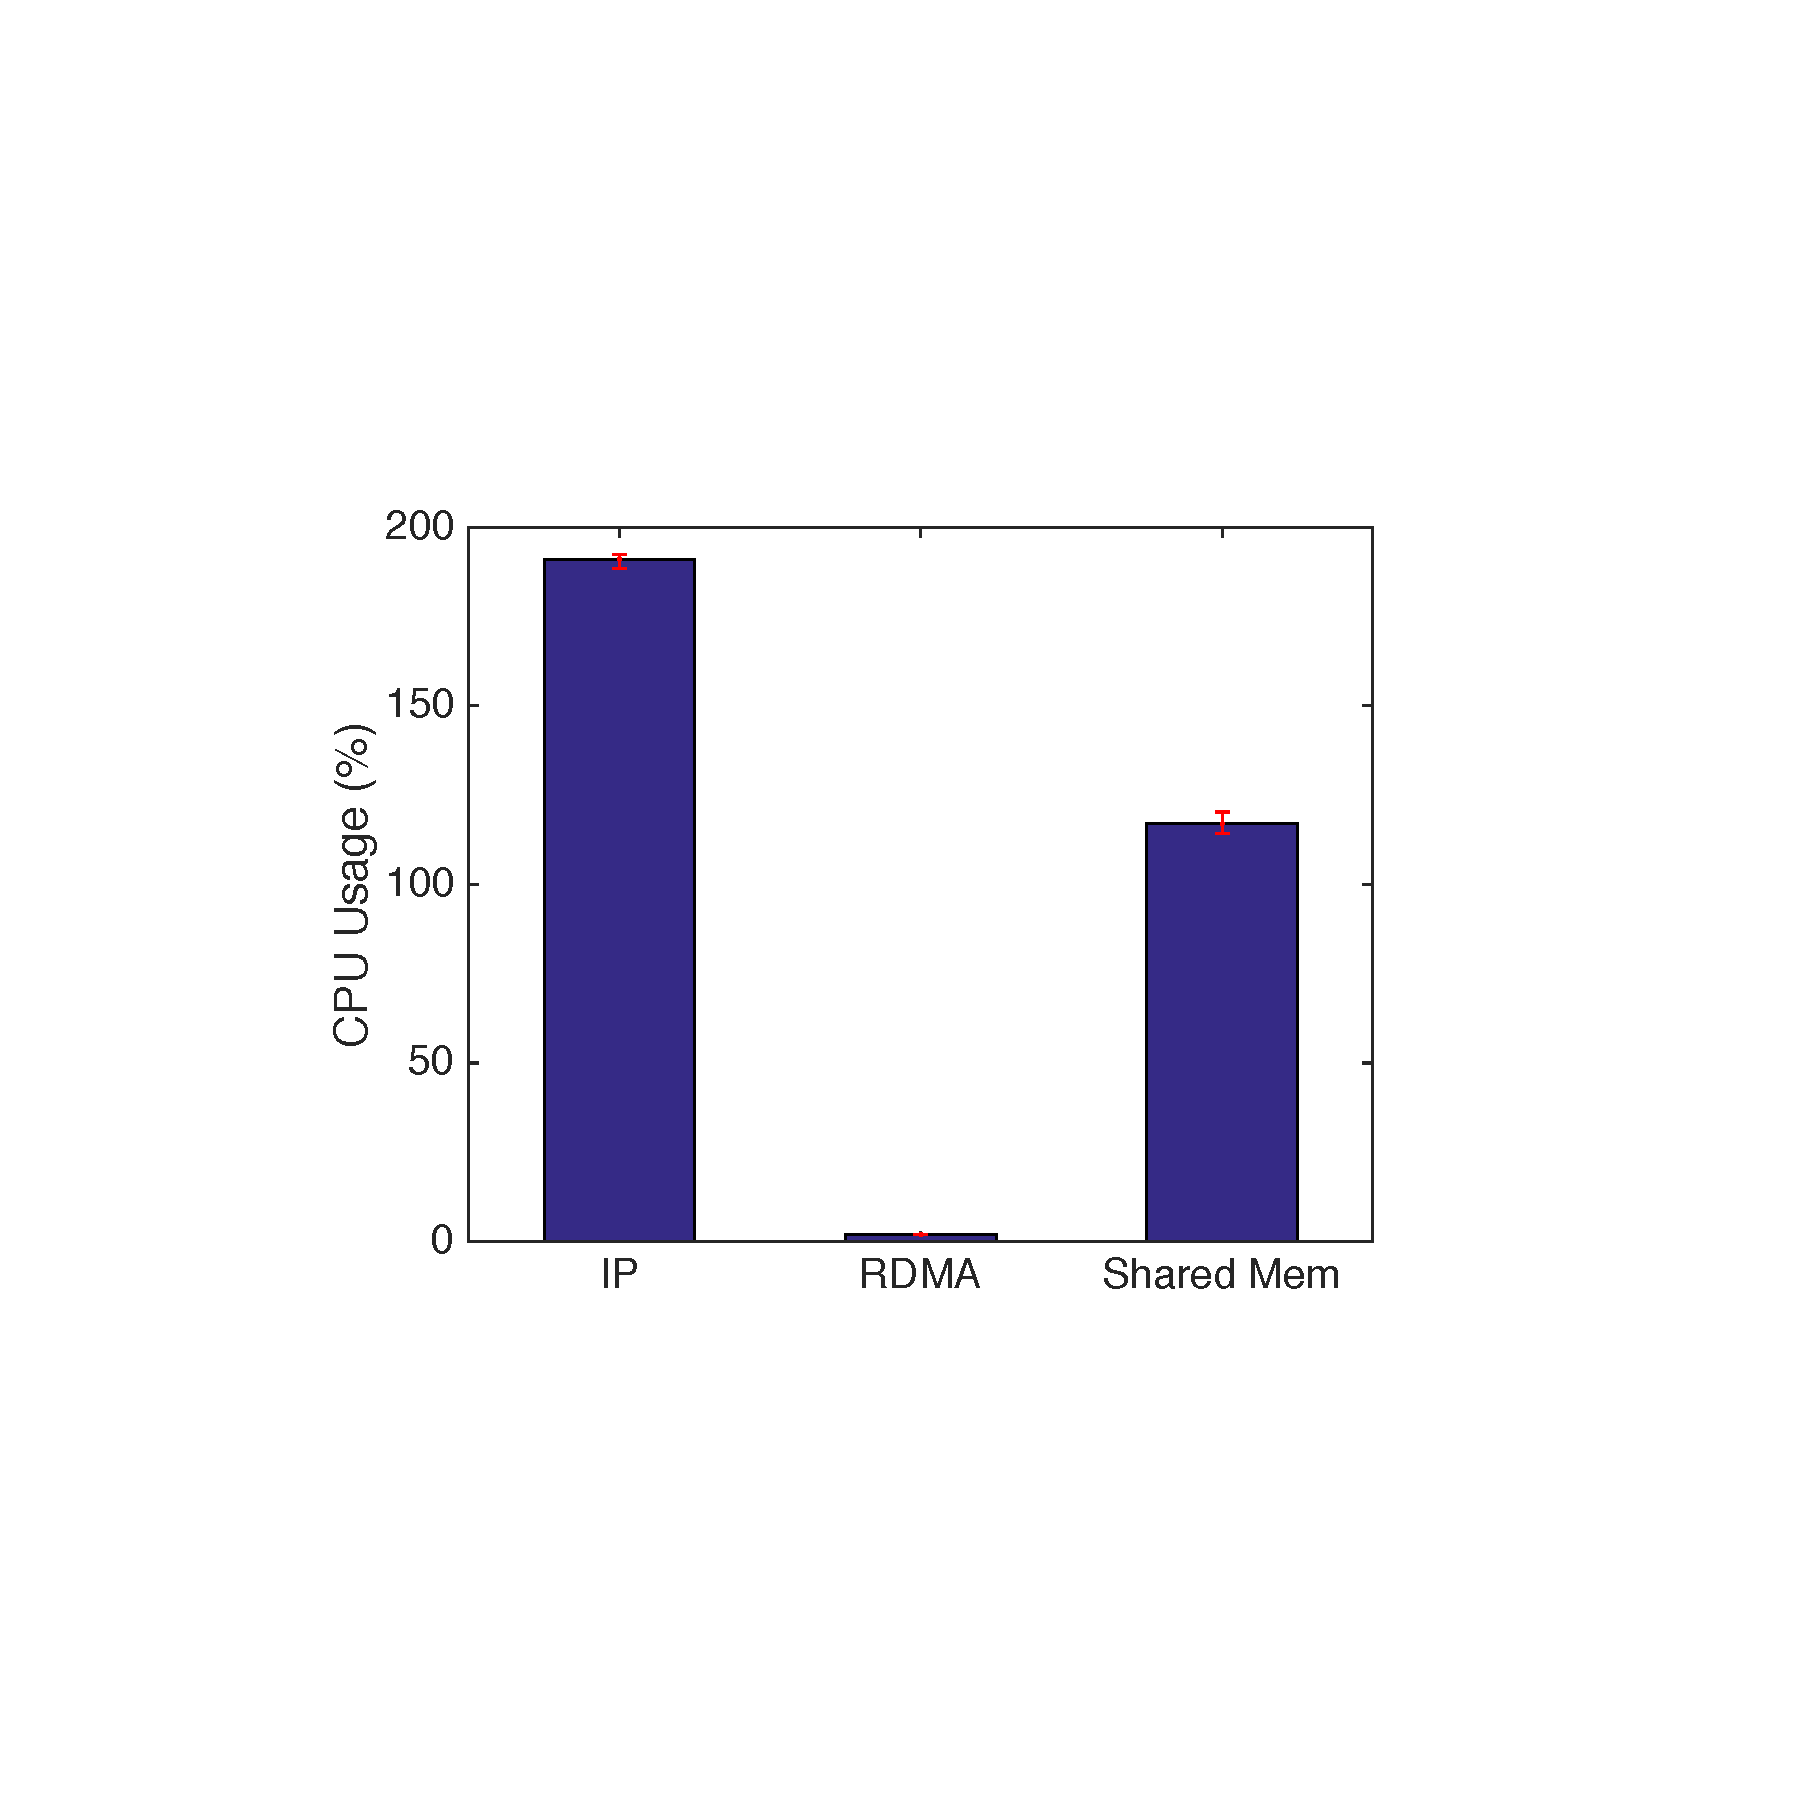
\includegraphics[width=3.35in]{figures/motivation/eval_baremetal_cpu.pdf} 
     \caption{\label{fig:eval_baremetal_cpu} The cpu usage of a pair of containers on the same bare metal communicating via IP stack, RDMA and shared memory. Communication via IP stack almost saturates 2 cpu cores.} 
\end{figure} 

% comment 
\fi
\section{Design} \label{sec:design}

\vyas{1. call this a overview section. 
2. move the insight nugget from previous section to here
3. before going to overview revisit the landscape of alternatives and kill them
4. main thing i want from this section is insight + sketch of what will change. this control/data is muddling that story IMO}

\begin{figure}[t!] 
     \centering 
     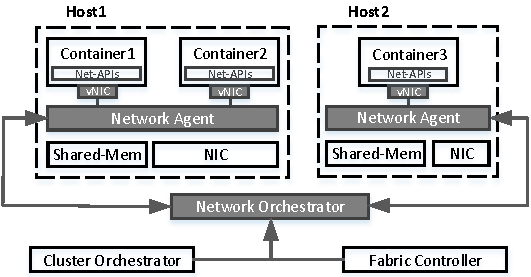
\includegraphics[width=3.2in]{figures/system-arch.pdf} 
    \caption{\label{fig:sysarch} The overall system architecture of~\sysname. Gray boxes are building blocks of~\sysname.} 
\end{figure} 

This section presents the high-level design of \sysname. We introduce
the requirements and concerns in the designs of control-plane, data-plane
and network access layer, and explain what design choices \sysname makes 
and what the reasons are behind these design choices.

\subsection{Overview}

Our goal is to design a complete network solution which can enable containers
to communicate with portability, isolation and high performance at the same time.
Basically, this solution has three major components: control-plane, data-plane 
and networking abstraction. 

\vyas{is this referring to ANY solution or OUR solution. im confused. also this ctr/data/abstraction is again 
a bit misleading .. its true for ANY network model, what is unique to container world here?}


A \textbf{control-plane} handles IP address assignment, routing and manages global states of a container network.
A flexible control-plane is a must for portability and isolation. 
It should permit a container to register its own IP address in the network
from any host; It also should automatically configure and update the routing 
to each container. One unique requirement for \sysname's control-plane,
compared with existing container networking solutions, is to be able to 
select data-plane (e.g. shared-memory, RDMA, TCP/IP, etc.) in real-time
according to multiple factors, such as container locations, hardware 
capabilities and so on. 
There are several routing schemes that are used by existing
container networking solutions, and they are optional for \sysname. 
For example, Calico and WeaveNet build distributed routing scheme on top of 
distributed routing protocols (e.g. BGP), while Docker default overlay network
and DaoliNet use centralized routing planes based on OpenFlow and OVS.

A \textbf{data-plane} delivers data from sender containers to receiver 
containers. \sysname's data-plane should always achieve a good trade-off
between isolation, portability and performance. 
As introduced in \S\ref{sec:motivation}, there are many data-plane mechanisms
for two containers, such as shared-memory (intro-host), TCP/IP, DPDK, RDMA, etc..
Different mechanisms have different properties on portability, isolation and 
performance. Therefore, we need to decide is to choose a single mechanism, or
integrate multiple mechanisms together.

A \textbf{network abstraction} defines how containers access the networks
provided by \sysname. Application inside containers are using existing 
network APIs, e.g. Socket for TCP/IP, Verbs for RDMA, MPI for parallel computing, etc., so \sysname must support all of them seamlessly for 
backward compatibility. On the other hand, the actual data-plane mechanism
should be hidden behind the network abstraction layer and transparent to 
application code. There are two options to realize a network abstraction.
The first option is to modify the implementation all libraries of existing
network APIs. When applications calls the APIs, \sysname intercepts
the function calls and performance its logic of networking. 
The second option is to let \sysname only support one API semantics for
data transfers, and develop translation layer which convert different
existing API semantics into the one supported by \sysname.

The design of~\sysname fully considers the requirements from all these three
components.

\subsection{Design choices of FreeFlow}

Figure~\ref{fig:sysarch} shows the architecture and design choices on each 
components of~\sysname. Network orchestrator and the network agents compose 
the centralized control-plane of~\sysname. The network agent running in each 
host coordinates multiple data-plane mechanisms according to the information and 
configurations feed from the network orchestrator. RDMA Verbs is selected as 
the basic interface for data transfers in the network abstraction. \vyas{please nuke/reword the previous section. dont make the RDMA the CRUX of the solution. its a recipe
 for disaster.} Different networking APIs (e.g. Socket) for data
transfers are translated to the semantics of RDMA and performed by the RDMA
Verbs library. A virtual RDMA NIC is created for each container to make the
actual data-plane mechanism transparent to Verbs library.

\para{Centralized control-plane:} \sysname inherently needs a (conceptually)
centralized control-plane because the IP assignment, routing configuration and 
data-plane mechanism decisions are all computed from the global states of the
container cluster. The network orchestrator of~\sysname maintains three kinds
of global information: the location of each container (from cluster orchestrator), the assigned IP of each
container and the capabilities of host NICs. If containers are running on top of
VMs, the network orchestrator also needs to know which physical machine each VM 
is located (from fabric controllers). Container IPs can be assigned 
automatically by network agents via DHCP, or manually assigned by containers' 
configurations. The traffic from a sender
to a receiver is routed by the sender's network agent directly to 
the receiver's network agent, assuming the connectivity between
any pair of host is always maintained by the host network. 

\para{Integrated Data-plane:} \sysname integrates multiple data-plane 
mechanisms. The network agent on each host 
obtains the container location information from the network orchestrator. 
It decides to use shared-memory to communicate if two containers are on the
same host, otherwise, it will conduct the communicate going through 
the NIC of its host. Depending on the capability of the NIC, the traffic 
between two hosts can be delivered via RDMA, DPDK or TCP/IP.

\para{Network abstraction with virtual NICs:} 
We choose to provide a single data transfer API which is RDMA Verbs for two
reasons. First of all, RDMA Verbs is flexible for upper-layer APIs.
RDMA Verbs is a general message-passing API which can 
easily support multiple API semantics on its top. There are already libraries
available to translate TCP/IP~\cite{?} and MPI APIs~\cite{?} to RDMA Verbs 
semantics. 
Second, RDMA Verbs is also flexible to under-layer data-plane mechanism. 
The actual data-plane of RDMA Verbs can be either RDMA enabled networks and 
ordinary IP networks (using TCP as a transport). 
In addition, its memory copying APIs can 
easily support shared-memory semantics on the data-plane. 

In next section, we will discussion about our implementation plan of \sysname.

\vyas{here is my problem with this section. at the end of the day i dont get a AHA insight from this section nor can i really 
 envision  how the world will change because of your insight and what the steps to that will be. in some sense this sounds more 
like the detailed design in sec 4 rather than the arch overview for sec 3. i really dont like fig 4 --> i cant quickly understand 
 what YOUR insight/prposal is. it looks like the same as every other figure you have drawn so far}

%\subsection{Working flows of FreeFlow}

%To support the standard RDMA Verbs API used by containers and realize
%communications with the best available data-plane mechanism, \sysname needs
%to present a RDMA environment to containers and efficiently supports 
%the RDMA semantics with multiple data-plane mechanisms. While RDMA has
%four interfaces (e.g. Write, Read, Send and Receive), we use Write as an example
%to show how \sysname supports this operation with shared-memory and real RDMA.

%Figure XXX (a) shows the working flow of a standard RDMA write from containers'
%points of view when they use Verbs API. There are generally three steps in a 
%Write operation. 
%Step 1: the sender first creates a memory block, puts data in it and passes 
%the pointer of this memory block to its NIC;
%Step 2: the sender notify its NIC to write the memory block to the receiver's IP.
%Step 3: the receiver's NIC will get data from the sender's NIC and copy the 
%data into a memory block and pass the pointer of the memory block to the 
%receiver.

%In \sysname, both the sender and receiver containers have a virtual RDMA NIC.
%In Step 1, the sender creates a shared-memory block and write data, and then 
%the local network agent will get the pointer of this shared-memory block after %the sender passes it to its virtual NIC; In Step 2, after receiving the IP of 
%the receiver, the local network agent will check whether the receiver is on
%the same host of the sender. If the answer is "Yes", the local network agent %will
%directly leverage the receiver's virtual NIC to notify it that a memory block 
%from RDMA is ready to read with the pointer of the shared-memory block. 
%Otherwise, the sender's local network agent will perform an actual RDMA write
%with the receiver's local network agent, and the latter will put the received data into a shared-memory and pass it to the receiver container via its virtual NIC.







\section{System to Build} \label{sec:promise}

To support the standard RDMA Verbs API used by containers and realize
communications with the best available data-plane mechanism, \sysname needs
to present a RDMA environment to containers and efficiently supports 
the RDMA semantics with multiple data-plane mechanisms. While RDMA has
four interfaces (e.g. Write, Read, Send and Receive), we use Write as an example
to show how \sysname supports this operation with shared-memory and real RDMA.

     \begin{figure}[ht]
     \centering 
     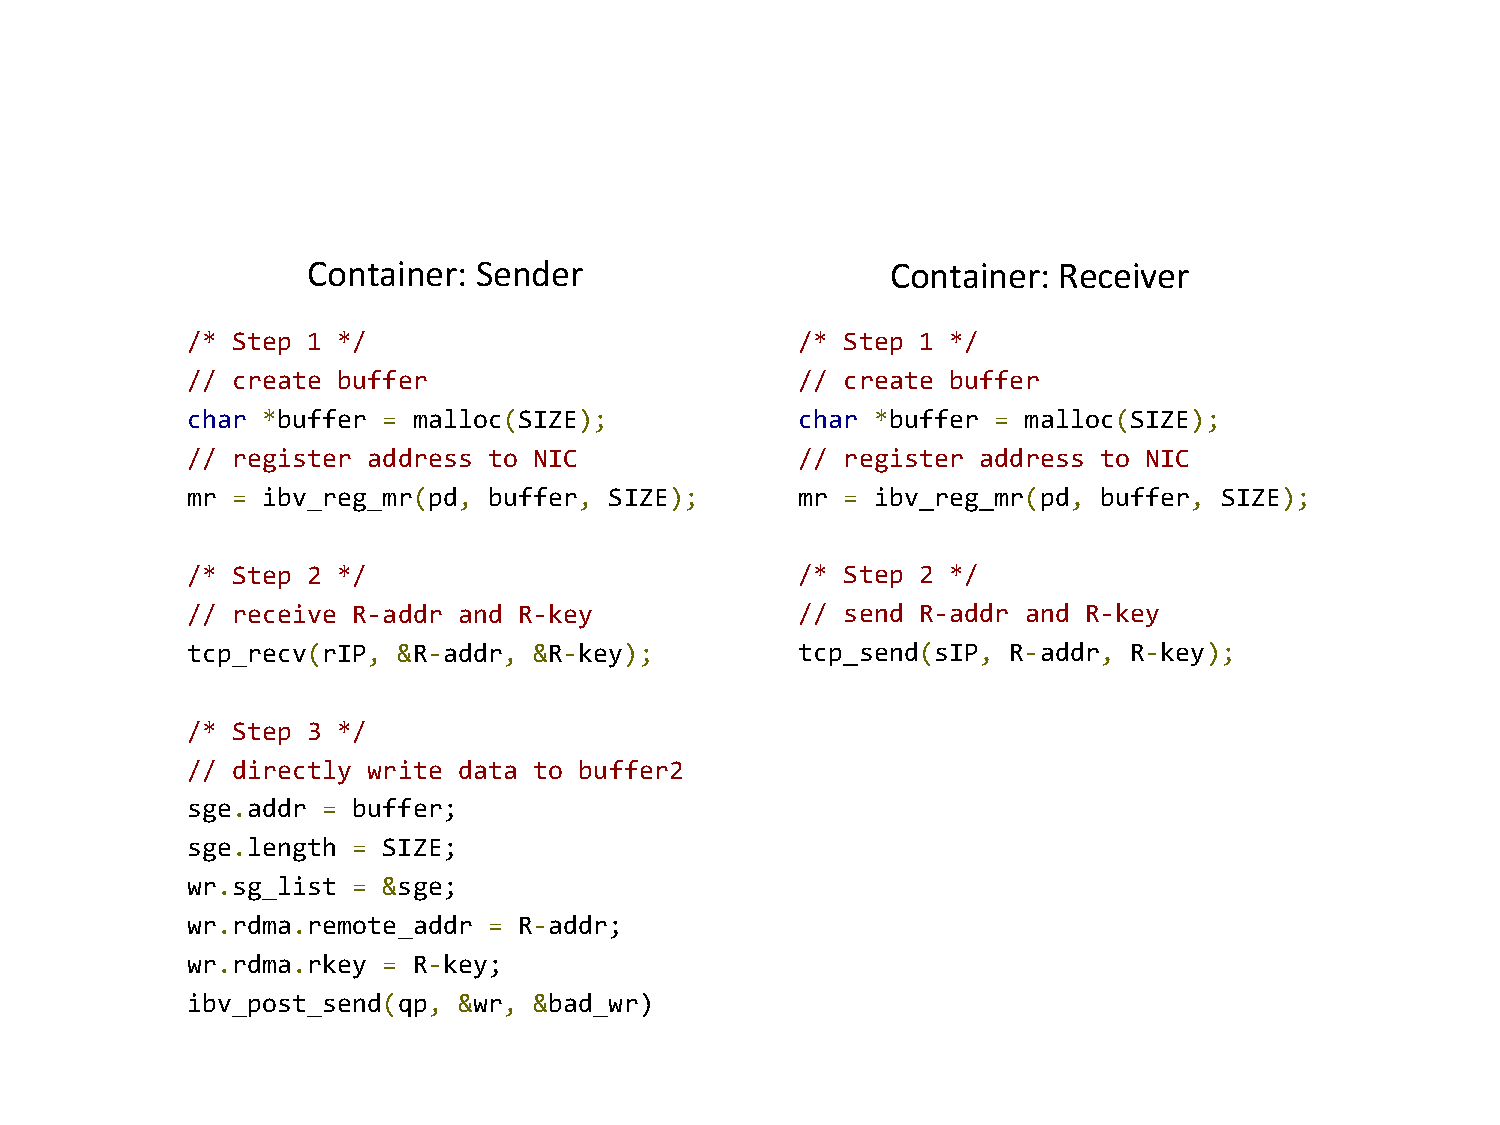
\includegraphics[width=0.45\textwidth]{figures/system/sys_rdma_code.pdf}      
     \label{fig:sys_rdma_code}
     \caption{The psudo code of an application execute RDMA write.} 
     \end{figure}

Figure XXX (a) shows the working flow of a standard RDMA write from containers'
points of view when they use Verbs API. There are generally three steps in a 
Write operation. 
Step 1: the sender first creates a memory block, puts data in it and passes 
the pointer of this memory block to its NIC;
Step 2: the sender notify its NIC to write the memory block to the receiver's IP.
Step 3: the receiver's NIC will get data from the sender's NIC and copy the 
data into a memory block and pass the pointer of the memory block to the 
receiver.

     \begin{figure}[ht]
     \centering 
     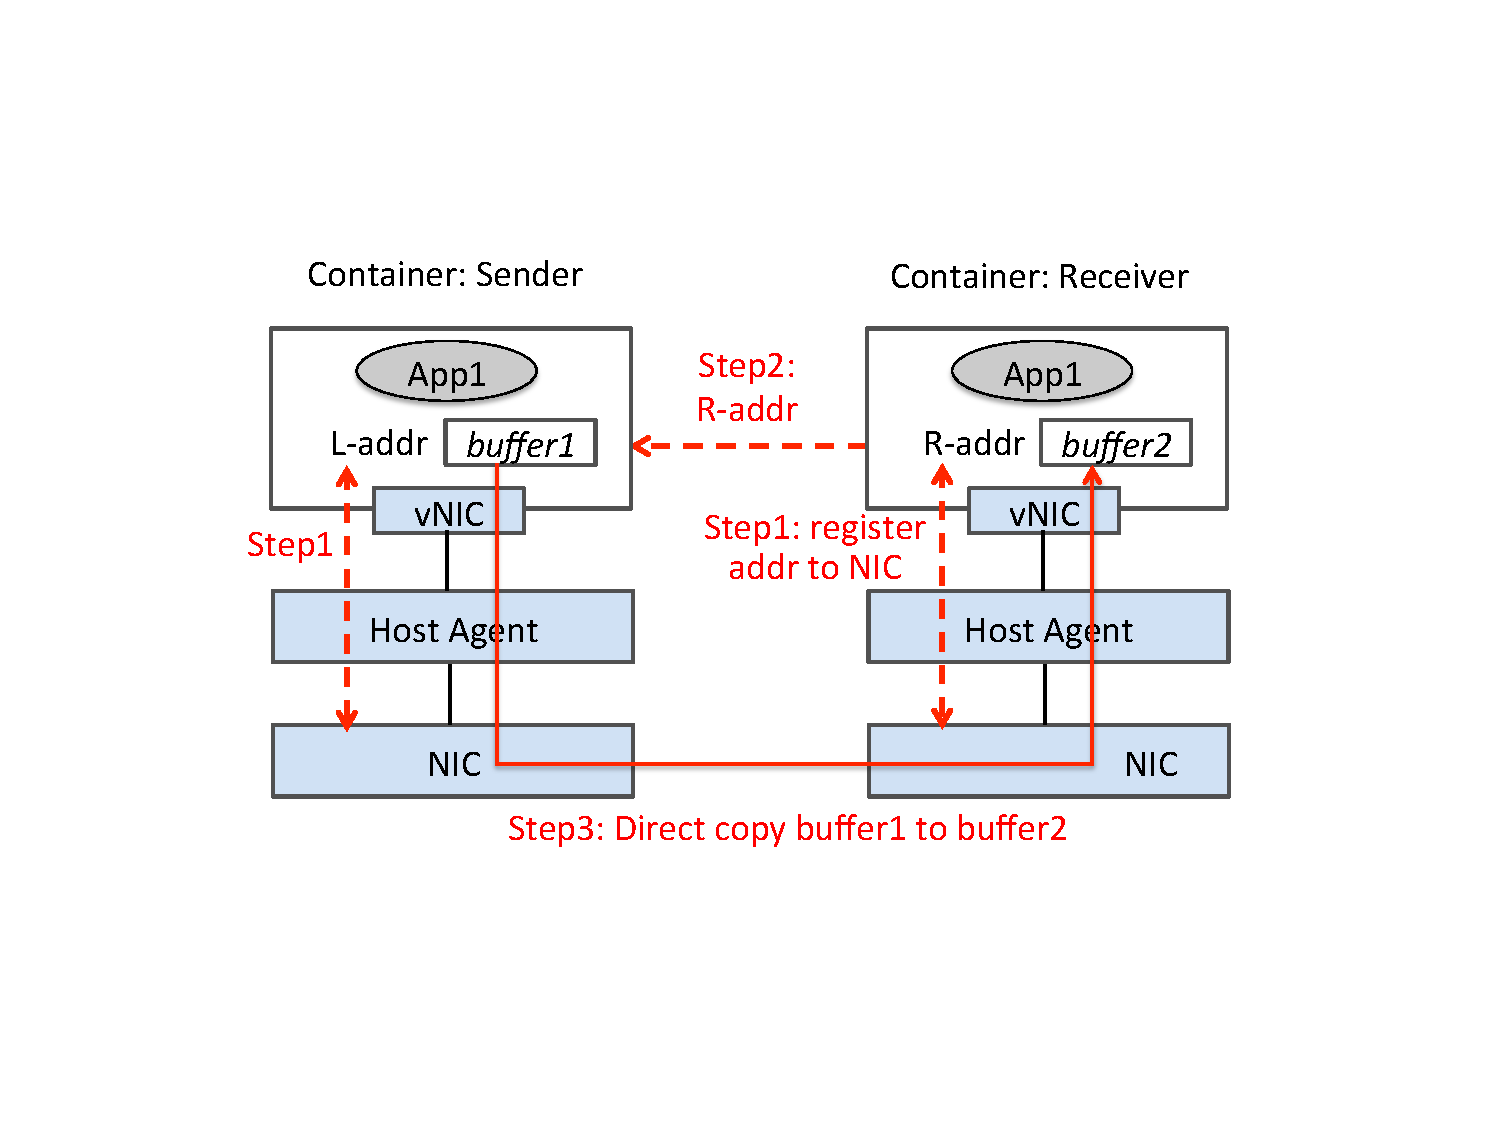
\includegraphics[width=0.45\textwidth]{figures/system/sys_rdma_rdma.pdf}      
     \label{fig:sys_rdma_rdma}
     \caption{How \sysname implemented RDMA write in inter-host setting.} 
     \end{figure}

In \sysname, both the sender and receiver containers have a virtual RDMA NIC.
In Step 1, the sender creates a shared-memory block and write data, and then 
the local network agent will get the pointer of this shared-memory block after the sender passes it to its virtual NIC; In Step 2, after receiving the IP of 
the receiver, the local network agent will check whether the receiver is on
the same host of the sender. If the answer is "Yes", the local network agent will
directly leverage the receiver's virtual NIC to notify it that a memory block 
from RDMA is ready to read with the pointer of the shared-memory block. 
Otherwise, the sender's local network agent will perform an actual RDMA write
with the receiver's local network agent, and the latter will put the received data into a shared-memory and pass it to the receiver container via its virtual NIC.
     
     \begin{figure}[ht]
     \centering 
     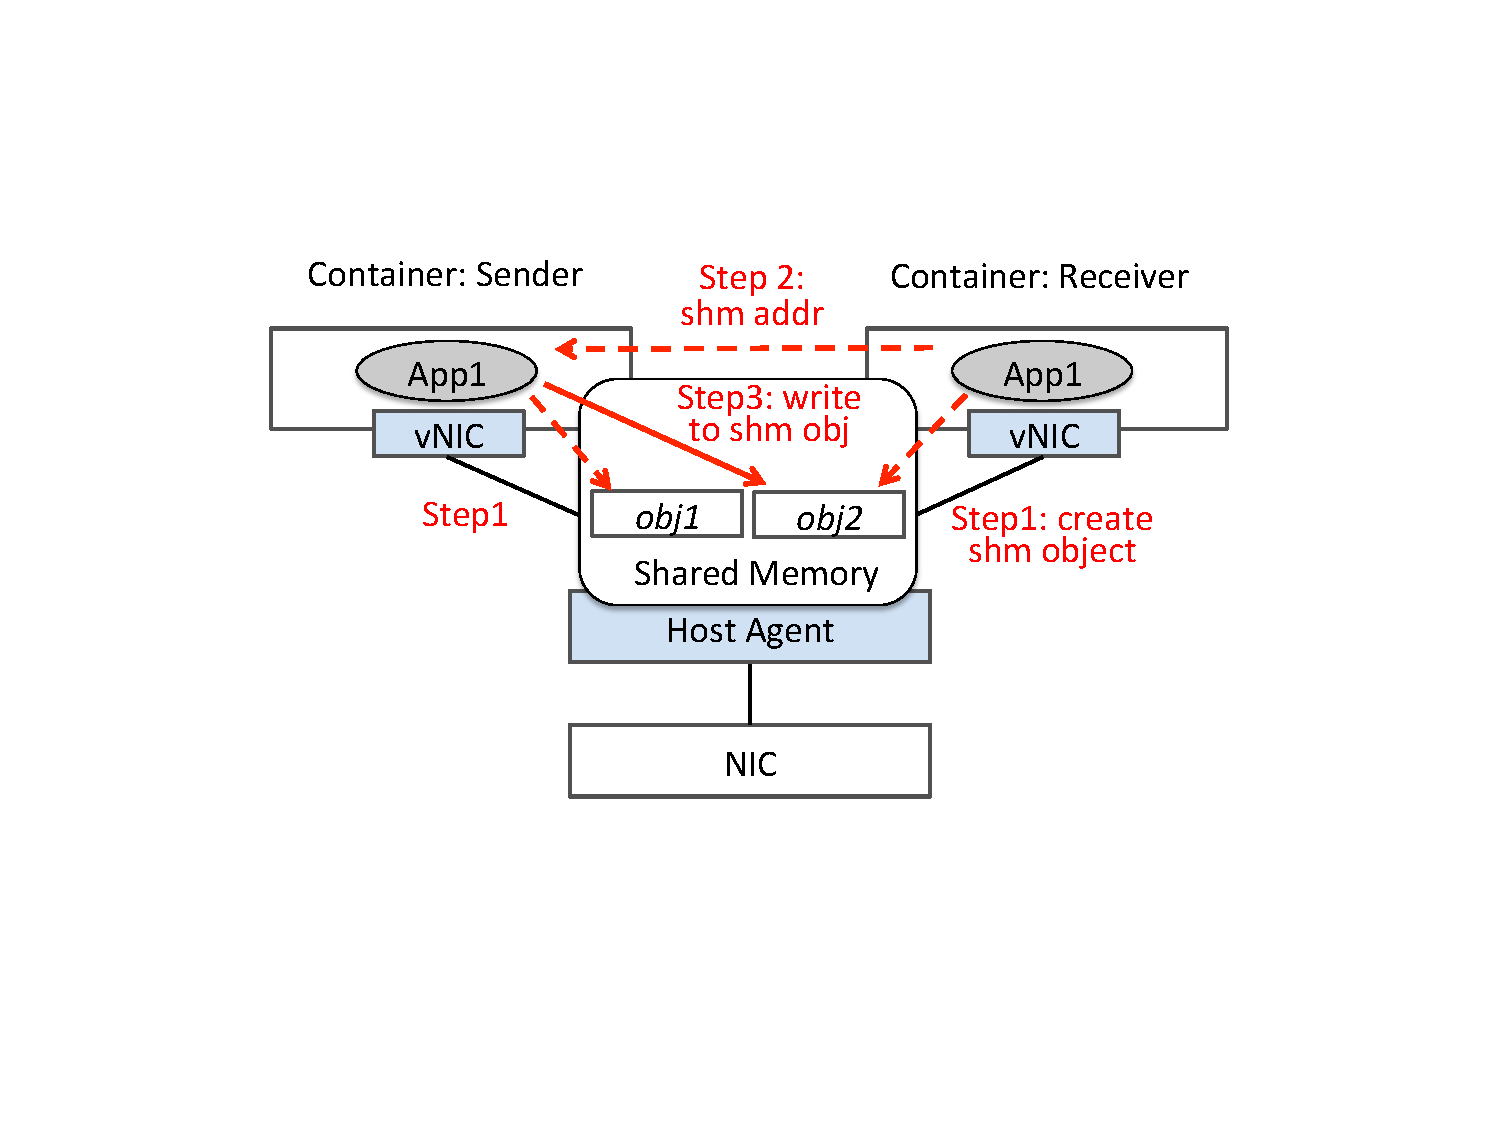
\includegraphics[width=0.45\textwidth]{figures/system/sys_rdma_shm.pdf}      
     \label{fig:sys_rdma_shm}
     \caption{How \sysname implemented RDMA write with shared memory in intra-host setting.} 
     \end{figure}
     


\iffalse

     \begin{figure}[ht]
     \centering 
     \begin{subfigure}
     \centering 
     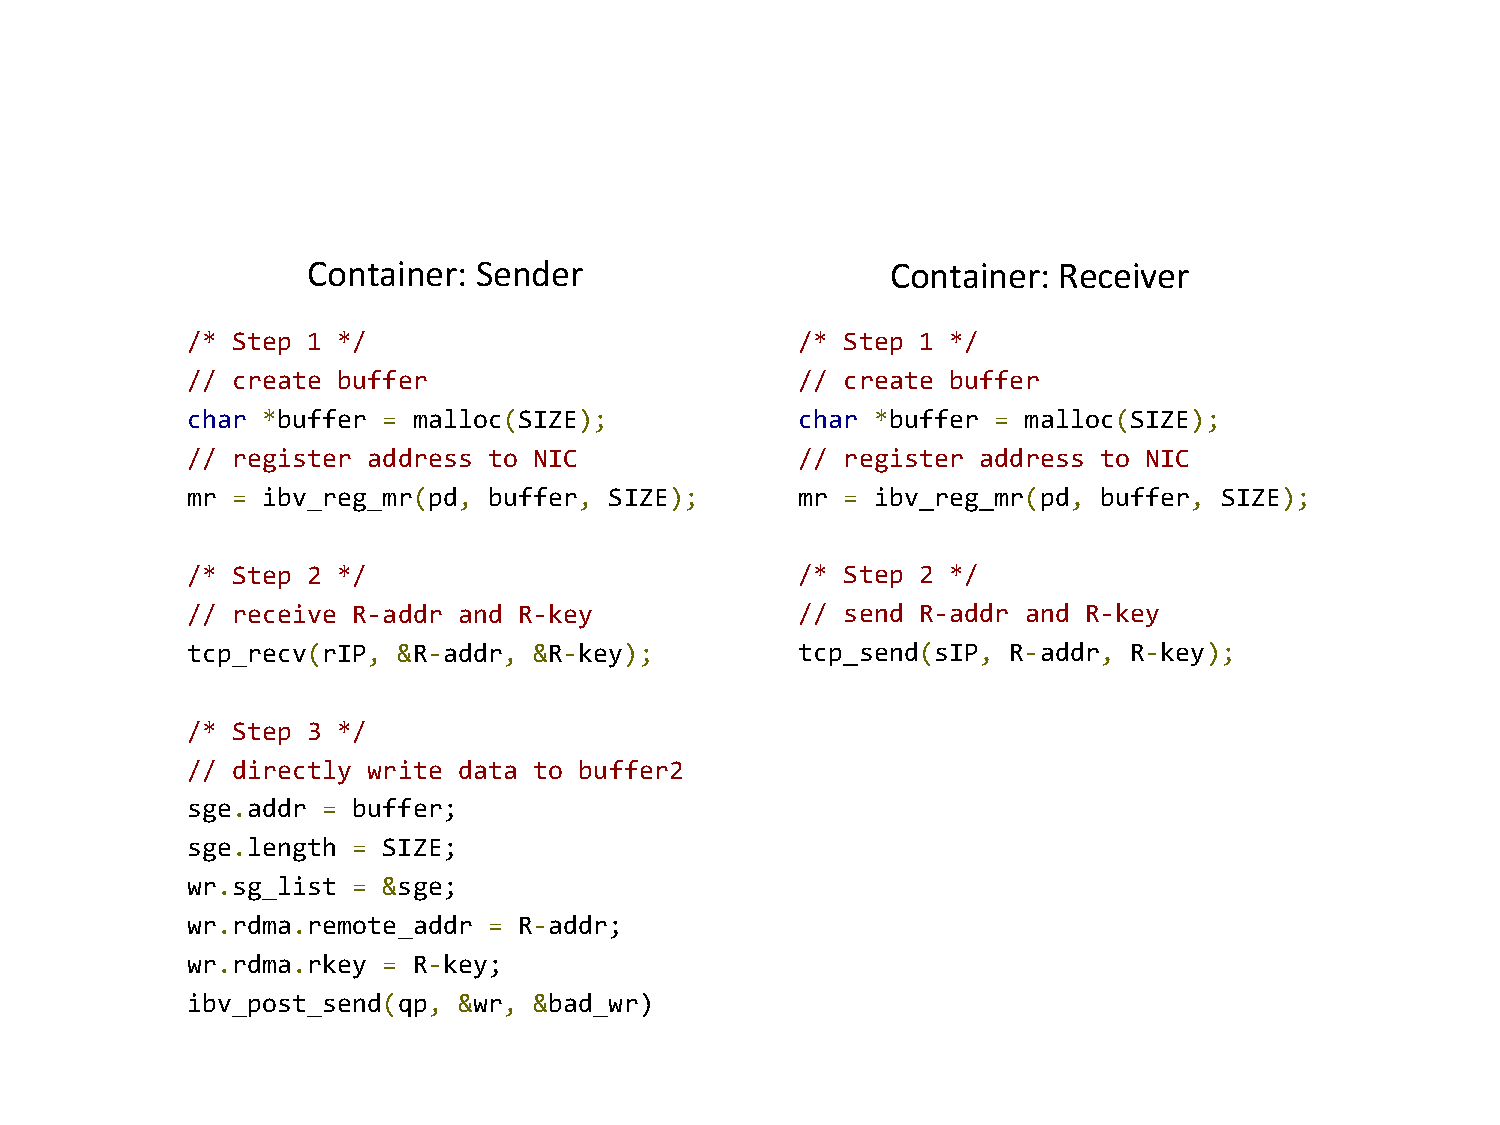
\includegraphics[width=0.45\textwidth]{figures/system/sys_rdma_code.pdf}
     %\caption{} 
     \end{subfigure}
           
     \begin{subfigure}
     \centering 
     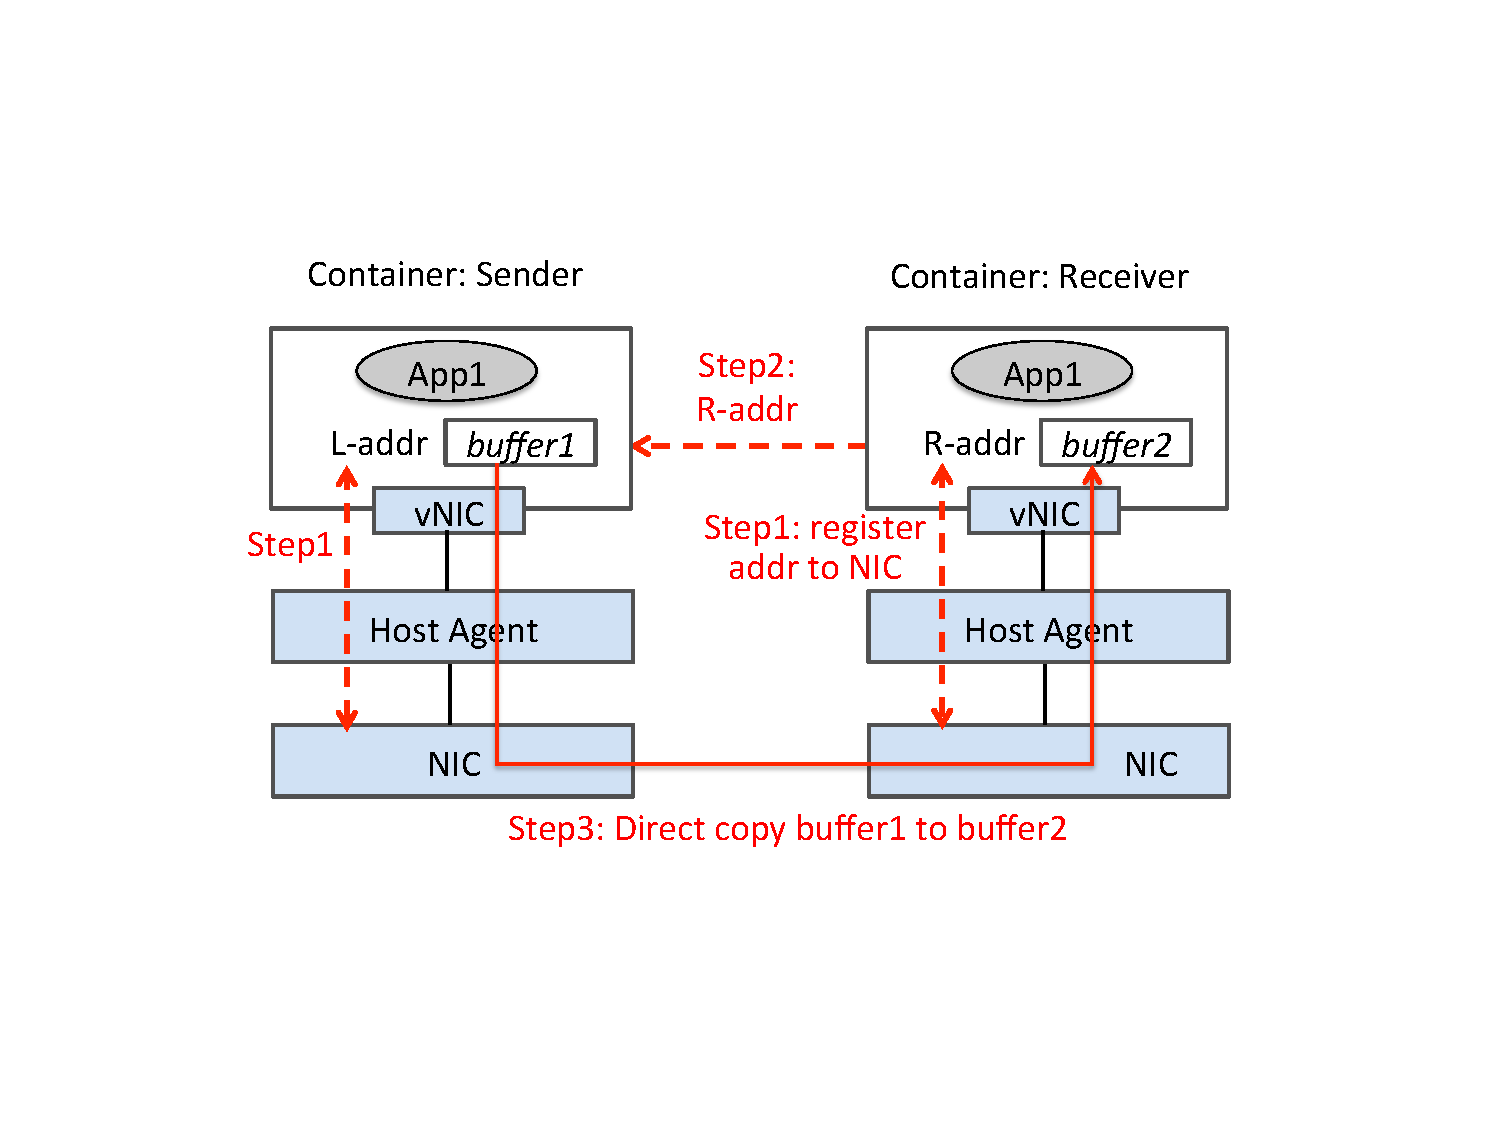
\includegraphics[width=0.45\textwidth]{figures/system/sys_rdma_rdma.pdf}      
     %\caption{} 
     \end{subfigure}
     
     \begin{subfigure}
     \centering
     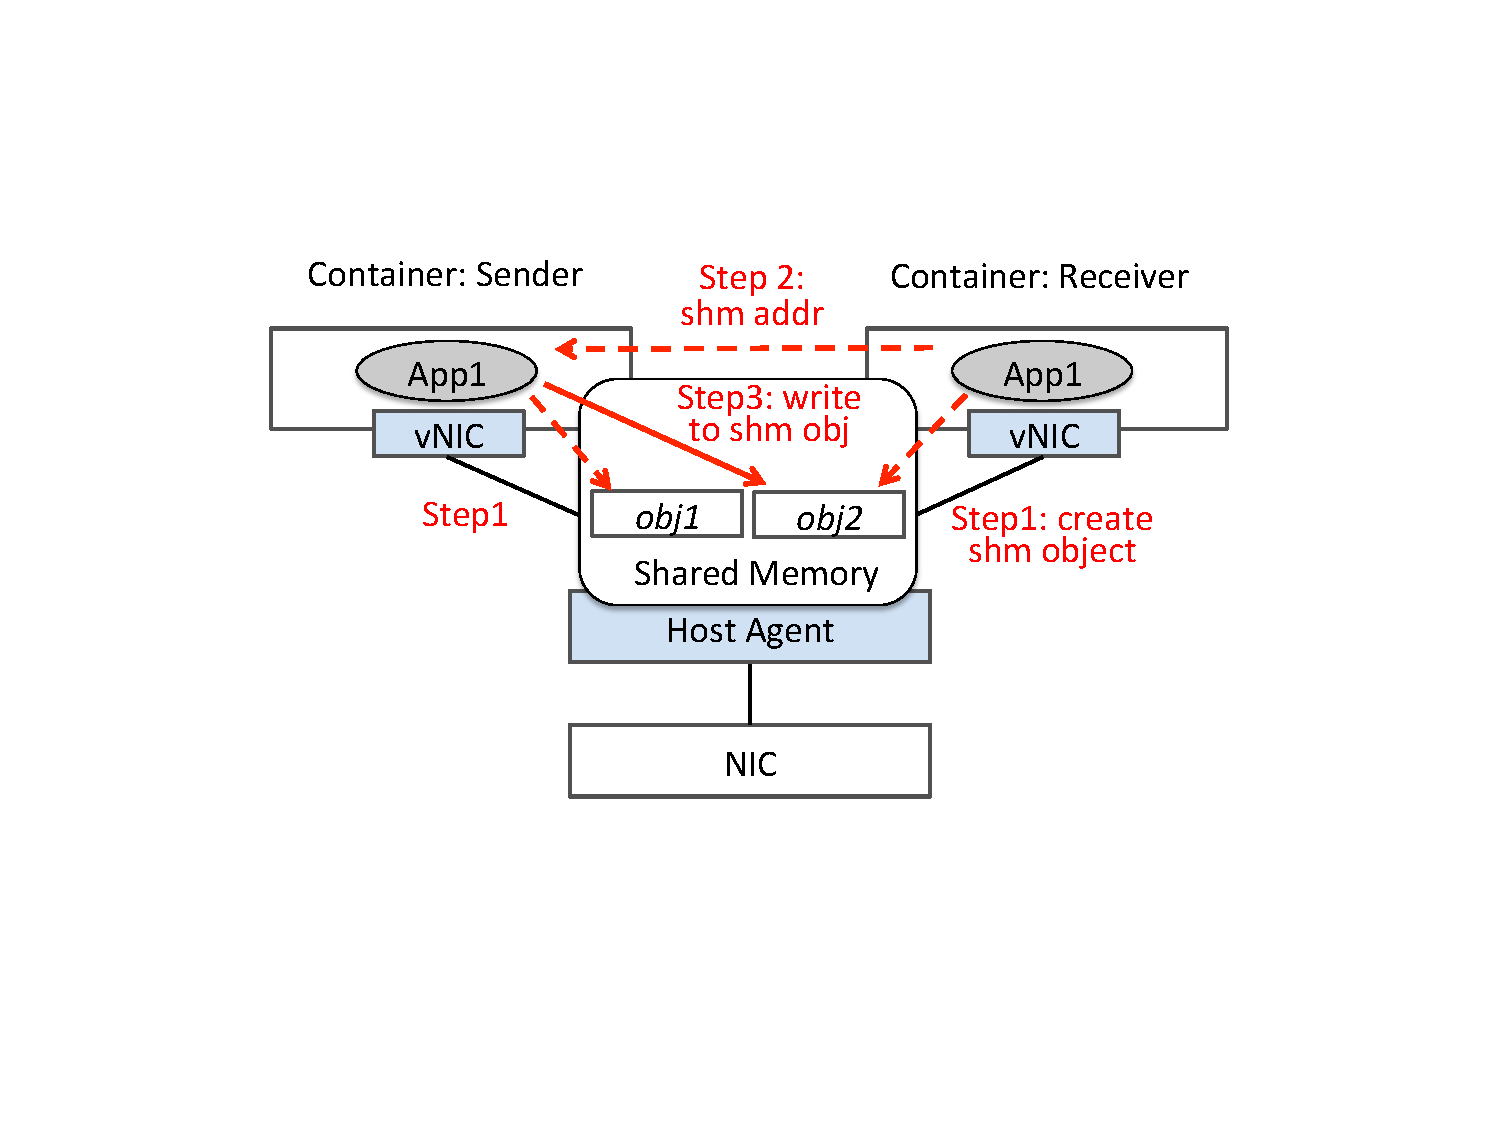
\includegraphics[width=0.45\textwidth]{figures/system/sys_rdma_shm.pdf}      
     %\caption{} 
     \end{subfigure}
     \label{fig:system_modules}
     \caption{The modules of \sysname.} 
     \end{figure}

%P1 introduce the two components we want to build
\sysname's main components includes a Orchestrator and a virtualized NIC.
The Orchestrator can figure out the most efficient way for two containers to talk with each other (e.g. 
via shared memory, rdma or dpdk) based on the location of the container or the resource
utilization of the host.
And the virtualized NIC emulates the necessary underlying resource structures 
(e.g., send queue or receive queue for RDMA). In this way, the application can
gain the desired \emph{portability}, since the application can now use the standardized  
APIs without being aware of the various underlying communication
mechanisms in different environments. 
Both of the components are shown in Figure~\ref{fig:system_modules}.

     \begin{figure}[ht]
     \centering 
     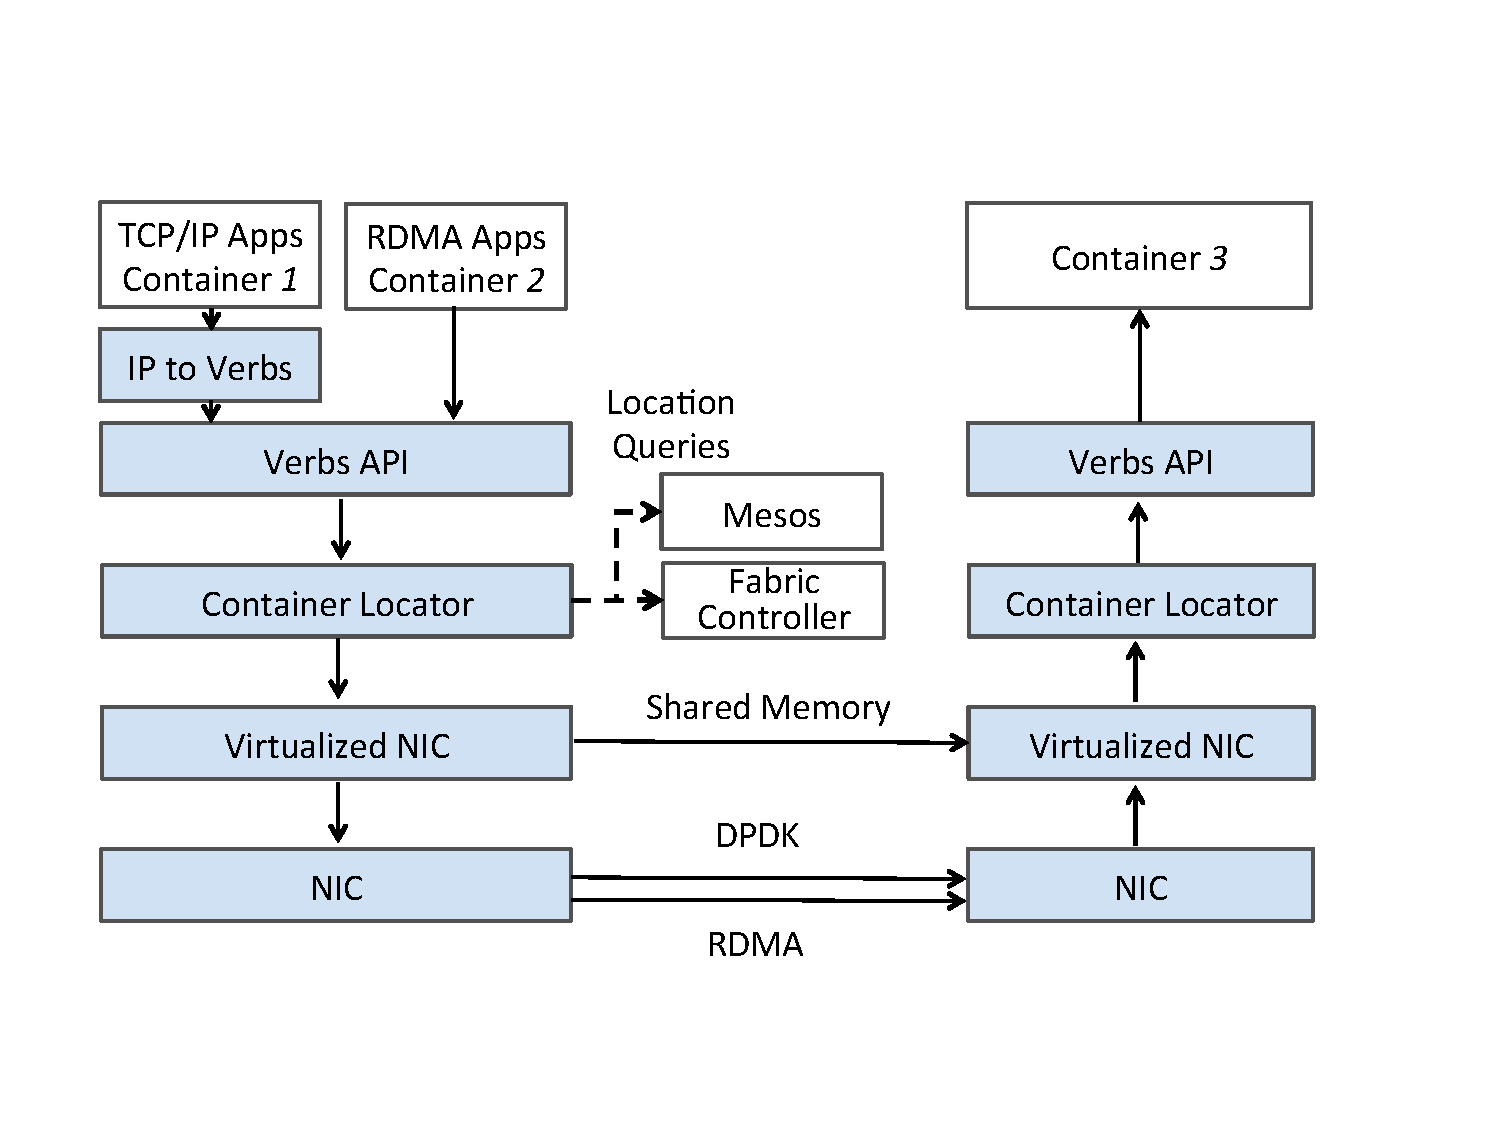
\includegraphics[width=0.45\textwidth]{figures/system/system_modules.pdf}      
     \label{fig:system_modules}
     \caption{The modules of \sysname.} 
     \end{figure}
     
      \begin{figure}[ht]
         \centering 
         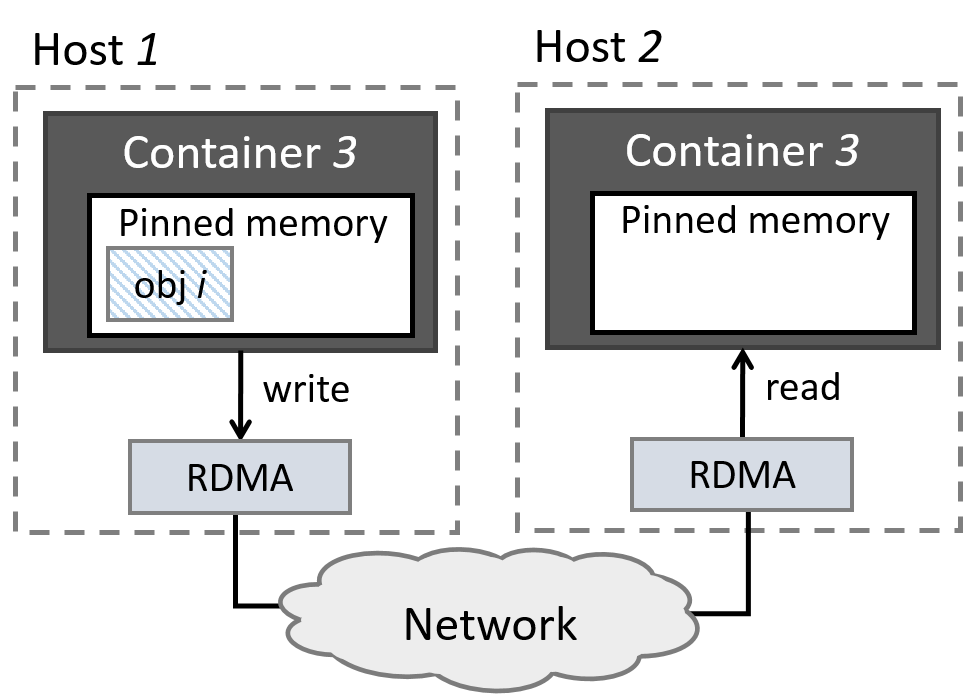
\includegraphics[width=0.2\textwidth]{figures/rdma-container.png}   
         \caption{??}   
      \end{figure}
      
      \begin{figure}[ht]
      	\centering 
      	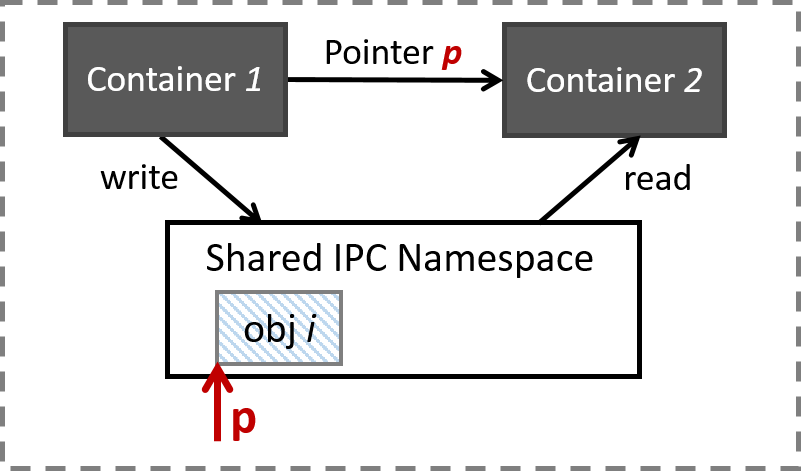
\includegraphics[width=0.2\textwidth]{figures/shared-mem-container.png}   
      	\caption{??}   
      \end{figure}

\subsection{Virtualized NIC}
The virtualized NIC (vNIC) a transparent layer between the application and the underlying network structure.
We modify the communication libraries of a container so the vNIC can intercept on the communication requests
from the applications (e.g. send request). For example, if the application is a RDMA application, we
will modify the library \texttt{libibverbs} to pass verbs calls to the vNIC.

The virtualized NIC has two roles. First, it queries the Orchestrator for the best mechanism to implement the 
communication requests, as illustrated in Figure~\ref{fig:system_modules}.
For example, if the two containers are intra-VM, it will create a shared namespace and memory objects 
for the two containers, and write the sender's data into the shared memory objects and pass the pointers of the
memory objects to the receiver container to transfer the data.

Second, the virtualized NIC (vNIC) emulates underlying network structure. 
For example, for RDMA, the vNIC will emulate the data structures including the Send Queue, 
Receive Queue, Completion Queue and Queue Pairs.
In this way, the vNIC not only maintains compatibility with currently written applications, but also
gain the desired \emph{portability}. Because the containers applications no longer need to bind to
the underlying network structure (bind to the vNIC instead), and the vNIC can be ported along with
the applications.

% as a emulation  underlying network structure
%a transparent layer between the application and the underlying network structure, dynamically choosing the best communication mechanism, while maintaining compatibility with currently written applications.

%The decision of which mechanism to chose is based on the hardware capabilities of the hosts and the physical placement of the containers, while aiming for minimal CPU overhead and high throughput. This decision and switching between communication mechanism is done completely transparent from application.

%For intra-host communication, virtualized NIC will use shared memory communication inducing minimal pressure on the CPU while reaching high throughput (~ memory bandwidth). For inter-host communication, the virtualized NIC will prioritize RDMA communication when supported by the underlying hardware. Otherwise, it will use TCP/IP communication. 


\subsection{Orchestrator}
The Orchestrator is a logic module to intelligently decide the most
efficient way to implement the communication request based on the locations
of the containers or the resources utilization of the host.

     \begin{figure}[ht]
     \centering 
     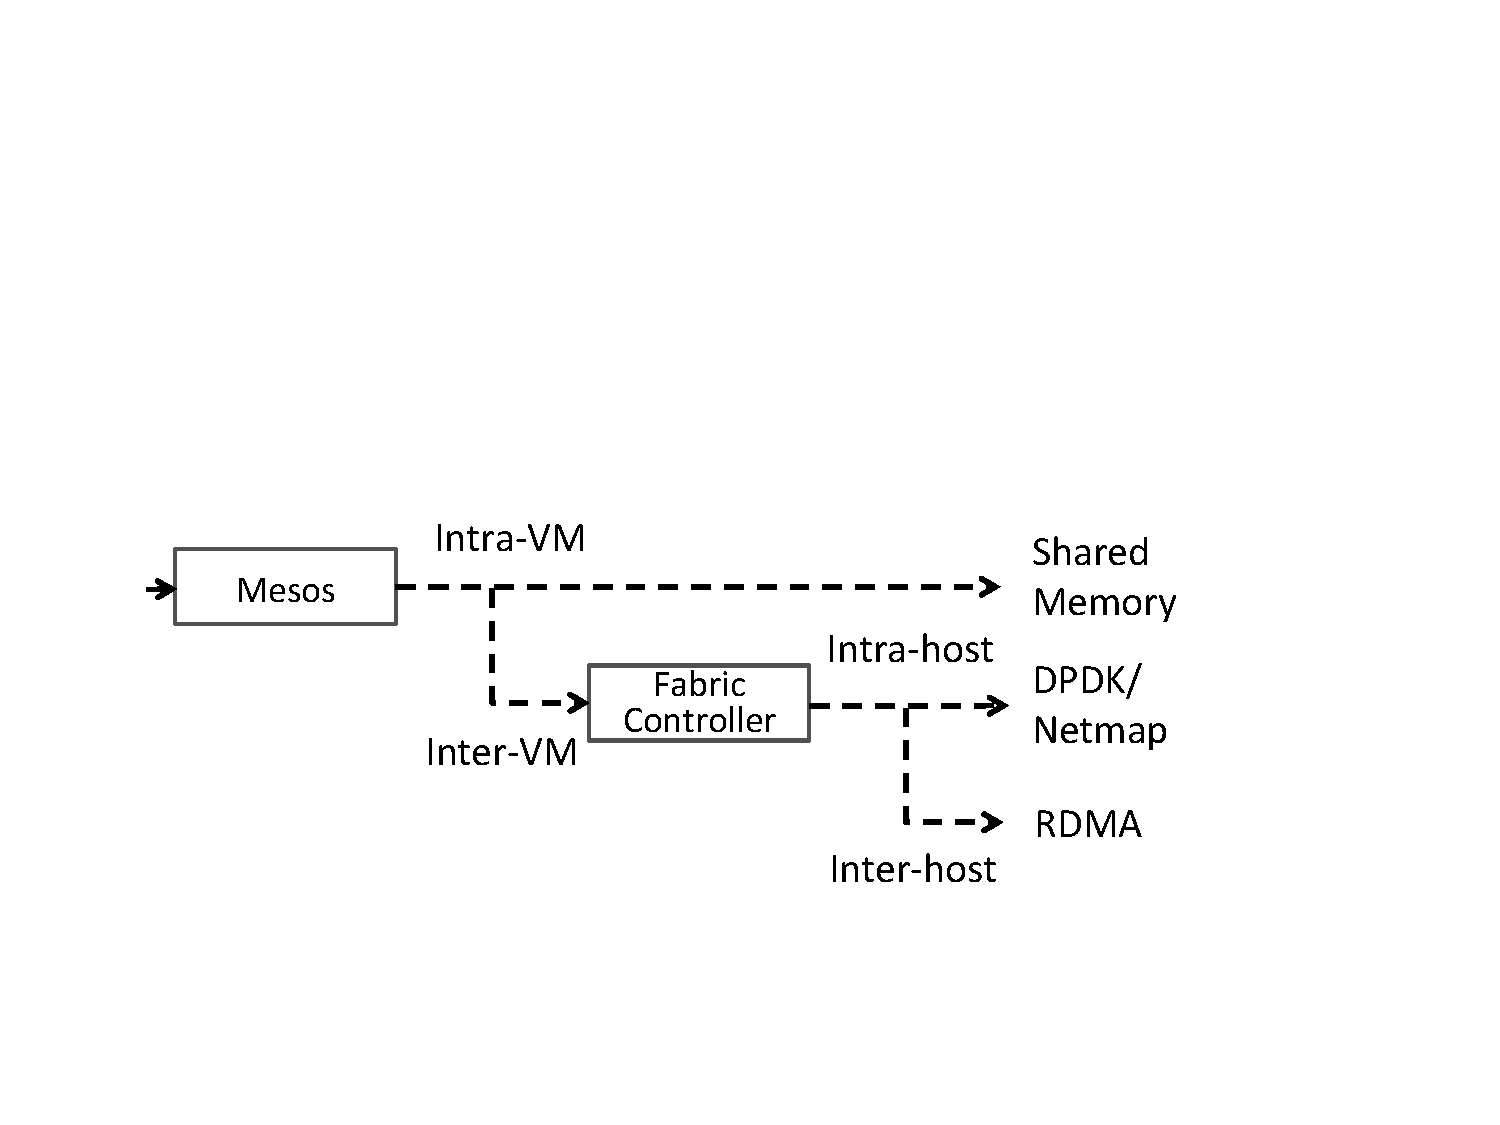
\includegraphics[width=0.45\textwidth]{figures/system/system_locator.pdf}      
     \label{fig:system_locator}
     \caption{The logic flow of Orchestrator.} 
     \end{figure}

Suppose the decision is only based on the location of the containers, the logic will be as follows.
The Orchestrator send queries to Mesos (resource manager) and the cloud's Fabric Controller to locate
the sender/receiver containers and decide the most efficient way they talk with each other.
The logic flow of this process is as shown in Figure~\ref{fig:system_locator}.
For example, given a send request, the Orchestrator will query Mesos to figure out if the 
sender/receiver containers are intra-VM or inter-VM. 
For intra-VM containers, the Orchestrator will raise a flag to notify the virtualized NIC to
send the data via shared memory.
For inter-VM containers, the Orchestrator will then quire if the two containers are intra-host
or inter-host.
If the containers are inter-VM but intra-host, Orchestrator will tell the virtualized NIC to send
the data via fast data pass across VMs in the same machine, such as NetVM\cite{} or netmaps\cite{}.
Or if the containers are inter-host, RDMA would be the most efficient way to perform the data transfer.

\tianlong{There should be some design decisions to support the above logic in design section.}

%We are going to add a logic module called Orchestrator inside the application's
%library for communication. For example, the  

\subsection{Put It Together}
Now let's put the components together and see the workflow of \sysname, as shown in Figure~\ref{fig:system_modules}.
Let's take two rdma applications (in container2 and container3) as an example.
Suppose application in container2 (app2 in short) issues a send data to container3 request via standardized Verbs API.
The vNIC will intercept the request and query the Orchestrator. 
Then the orchestrator will query Mesos or Fabric Controller to obtain the locations of 
container2 and container3. Then Orchestrator will send a decision of the best mechanism to the vNIC.
The request will call to the emulated data structures in the vNIC (e.g. QP, SQ, RQ, CQ). And the vNIC will choose the
best mechanism (e.g. RDMA, shared memory, dpdk/netmap) to implement the request. For example, if the containers
are inter-host, RDMA will be selected. If the best mechanism is not available (e.g. NIC lack of RDMA support), it will
fall back to the sub-optimal mechanism (e.g., TCP/IP).

\fi
\section{Discussions} \label{sec:discussion}

\textbf{Live migration:} 
\sysname could be a key enabler
for containers to achieve both high-performance and capability for live
migration. It will require the network library to interact with the orchestrator
more frequently, and may require maintaining additional per-connection state
within the library. We are currently investigating this further.

\textbf{Security and middle-box:} One valid concern for \sysname is how legacy
middle-boxes will work for communication via shared-memory or RDMA, and whether
security will be broken by using shared-memory or RDMA.  We do not yet have
complete answer to this issue. We envision that for security, \sysname would
only allow shared-memory among trusted containers, for example, container
belongs to the same vendor (e.g., running spark or storm).  We are investigating
how best to support existing middle-boxes (e.g. IDS/IPS) under \sysname.


\textbf{VM environment:}
So far our evaluation and prototype is based on containers running on
bare-metal.  But our design easily generalizes to containers deployed inside
VMs. Some issues, such as efficient inter-VM communication (perhaps using
NetVM~\cite{netvm}) need to be addressed, but we believe that it can be easily
done within the context of \sysname design.

%\textbf{Network trouble shooting:}

%\textbf{VM environment:}
%So far our evaluation and prototype is based on containers running on bare-metal. 
%Although we believe our design is also general for containers deployed inside VMs,
%the VM environment can brought in further challenges such as how to handle the
%address mapping, how to enable shared-memory/RDMA or how to locate the containers
%and measure the utility of resources. We will address these challenges in our futureworks.

\section{Related Work} \label{sec:related}

%NetVM  \cite{netvm}
%DPDK and NetMap \cite{netmap}

\textbf{Inter-VM Communication:} 
The tussle between isolation and performance is not unique to containers.
In the field of Inter-VM Communication, there are several works that provides
high-performance by removing some of the isolation constraints.
For example, NetVM\cite{netvm} provides a shared-memory framework that
exploits the DPDK library to provide zero-copy delivery between VMs.
Netmap\cite{netmap} and VALE\cite{vale} (which is also used by ClickOS\cite{clickos}) 
are sharing buffers and metadata between kernel and userspace to eliminate memory copies.
However, these works actually strengthened the binding between VM and underlying host
structures, thus they cannot satisfy the portability requirement for \sysname. 
Also, the NetVM work is applicable only to intra-host setting,
constrained by the possibility of shared memory. Similarly, the Netmap
and VALE solutions are sub-optimal when the VMs/containers are located
on the same physical machine.

\textbf{RDMA and HPC:} RDMA originated from the HPC world, in the form of InfiniBand. The HPC
community proposed RDMA enablement solutions for
virtualization~\cite{ranadive2012toward} and
containerization~\cite{rdmacontainers} technologies. These solutions
are addressing the challenges in exposing RDMA interfaces to
virtualized/containerized applications, treating each VM/container as
if it resides on a different node.

The HPC community have also been using shared-memory based
communication~\cite{KNEM,MPI:p:MPI,HybridMPI} for intra-node
communication. These solutions are targeting MPI processes residing on
a shared non-containerized, non-virtualized machine. They do not
attempt to pierce the virtualization/containerization for additional
performance.

The same concepts described for \sysname can also be applicable for
MPI run-time libraries. This can be achieved either by layering the
MPI implementation on top of \sysname, or by implementing a similar
solution in the MPI run-time library.

\textbf{General improvements}
%low latency socket

%http://facweb.cti.depaul.edu/jyu/Publications/Yu-Linux-TSM2004.pdf
%High performance networking using SR-IOV \cite{highsriov}


%\cleardoublepage
%\bibliographystyle{abbrv}
%\bibliography{all_hotnets}

\end{document}
